\newpage
\begin{figure*}[!t]
\begin{narrow}{-1.2cm}{-1.2cm}\centering\vspace{-1.0cm}
\textbf{1. LCA with trigonometric and Kaiser windows - Capon shining}\\
\begin{tabular}[c]{l l l l}
\bf General & M = 32                            & $\Delta r = \frac{c}{2B}$ = 2.5 cm & $\frac{640\,\text{pixels}] / 12\,\text{m}}{\Delta r} = \frac{4}{3}$ \\
\bf LCA     & $\beta \in [0,10]$ (9 values) & $\phi \in [-1.07,1.07]$ deg (9 values) & Navg = 3 \\
\bf Capon   & $\Delta$ = 0.01                 & L = 16                           & Navg = 3 \\
\end{tabular}
\subfloat[LCA Window Response]{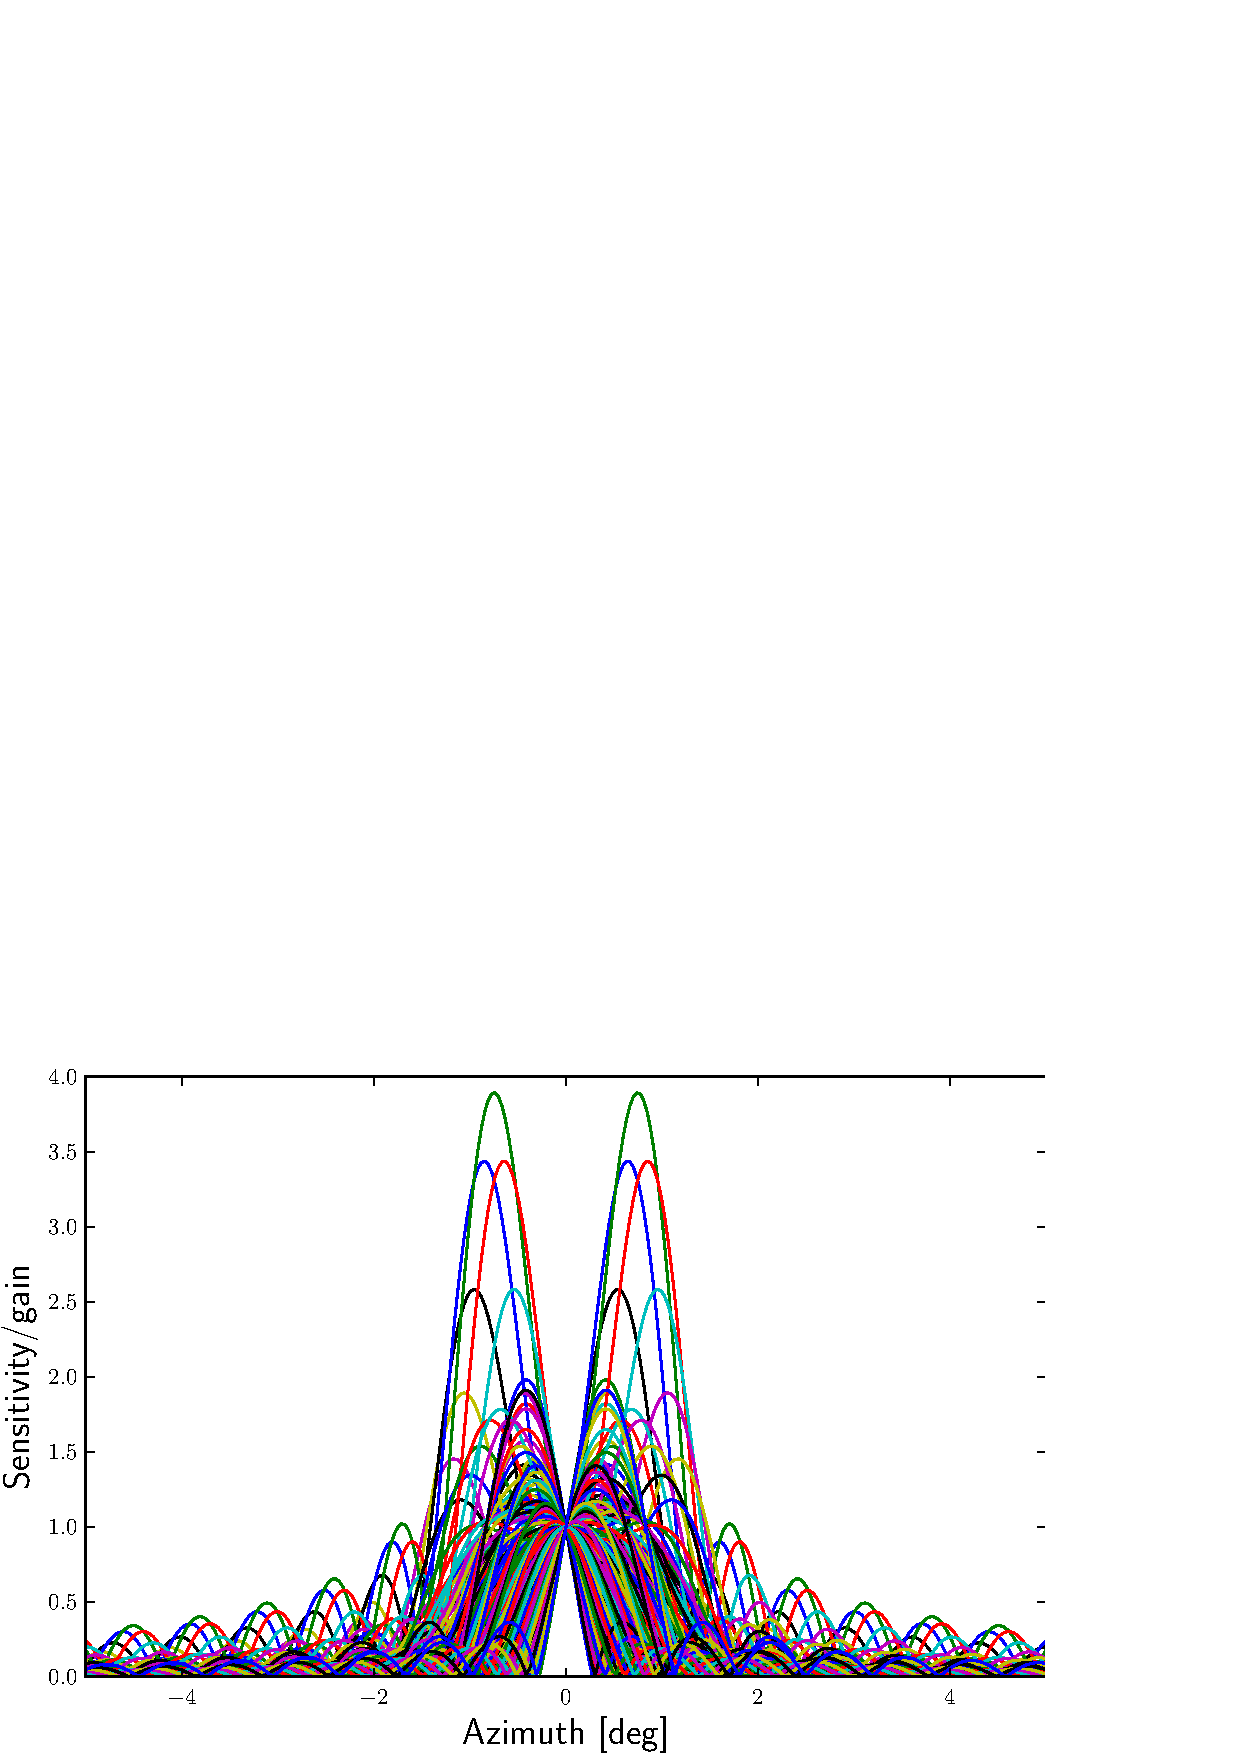
\includegraphics[width=0.49\linewidth]{gfx/1_window_response.png}}\hfill
\subfloat[Mean images]{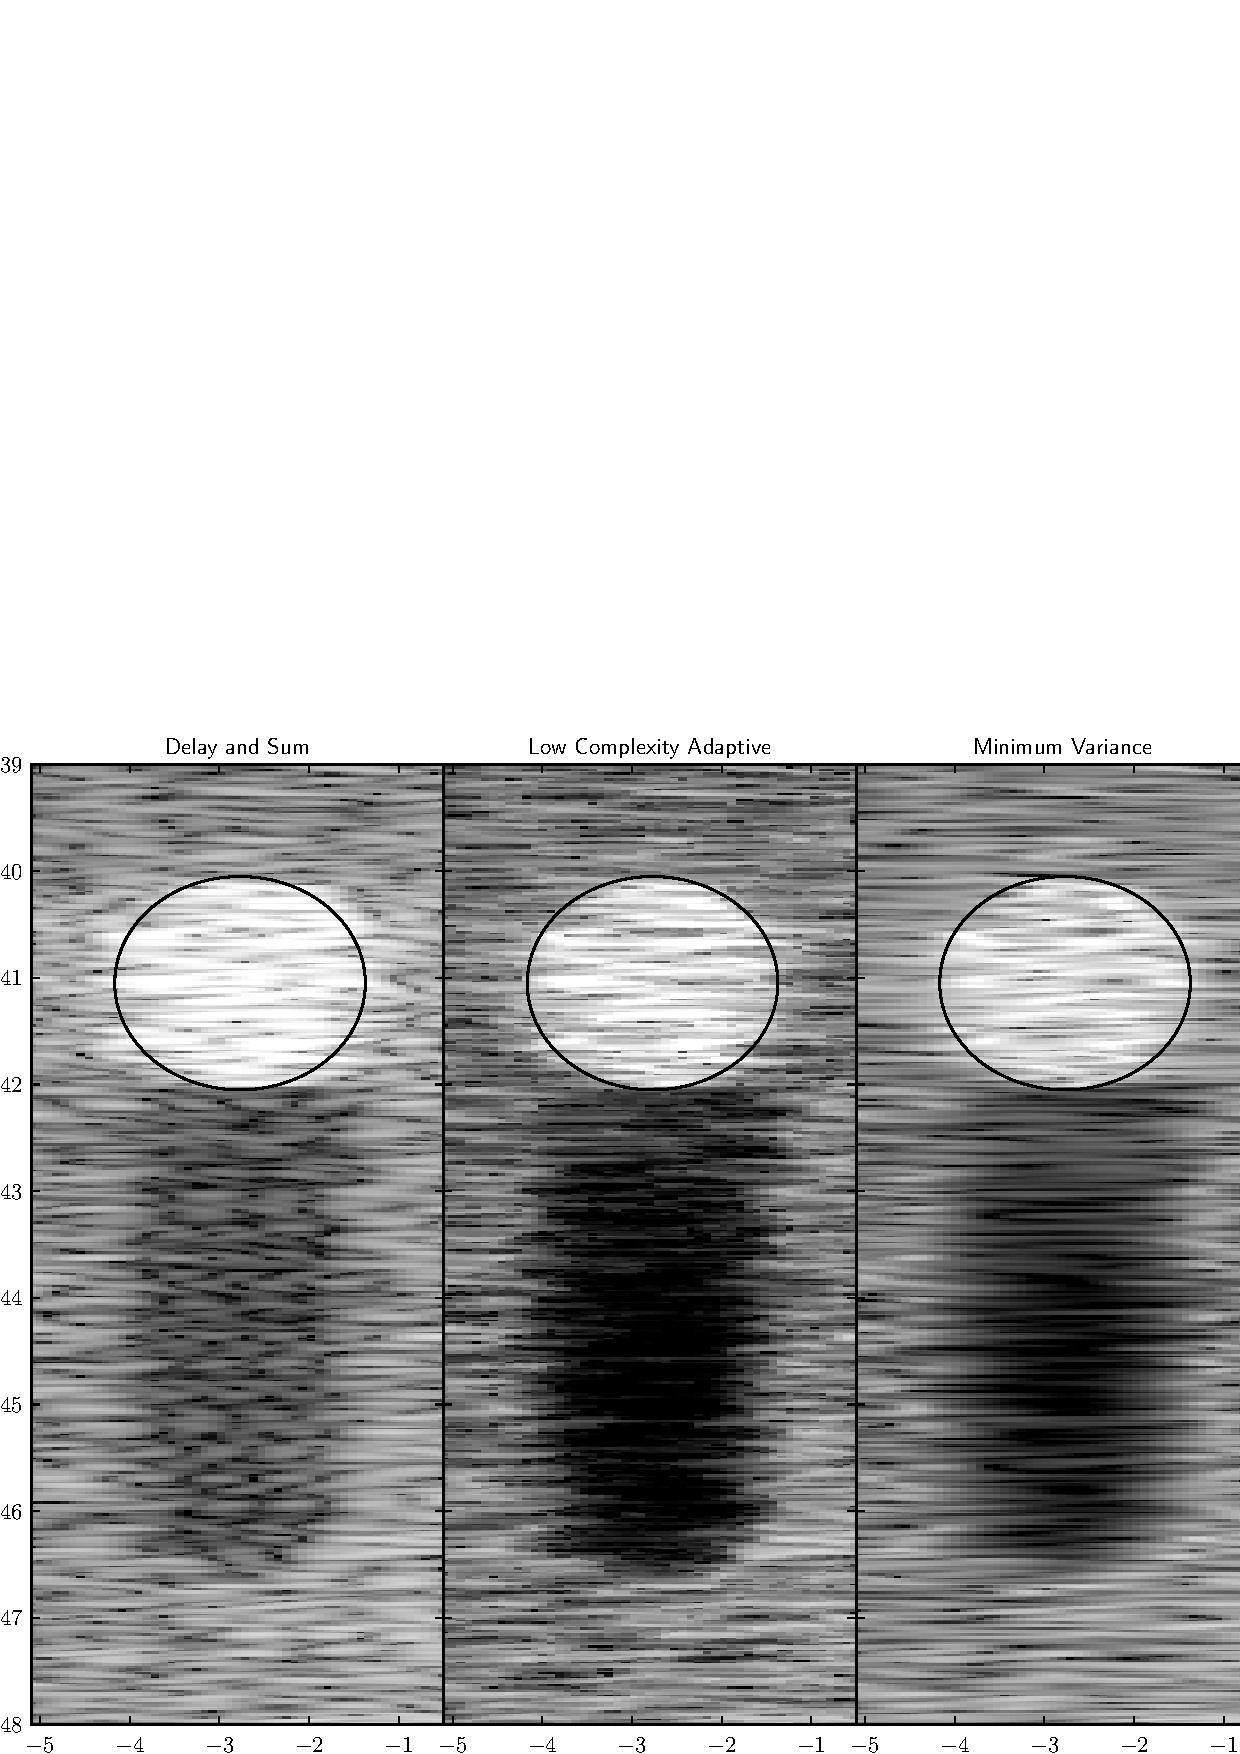
\includegraphics[width=0.49\linewidth]{gfx/1_mean_imgs.png}}\\
\subfloat[Windows ($\beta$)]{\includegraphics[width=0.49\linewidth]{gfx/1_windows_beta.png}}\hfill
\subfloat[Windows ($\phi$)]{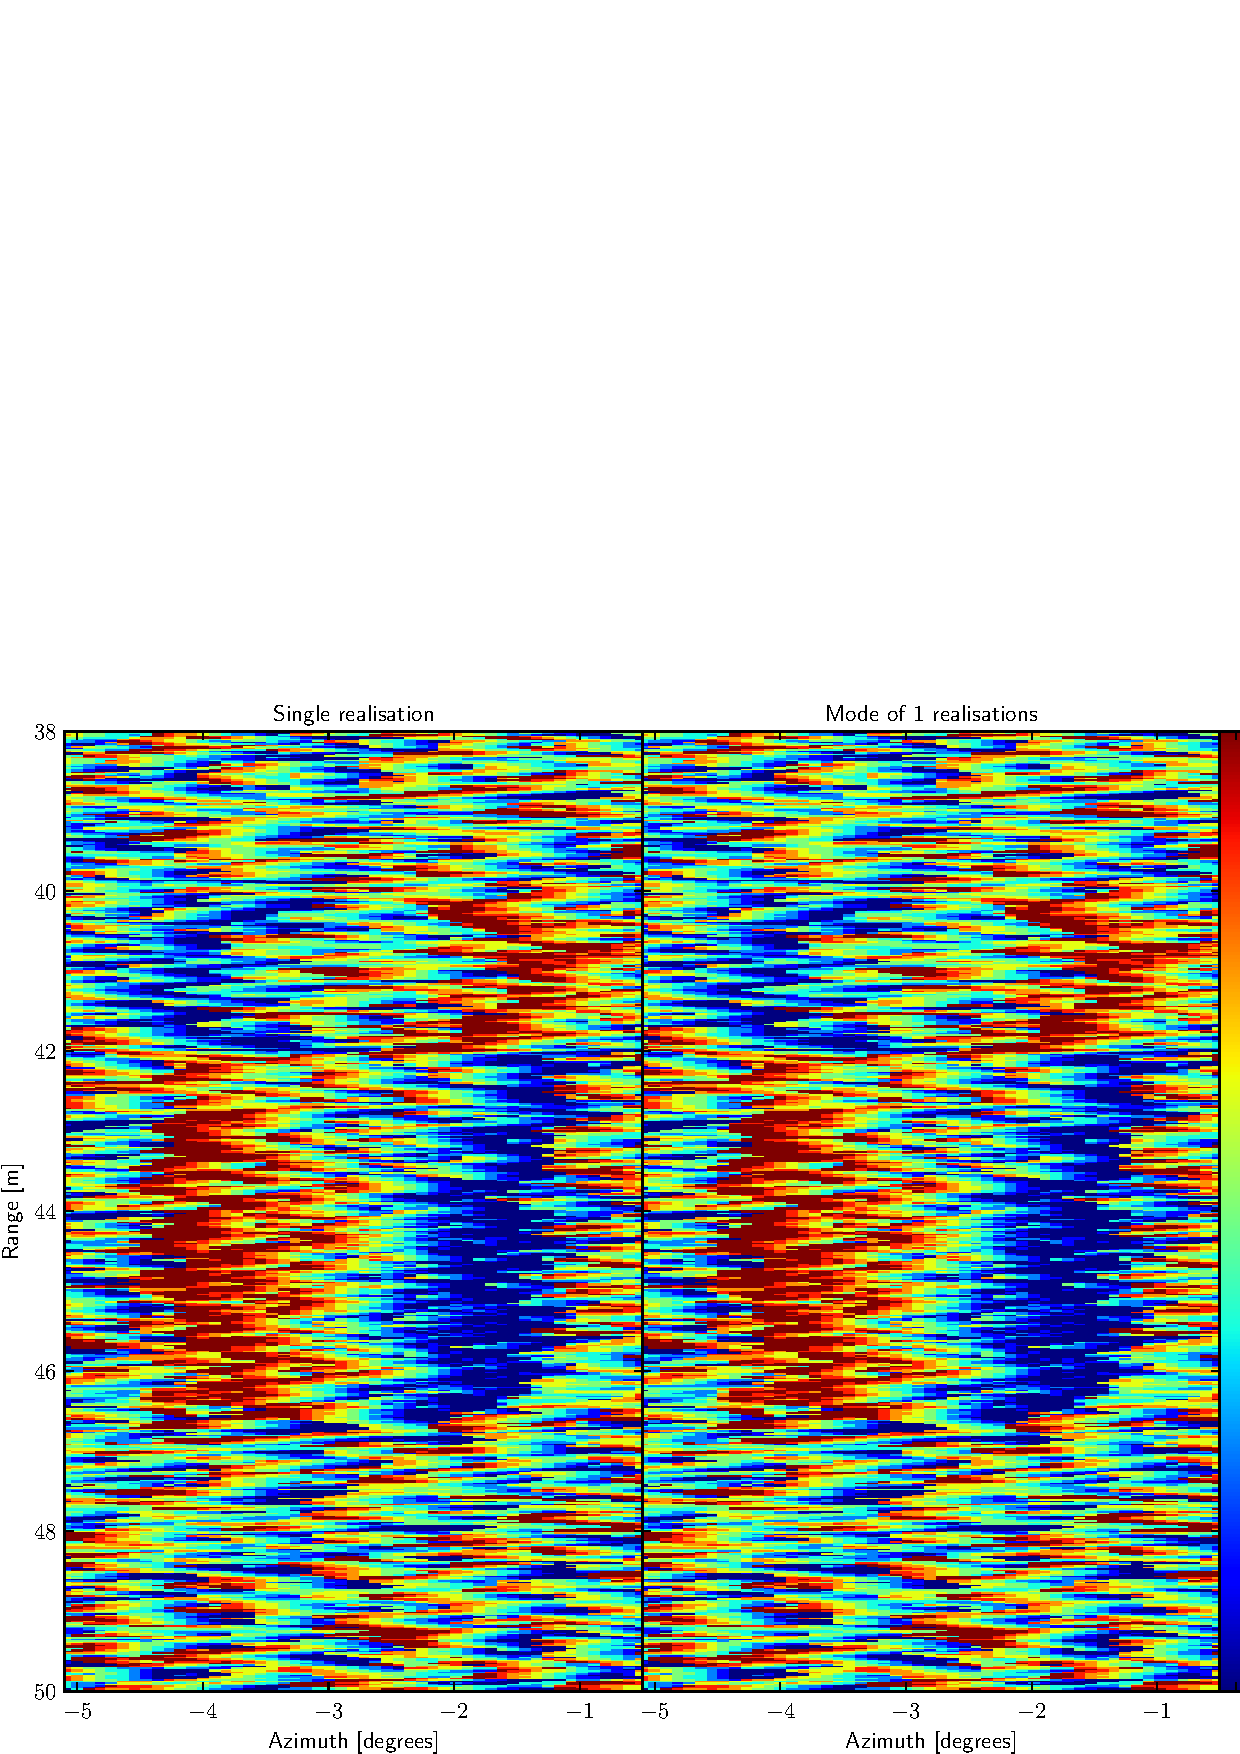
\includegraphics[width=0.48\linewidth]{gfx/1_windows_phi.png}}\\
\subfloat[Capon win. resp. through shadow]{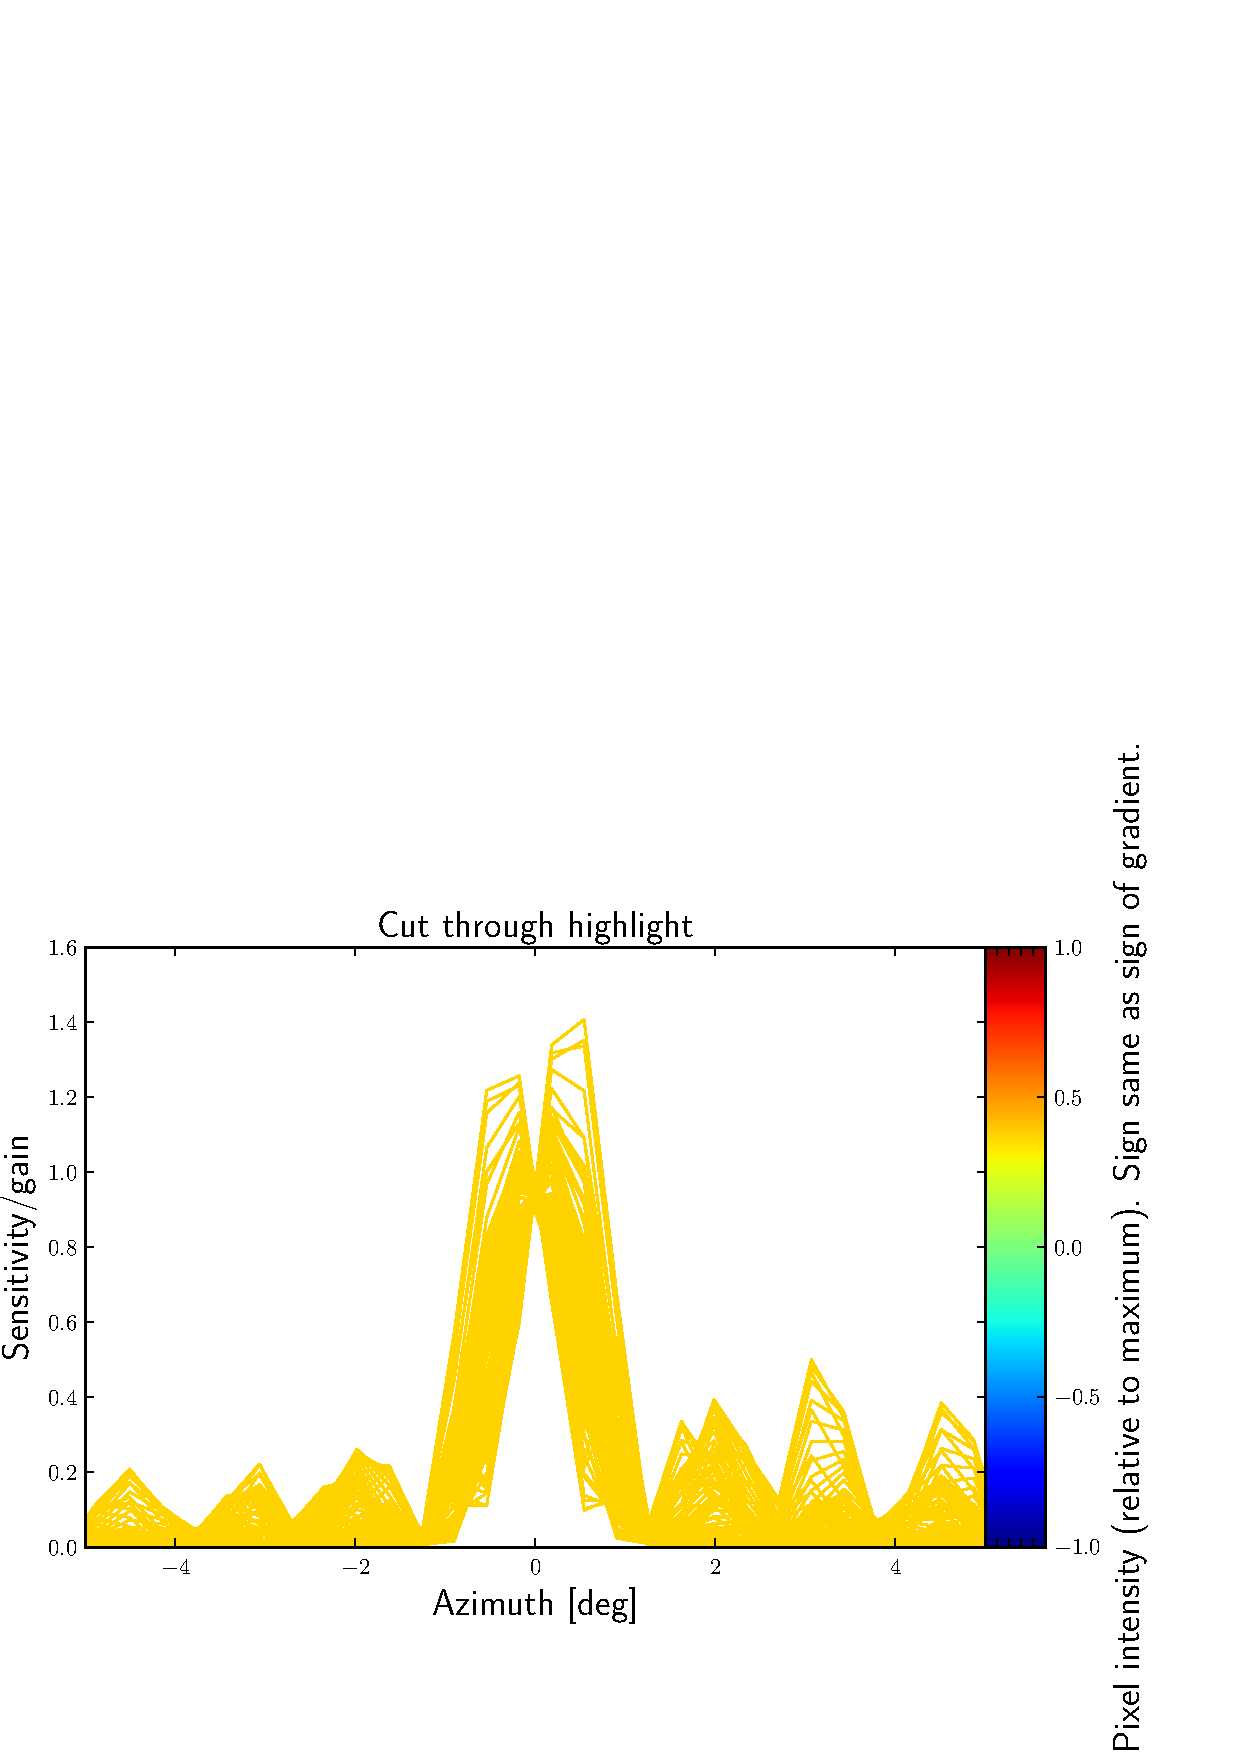
\includegraphics[width=0.49\linewidth]{gfx/1_win_resp_cut_shadow.png}}\hfill
\subfloat[Capon win. resp. through highlight]{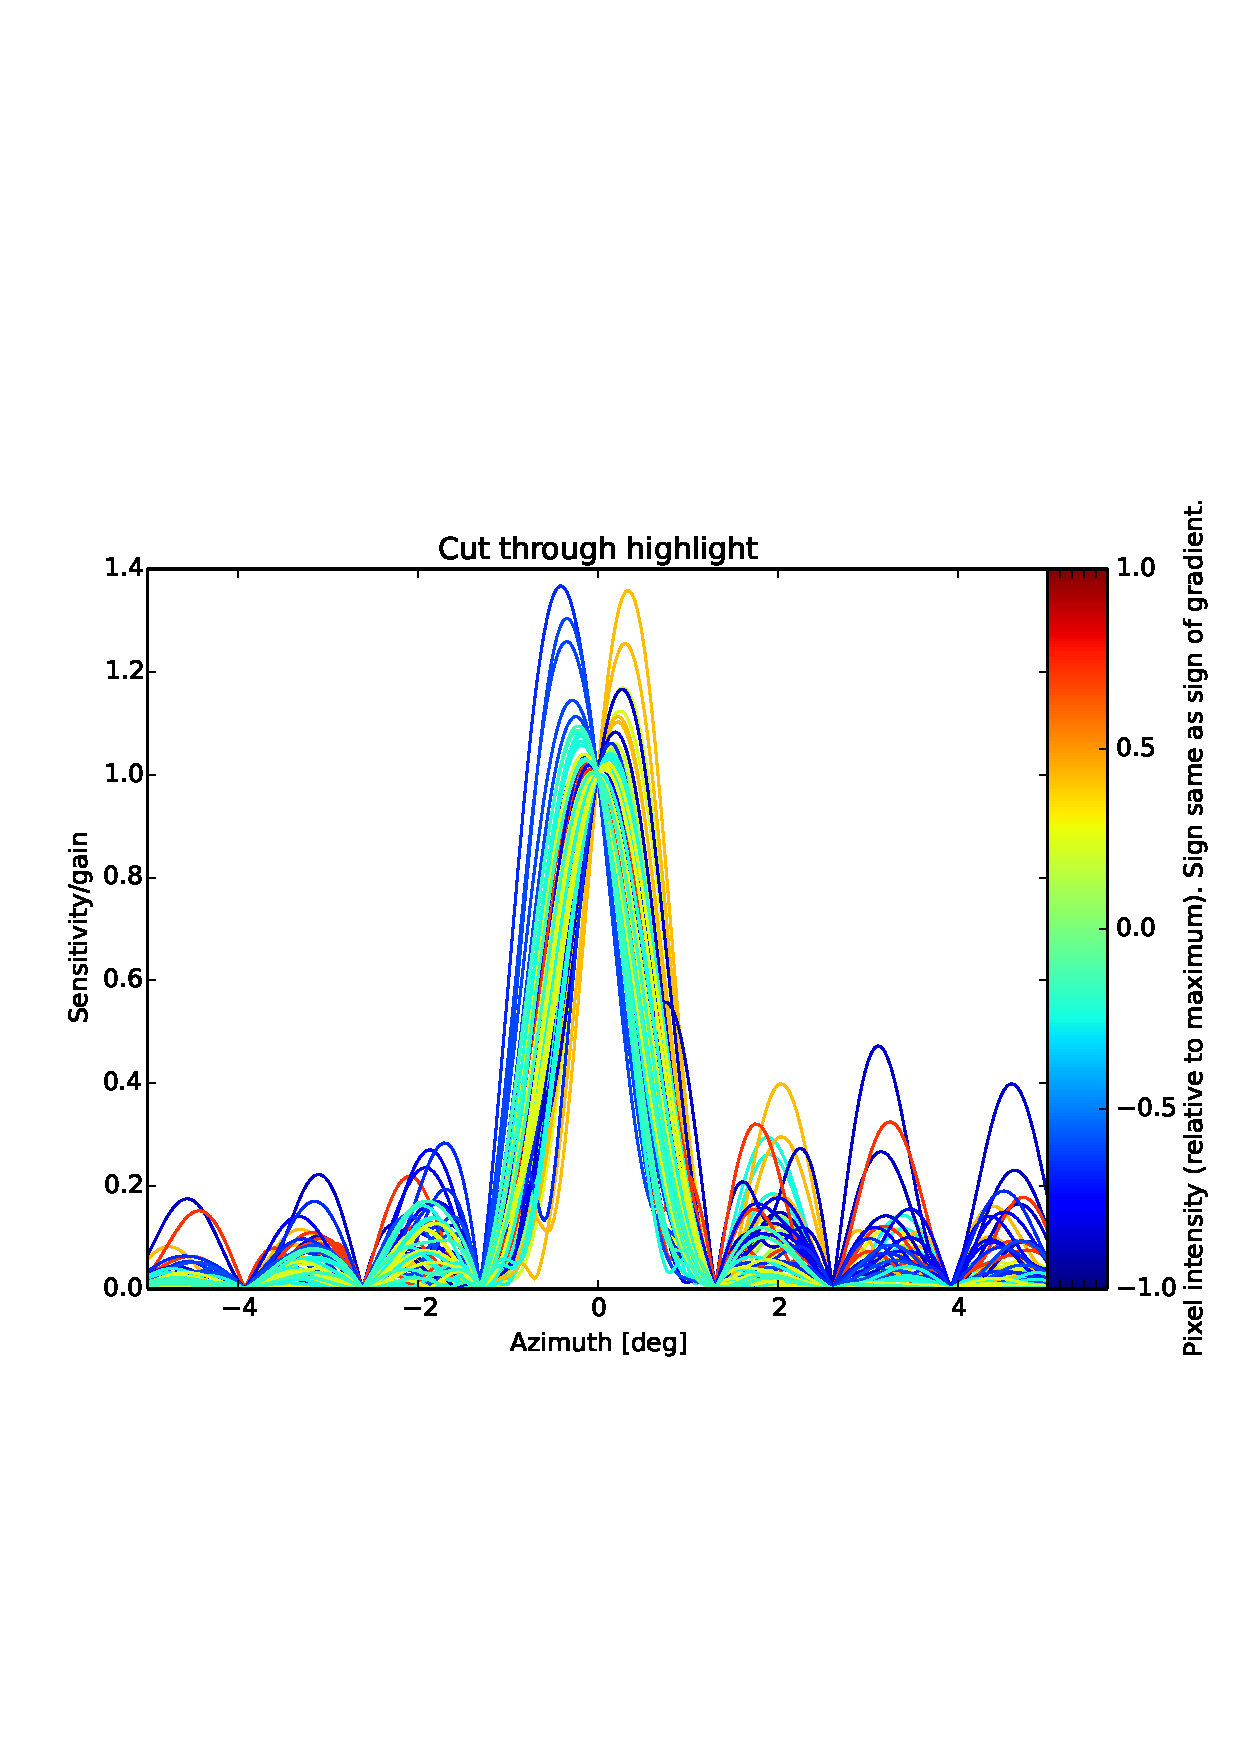
\includegraphics[width=0.49\linewidth]{gfx/1_win_resp_cut_highlight.png}}\\
\end{narrow}
\end{figure*}
\newpage
\begin{figure*}[!t]
\begin{narrow}{-1.2cm}{-1.2cm}\centering\vspace{-1.0cm}
\textbf{2. Capon: Tuning regularisation.}\\
\begin{tabular}[c]{l l l l}
\bf General & M = 32                            & $\Delta r = \frac{c}{2B}$ = 2.5 cm & $\frac{640\,\text{pixels}] / 12\,\text{m}}{\Delta r} = \frac{4}{3}$ \\
\bf LCA     & $\beta \in [0,10]$ (9 values) & $\phi \in [-1.07,1.07]$ deg (9 values) & Navg = 3 \\
\bf Capon   & $\Delta$ = 0.05                 & L = 16                           & Navg = 3 \\
\end{tabular}
\subfloat[LCA Window Response]{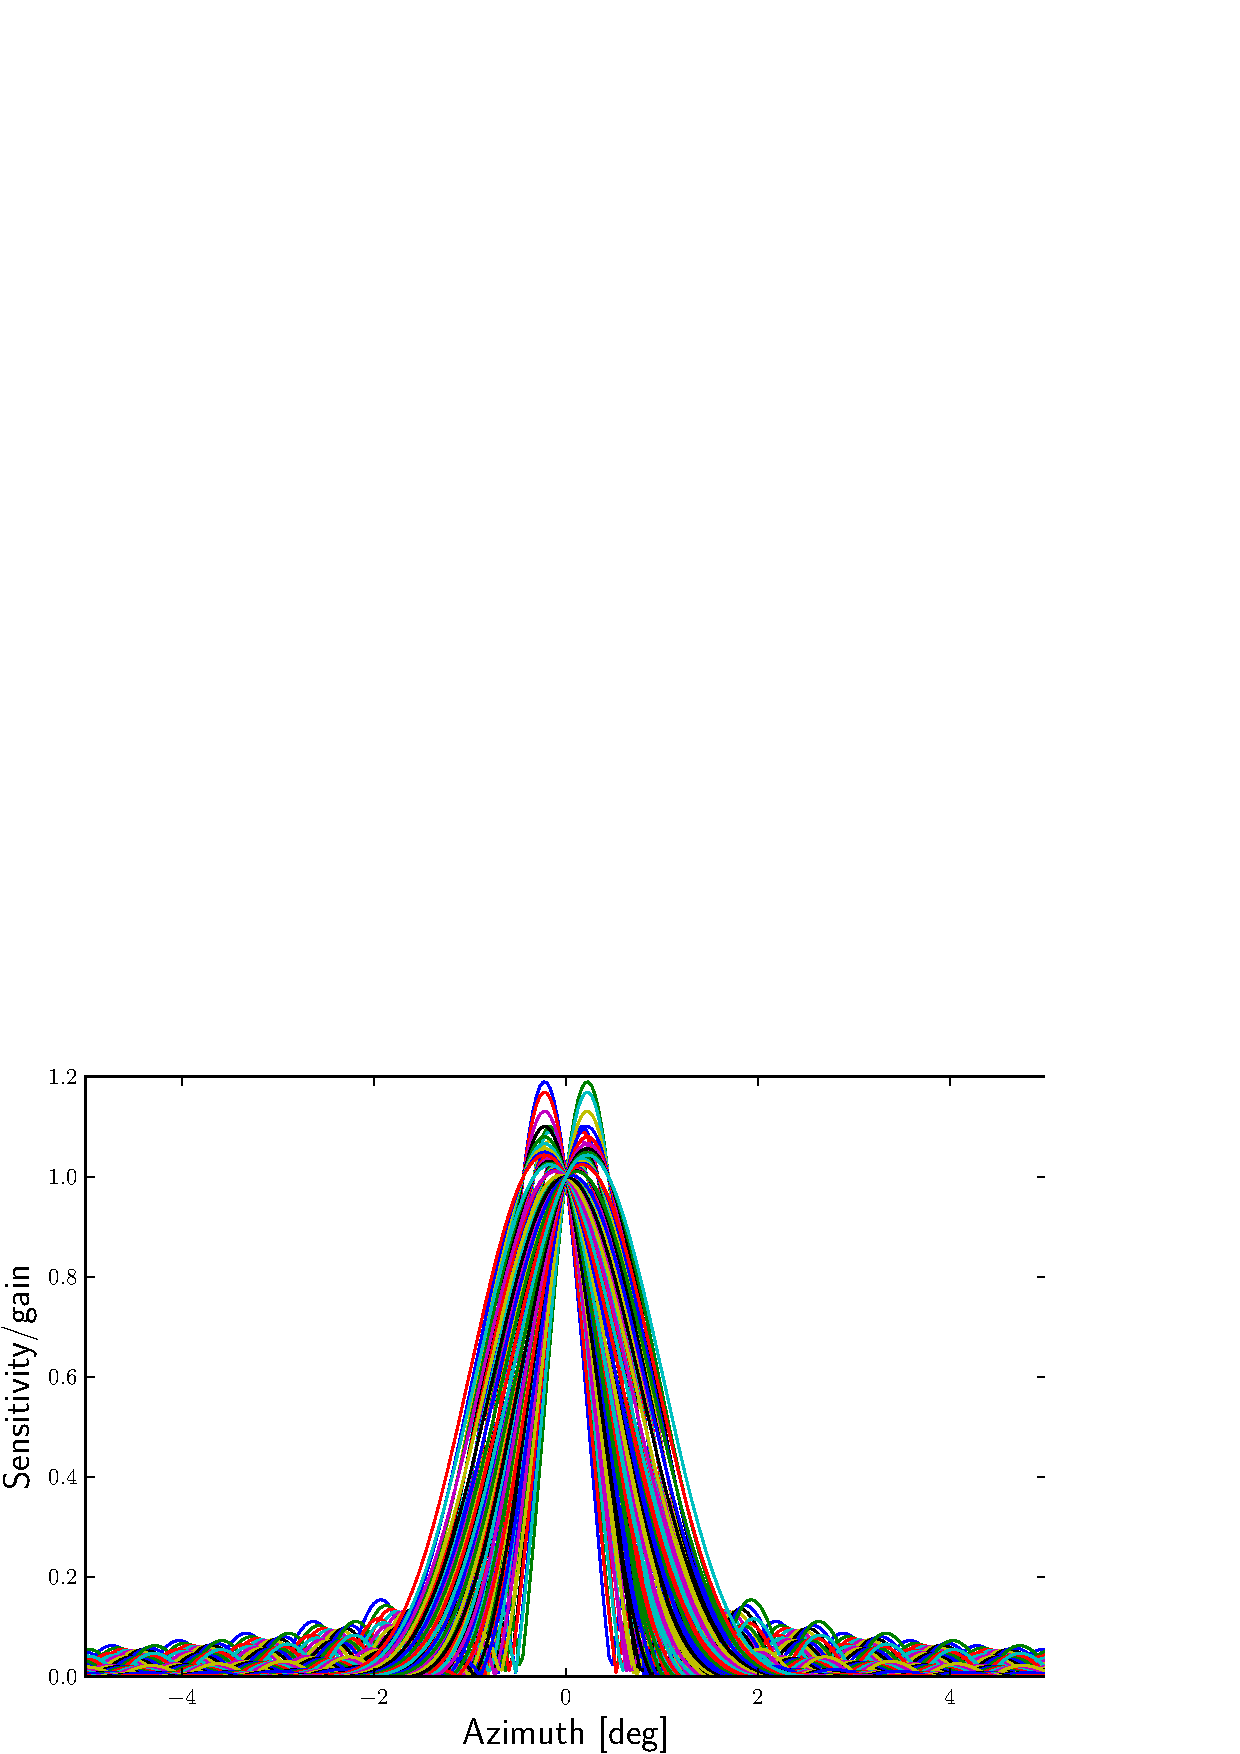
\includegraphics[width=0.49\linewidth]{gfx/2_window_response.png}}\hfill
\subfloat[Mean images]{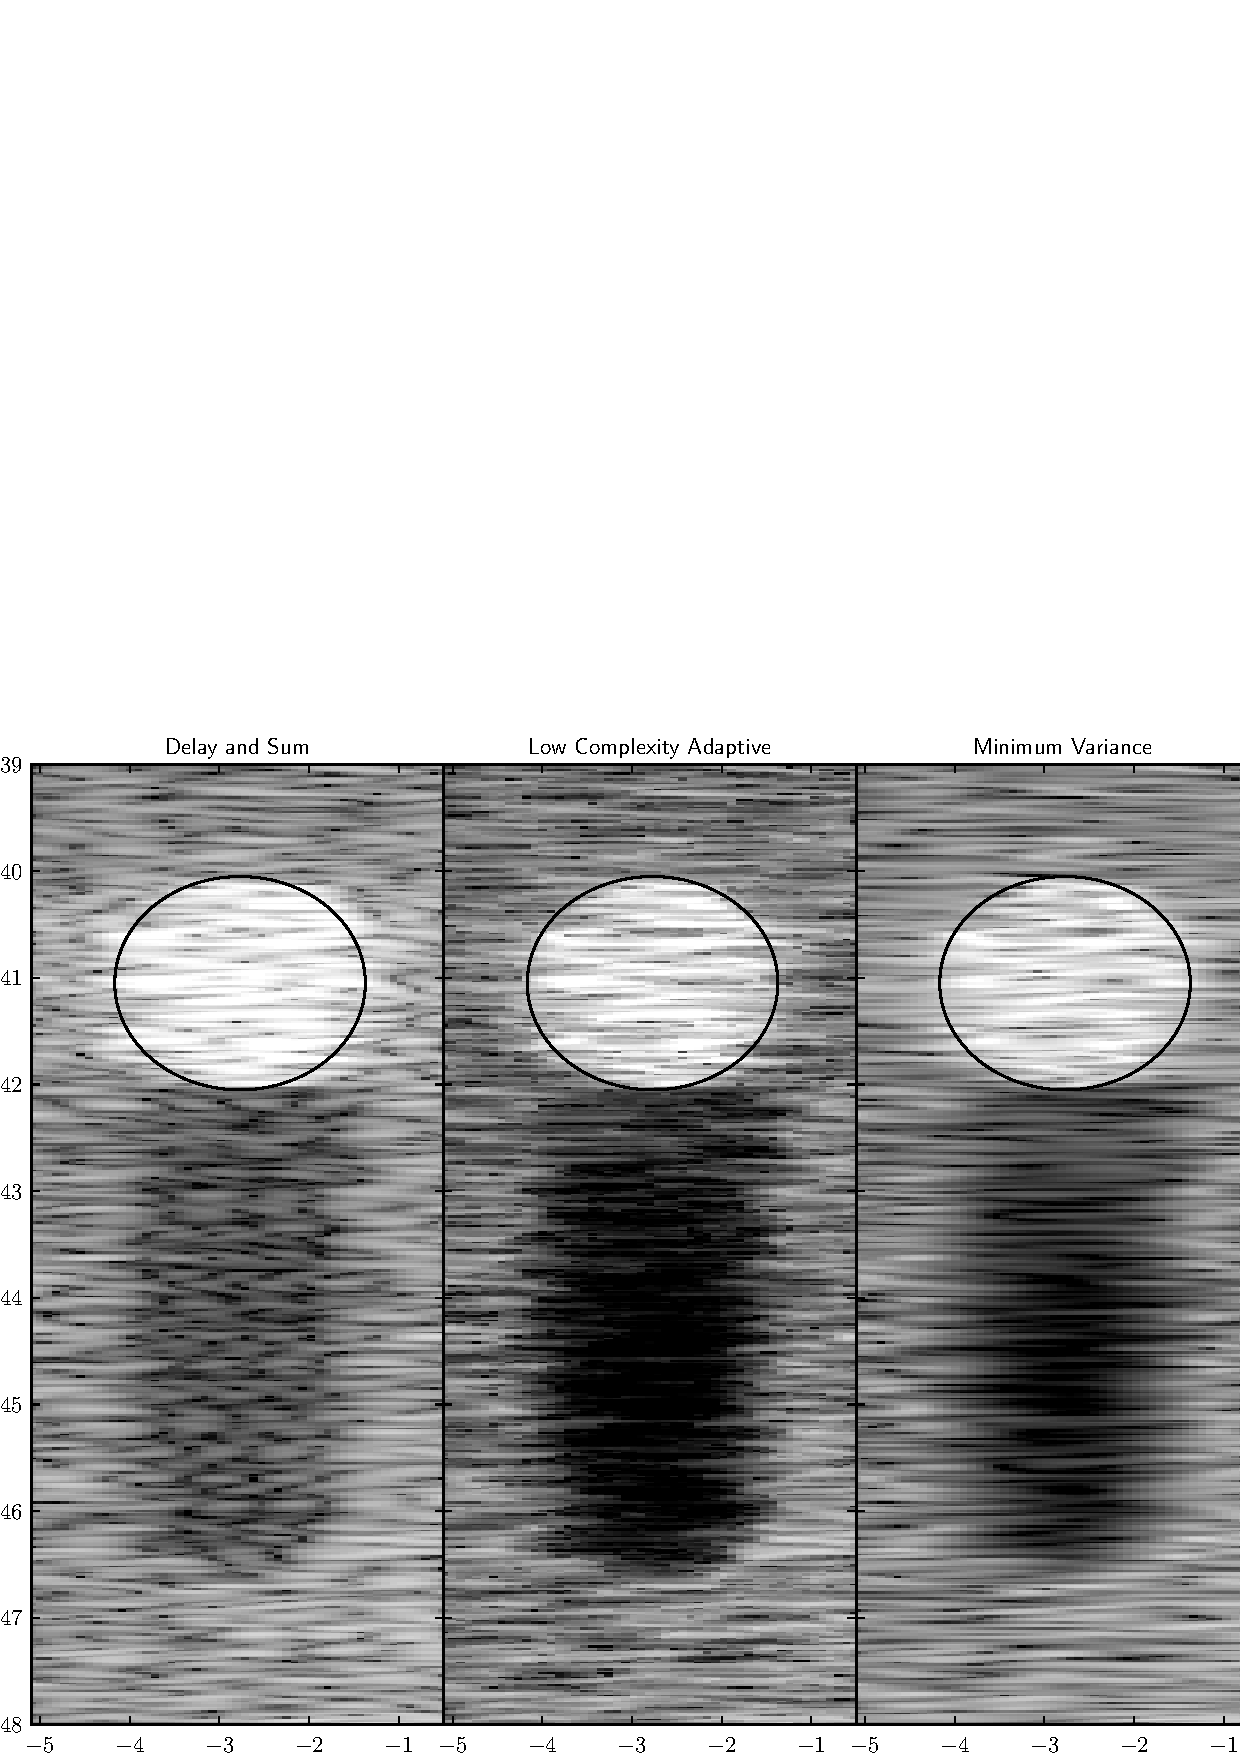
\includegraphics[width=0.49\linewidth]{gfx/2_mean_imgs.png}}\\
\subfloat[Windows ($\beta$)]{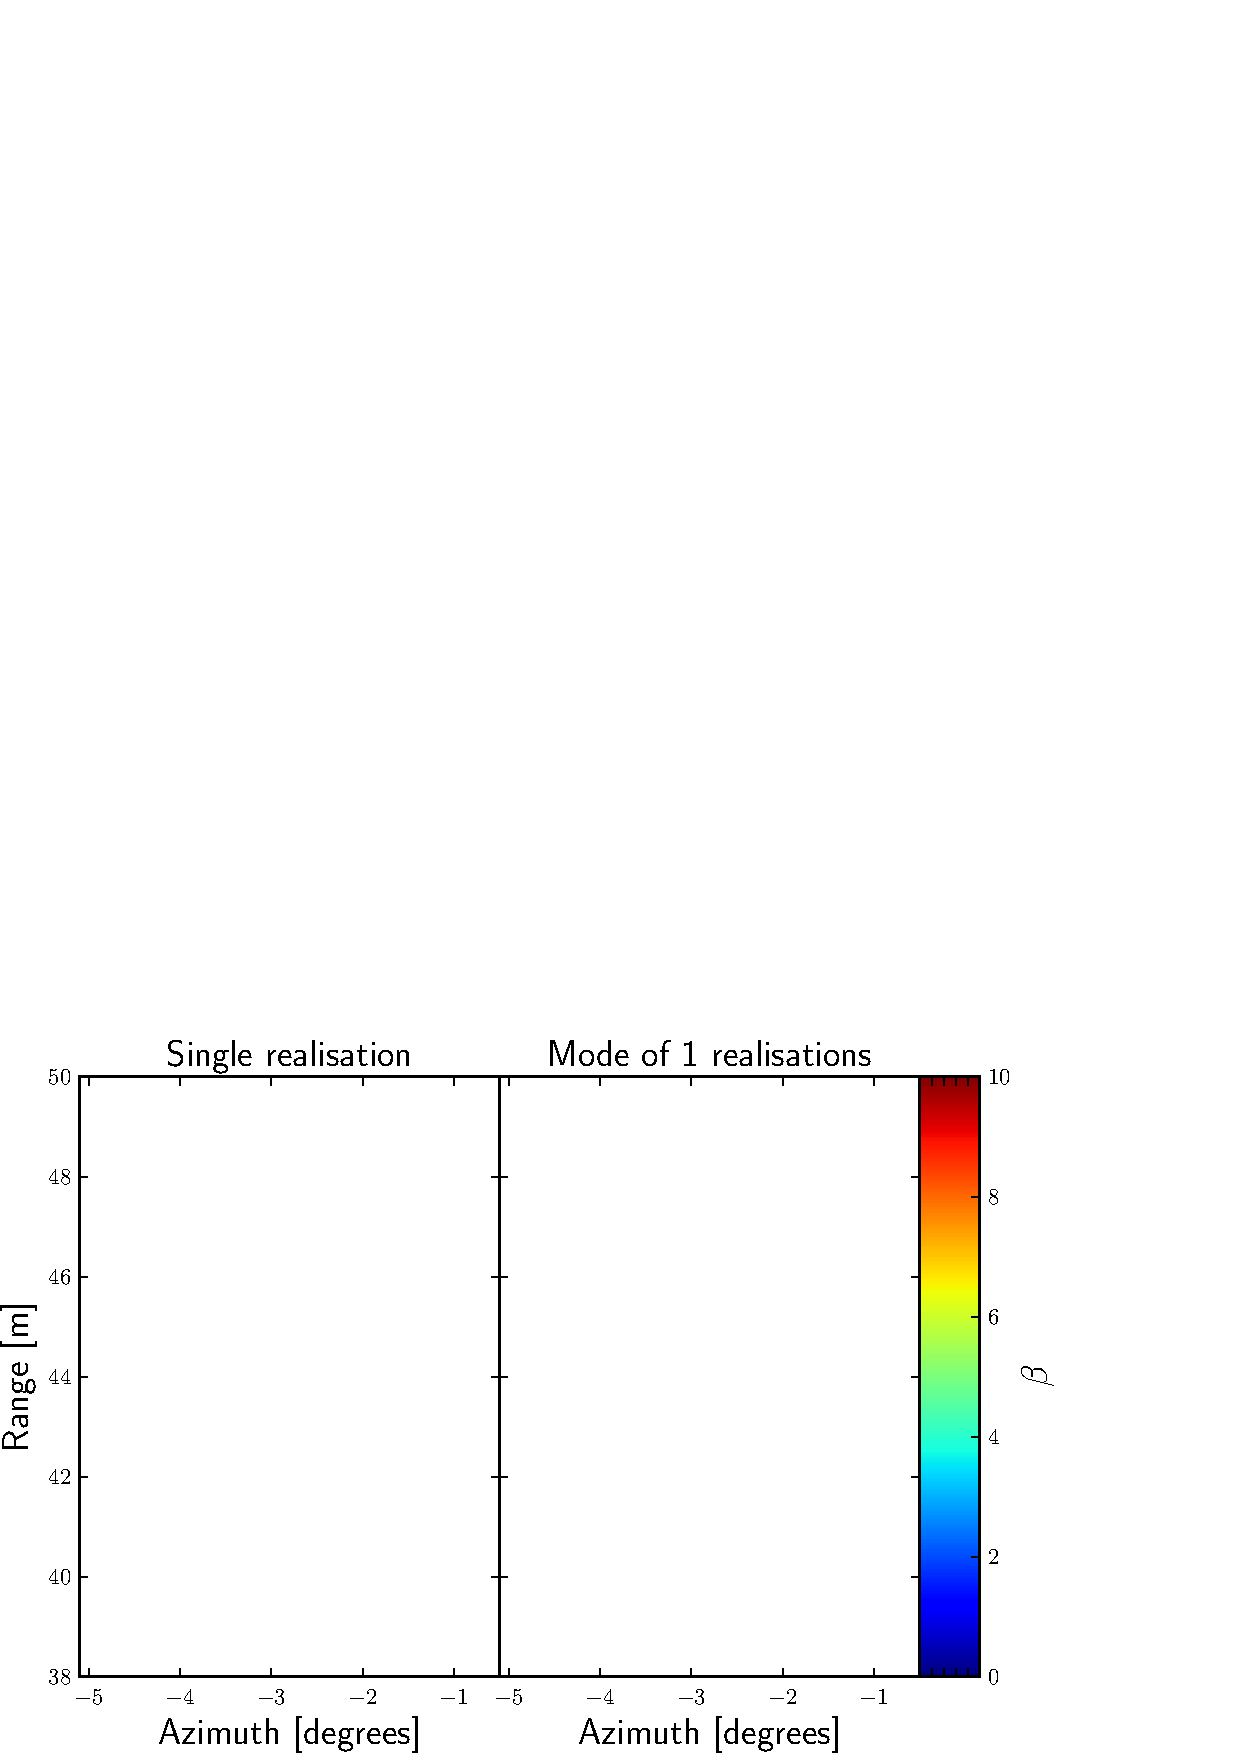
\includegraphics[width=0.49\linewidth]{gfx/2_windows_beta.png}}\hfill
\subfloat[Windows ($\phi$)]{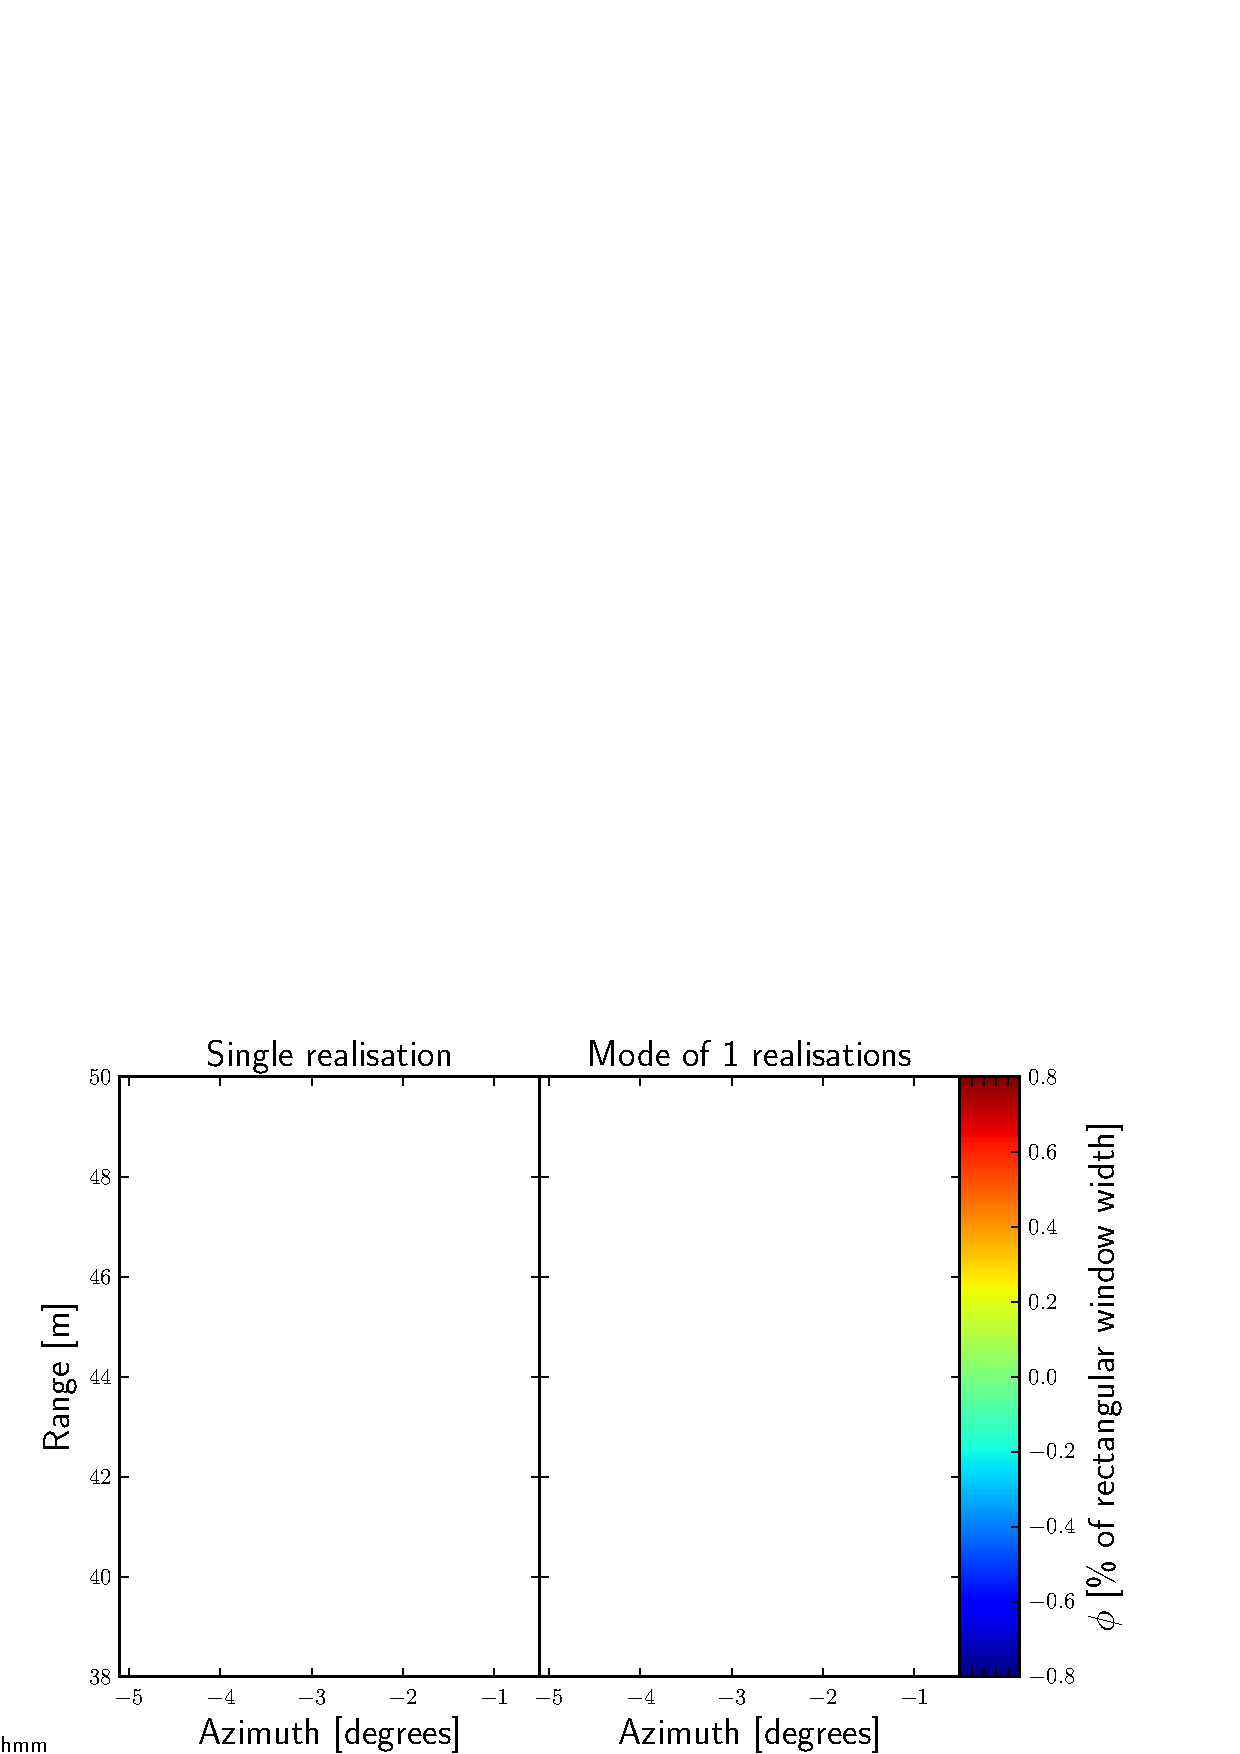
\includegraphics[width=0.48\linewidth]{gfx/2_windows_phi.png}}\\
\subfloat[Capon win. resp. through shadow]{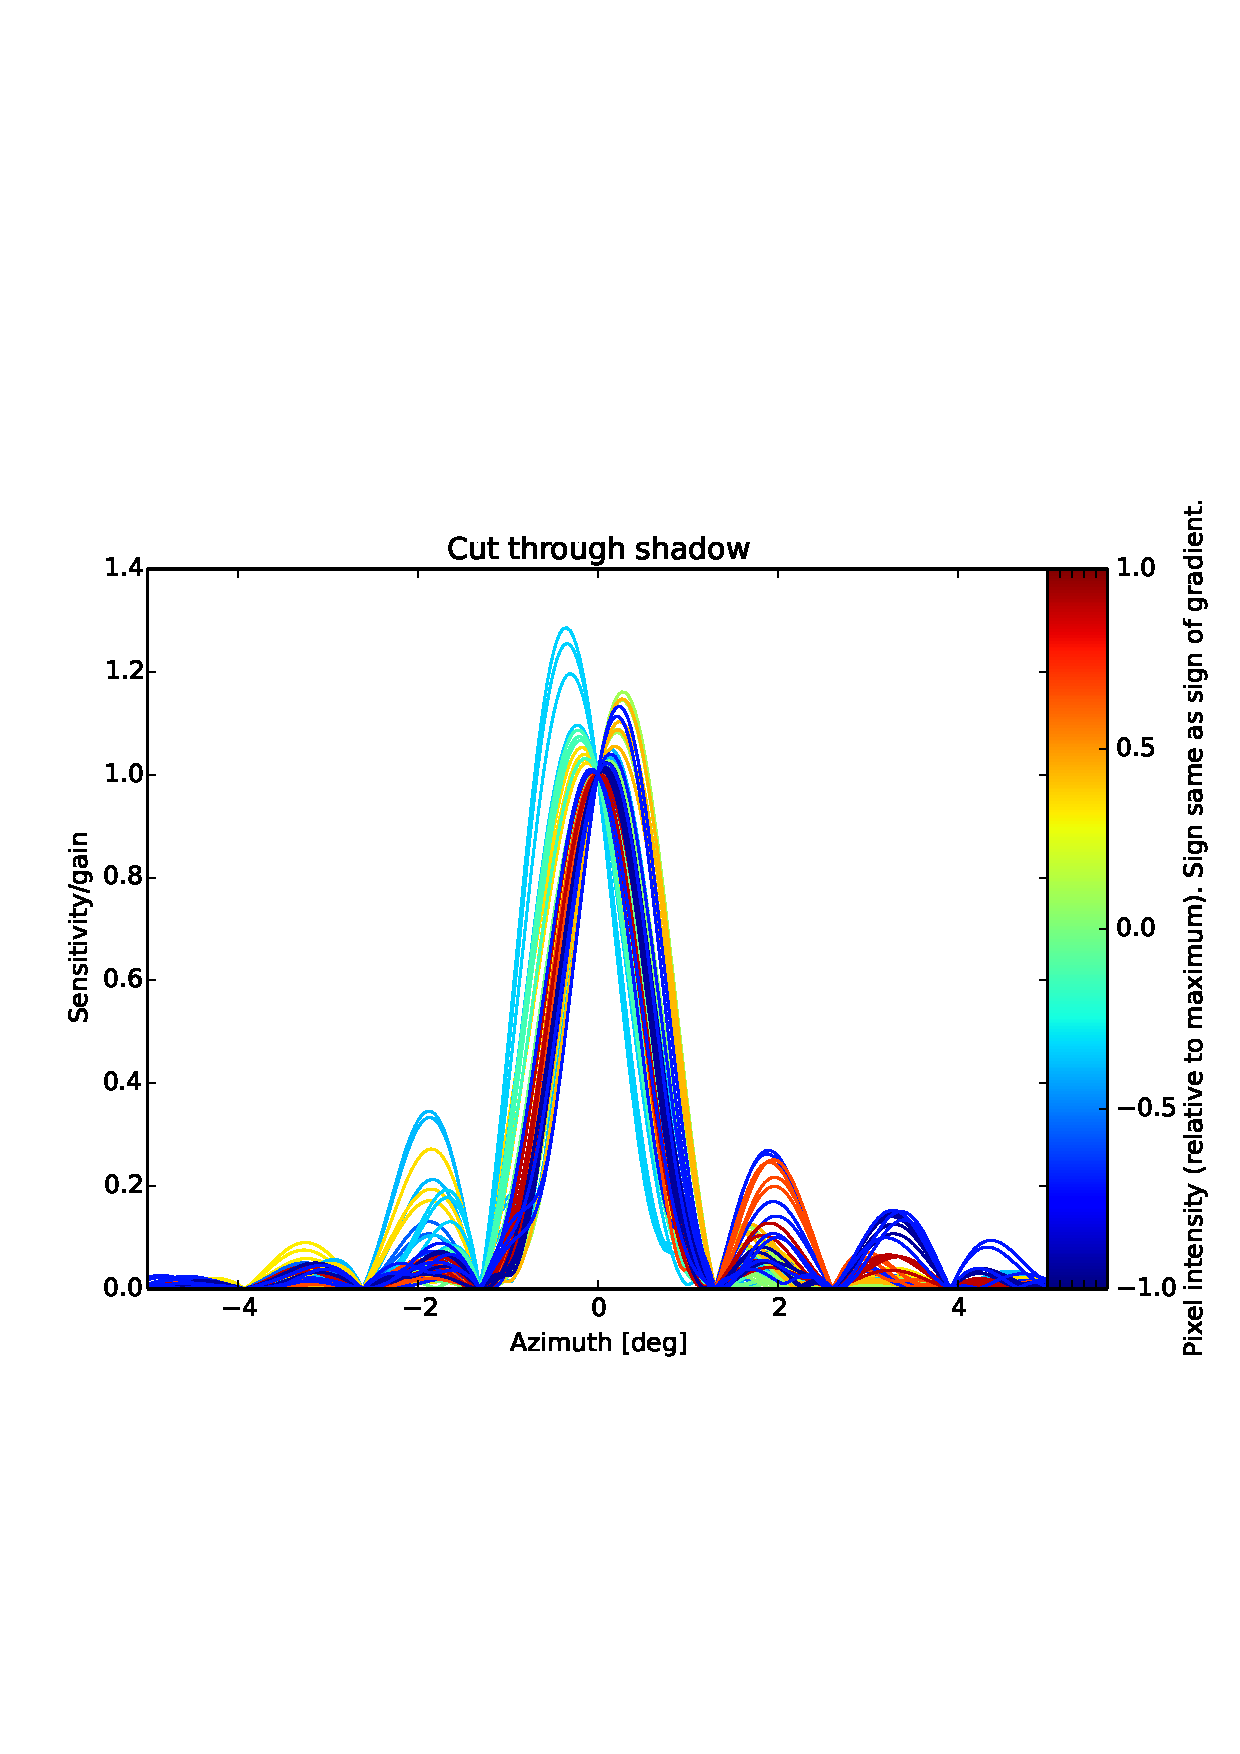
\includegraphics[width=0.49\linewidth]{gfx/2_win_resp_cut_shadow.png}}\hfill
\subfloat[Capon win. resp. through highlight]{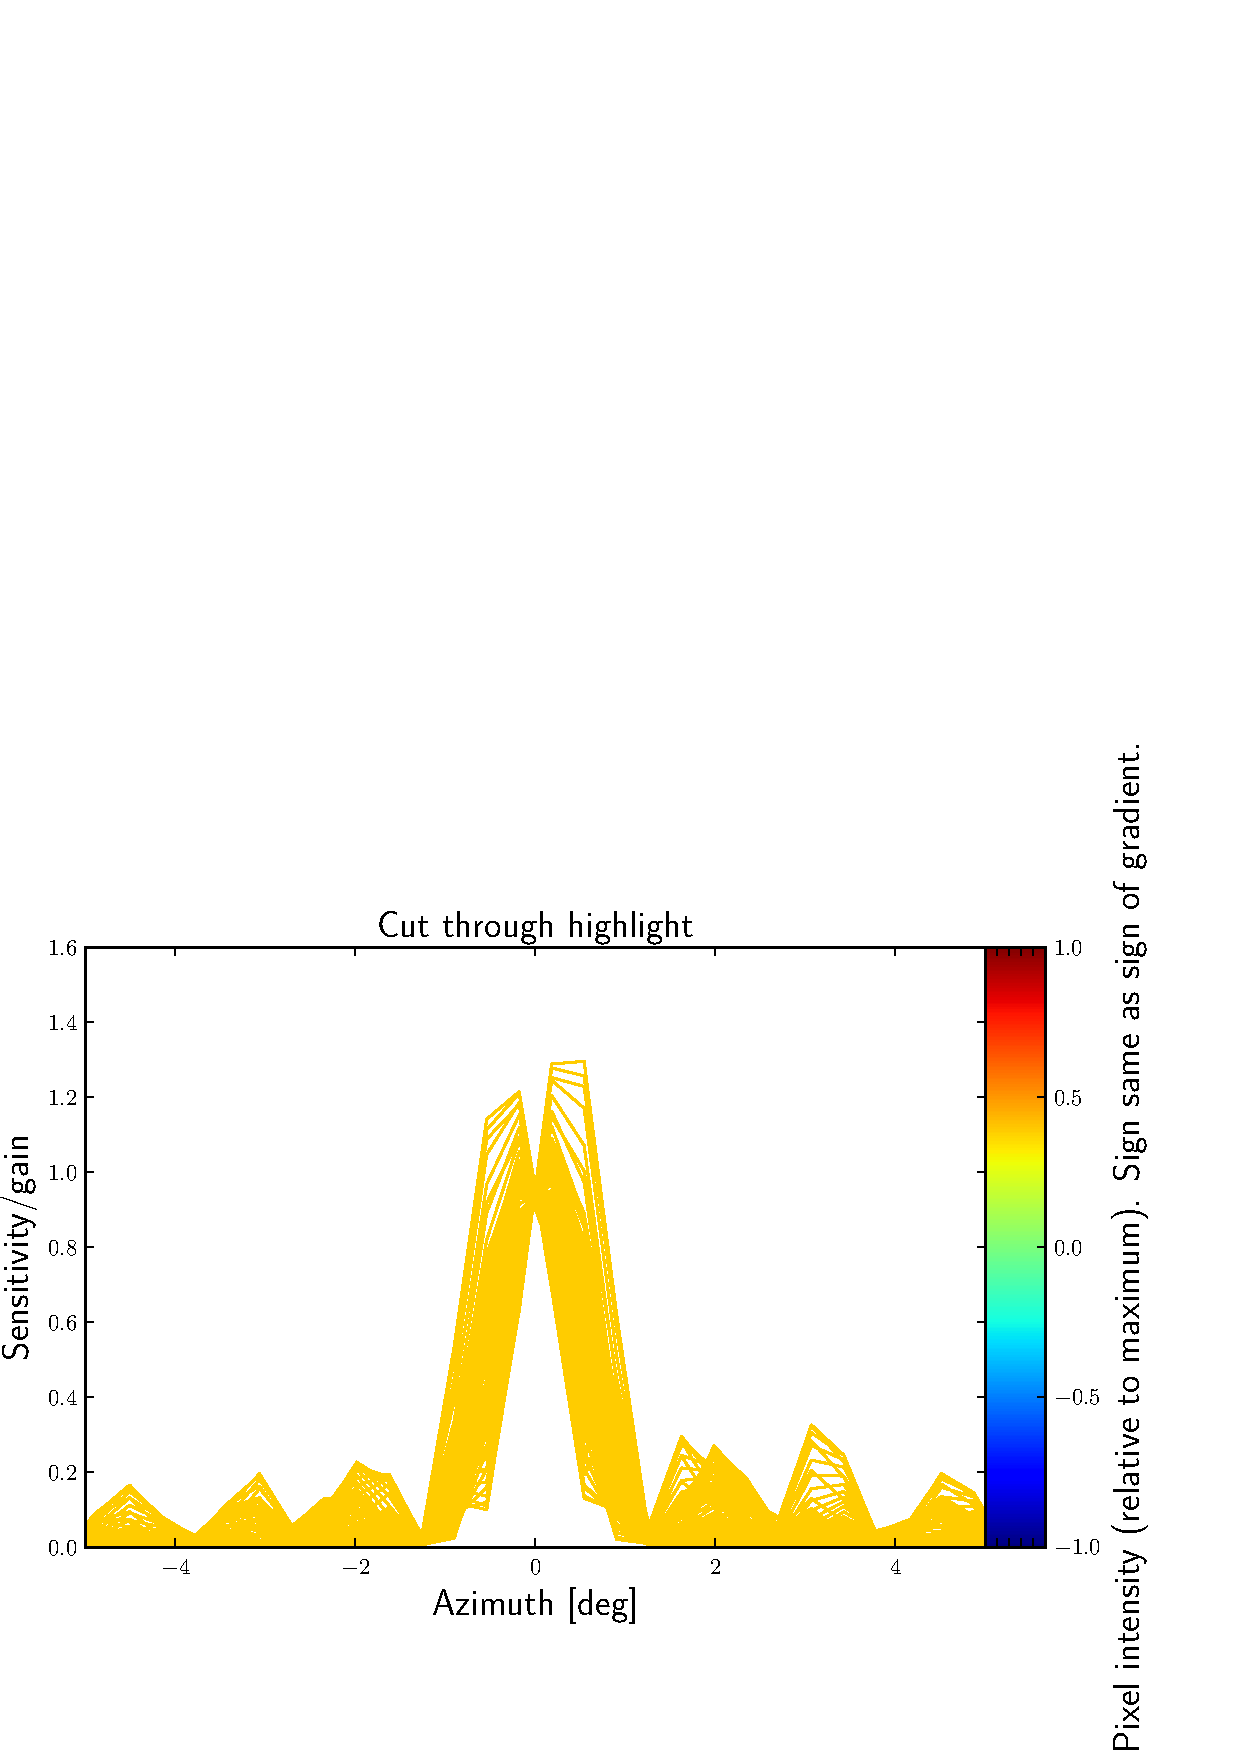
\includegraphics[width=0.49\linewidth]{gfx/2_win_resp_cut_highlight.png}}\\
\end{narrow}
\end{figure*}
\newpage
\begin{figure*}[!t]
\begin{narrow}{-1.2cm}{-1.2cm}\centering\vspace{-1.0cm}
\textbf{3. Capon: Tuning regularisation.}\\
\begin{tabular}[c]{l l l l}
\bf General & M = 32                            & $\Delta r = \frac{c}{2B}$ = 2.5 cm & $\frac{640\,\text{pixels}] / 12\,\text{m}}{\Delta r} = \frac{4}{3}$ \\
\bf LCA     & $\beta \in [0,10]$ (9 values) & $\phi \in [-1.07,1.07]$ deg (9 values) & Navg = 3 \\
\bf Capon   & $\Delta$ = 0.20                 & L = 16                           & Navg = 3 \\
\end{tabular}
\subfloat[LCA Window Response]{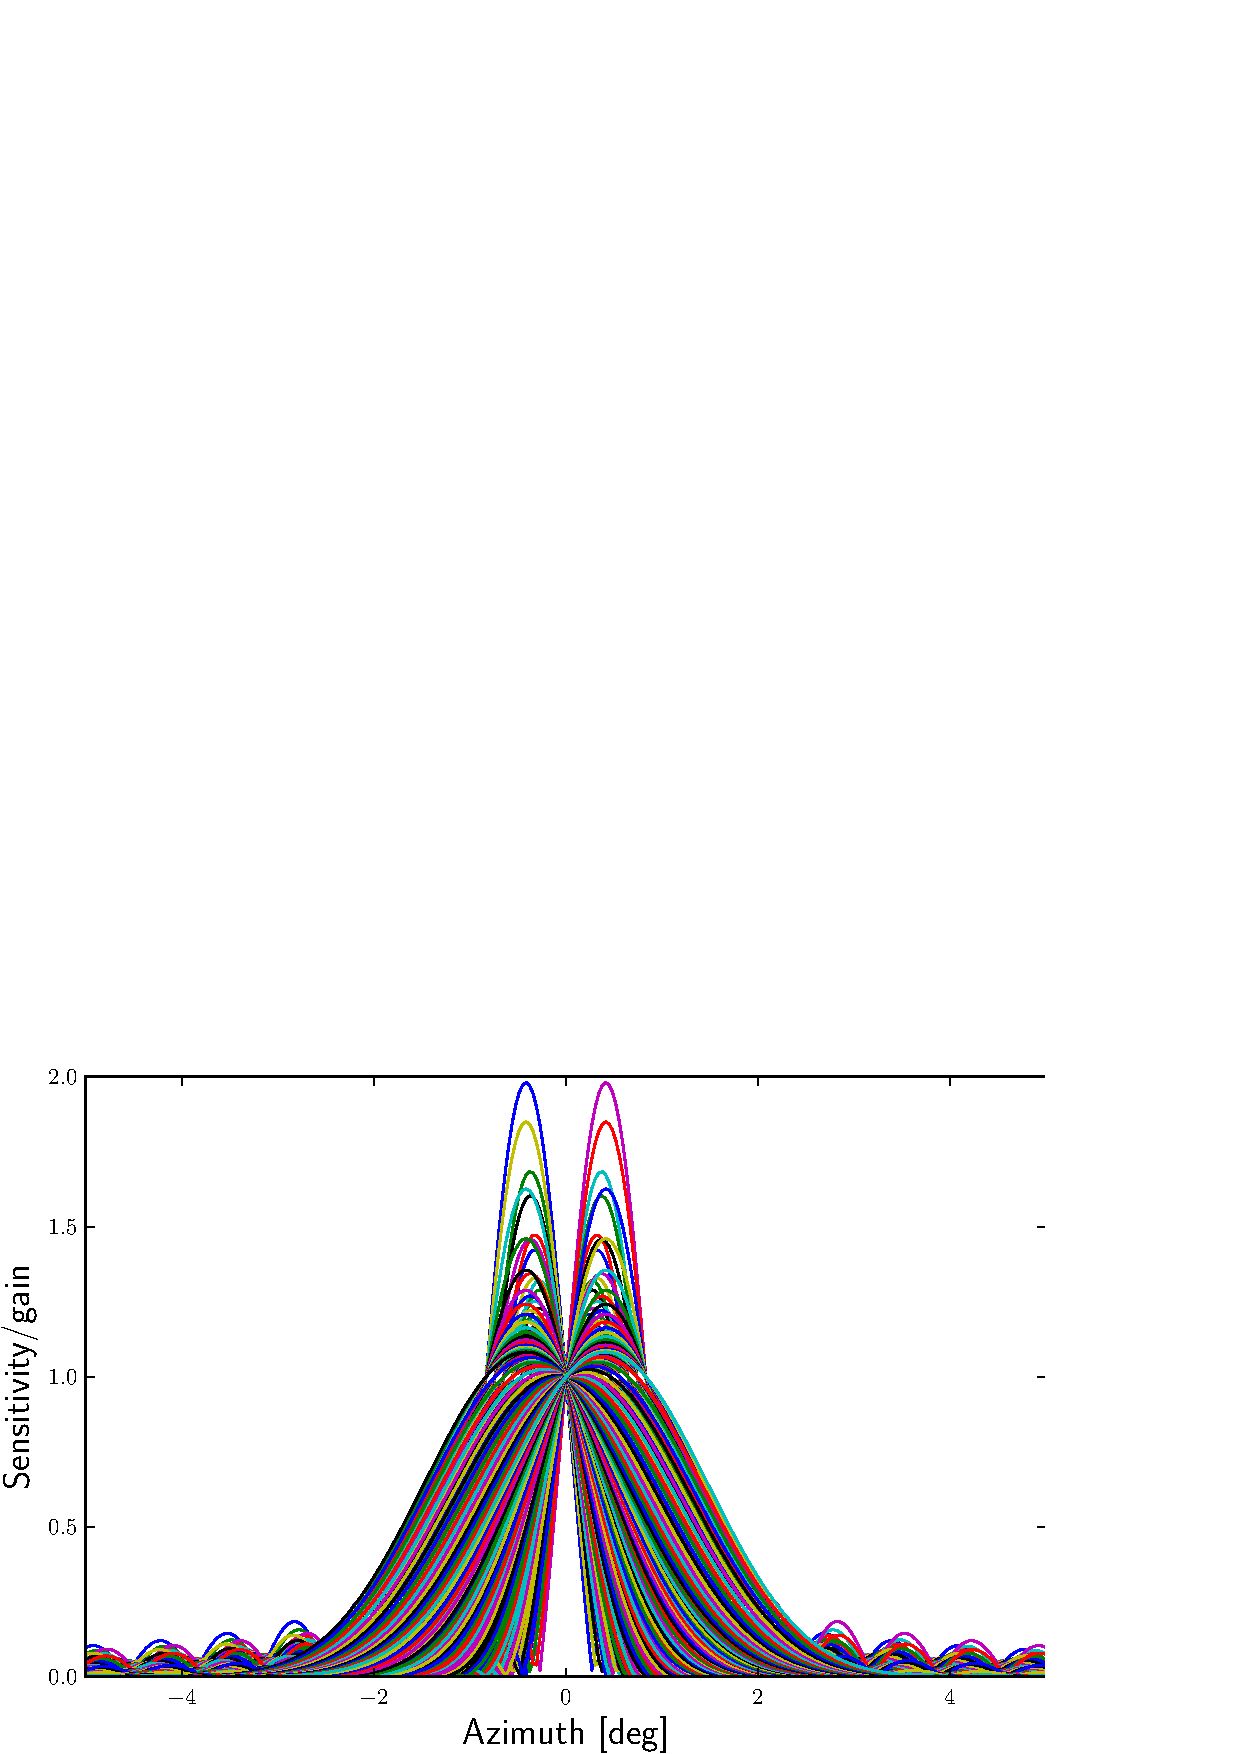
\includegraphics[width=0.49\linewidth]{gfx/3_window_response.png}}\hfill
\subfloat[Mean images]{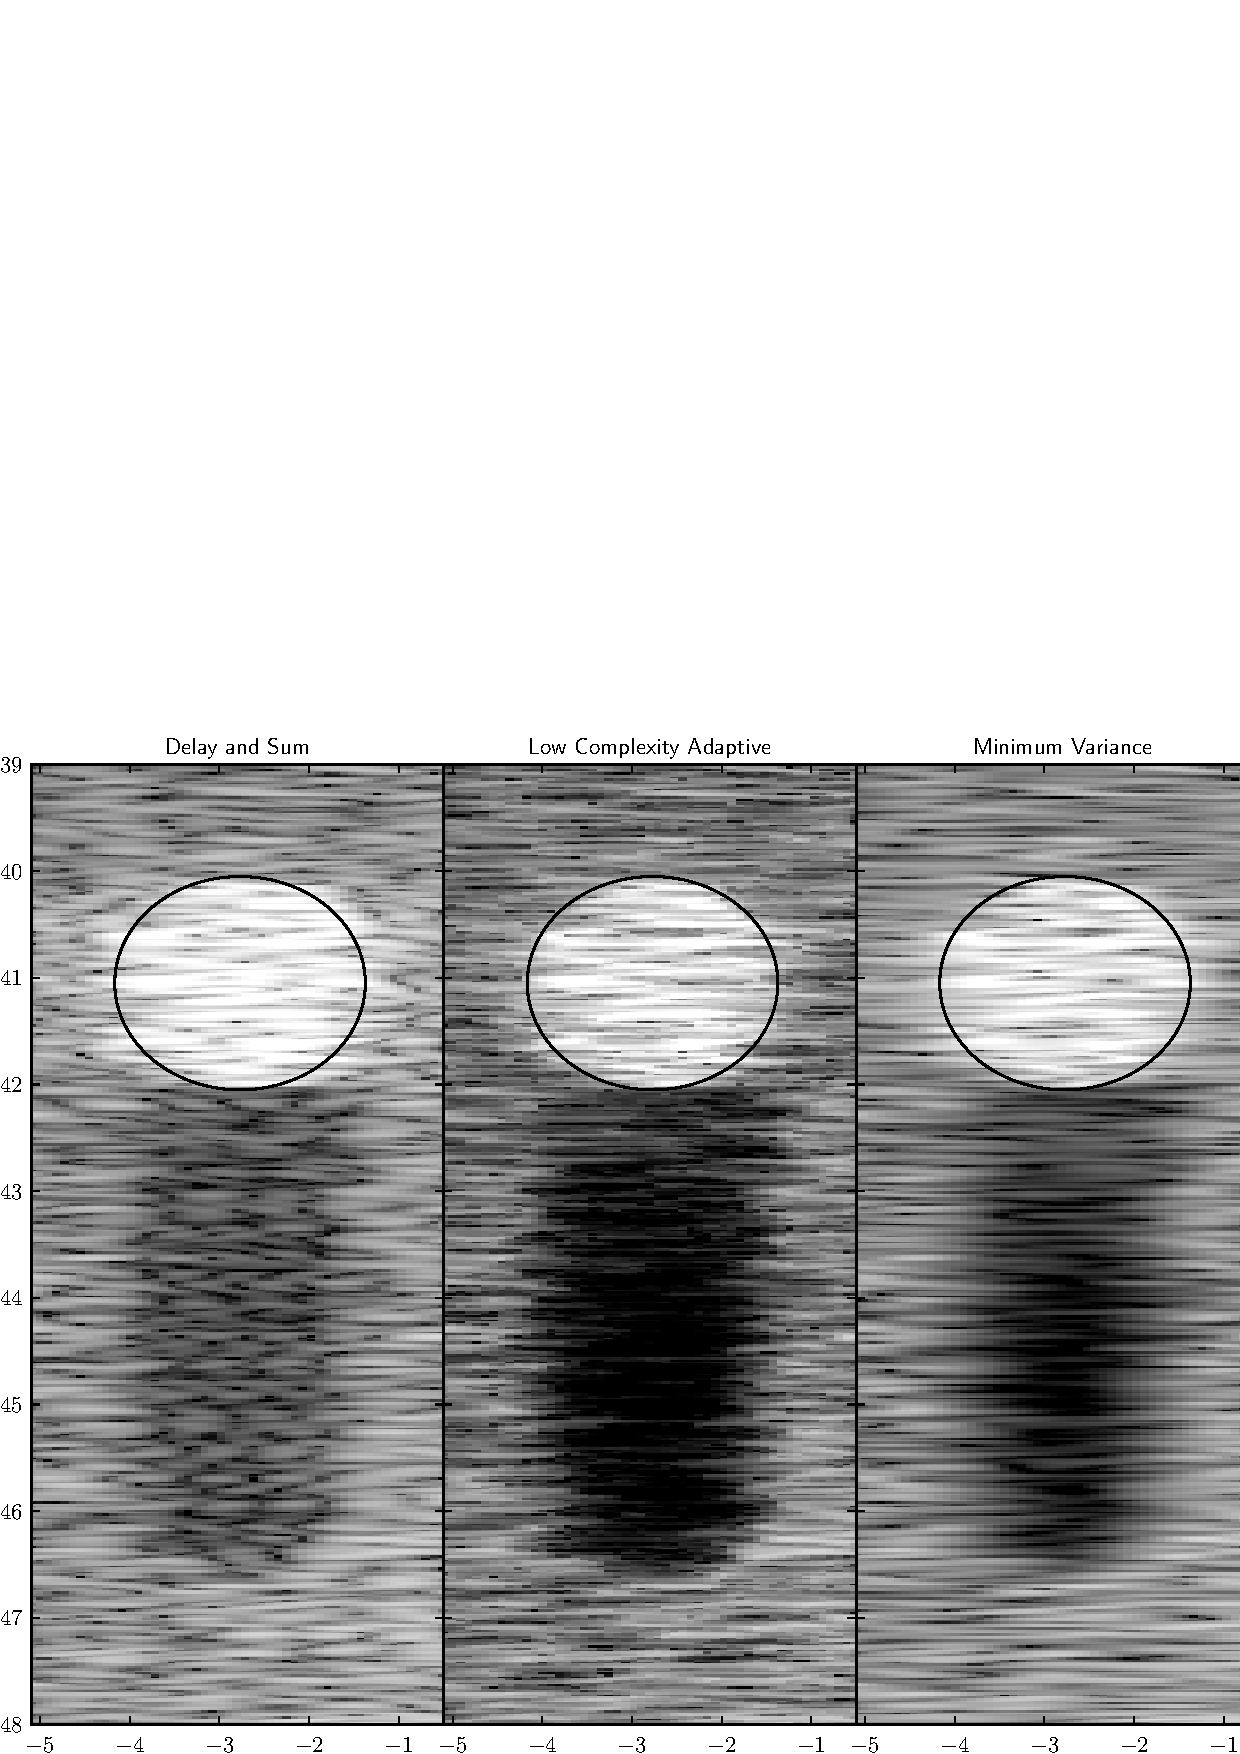
\includegraphics[width=0.49\linewidth]{gfx/3_mean_imgs.png}}\\
\subfloat[Windows ($\beta$)]{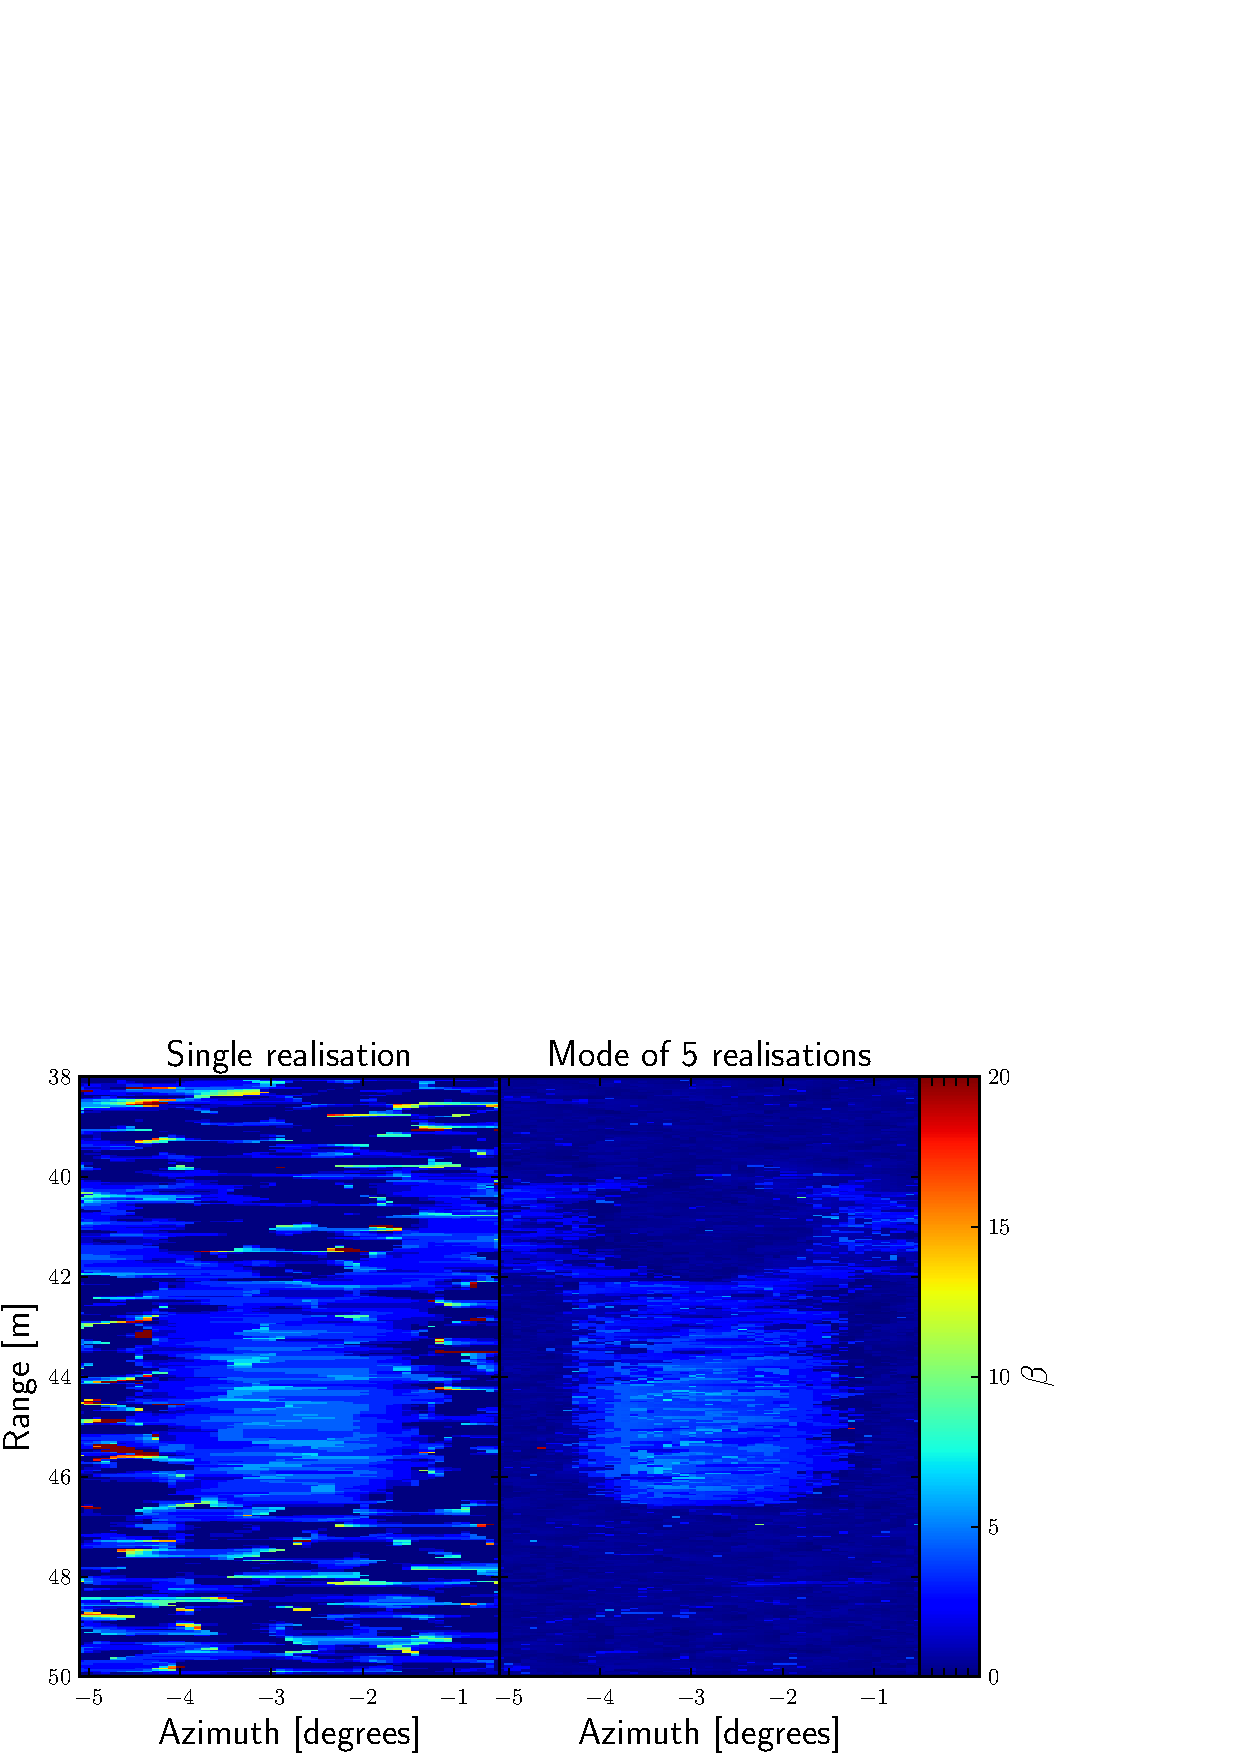
\includegraphics[width=0.49\linewidth]{gfx/3_windows_beta.png}}\hfill
\subfloat[Windows ($\phi$)]{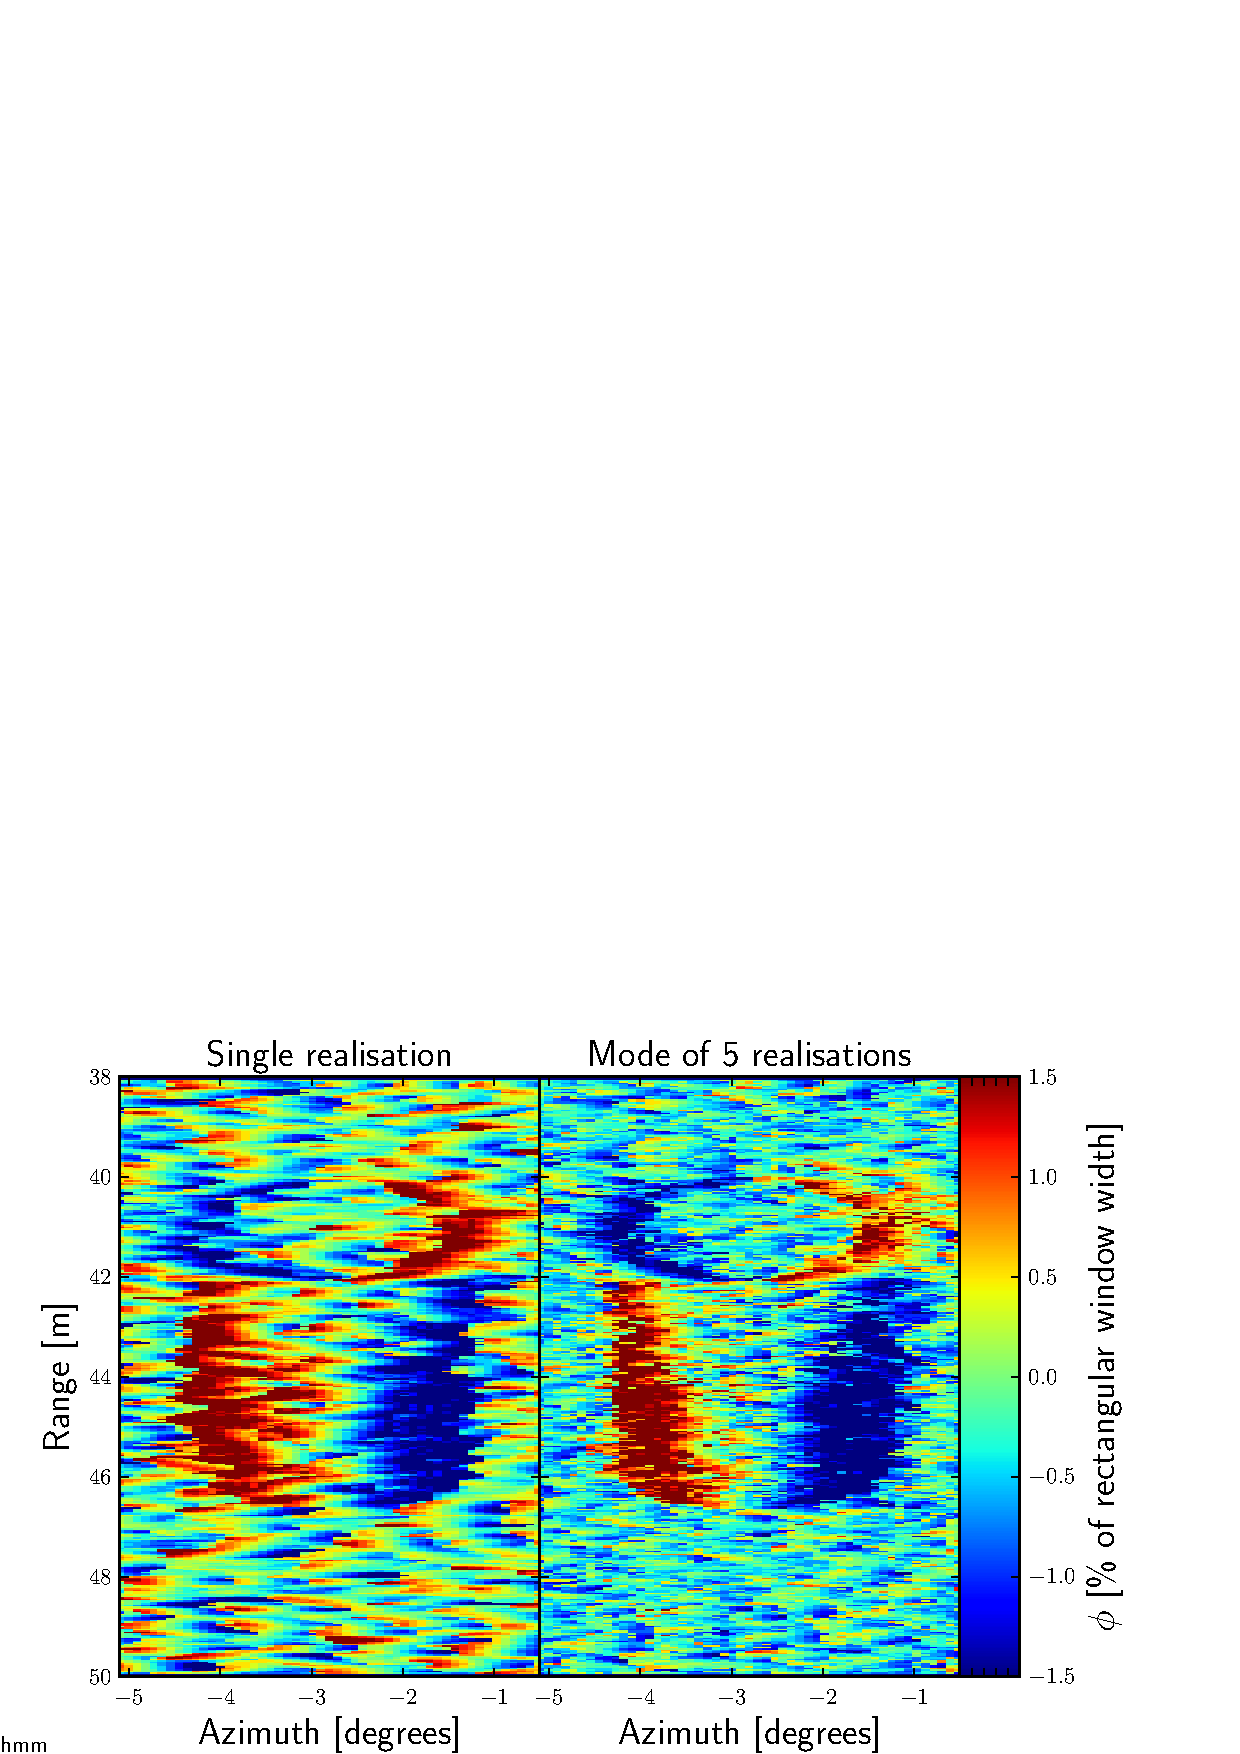
\includegraphics[width=0.48\linewidth]{gfx/3_windows_phi.png}}\\
\subfloat[Capon win. resp. through shadow]{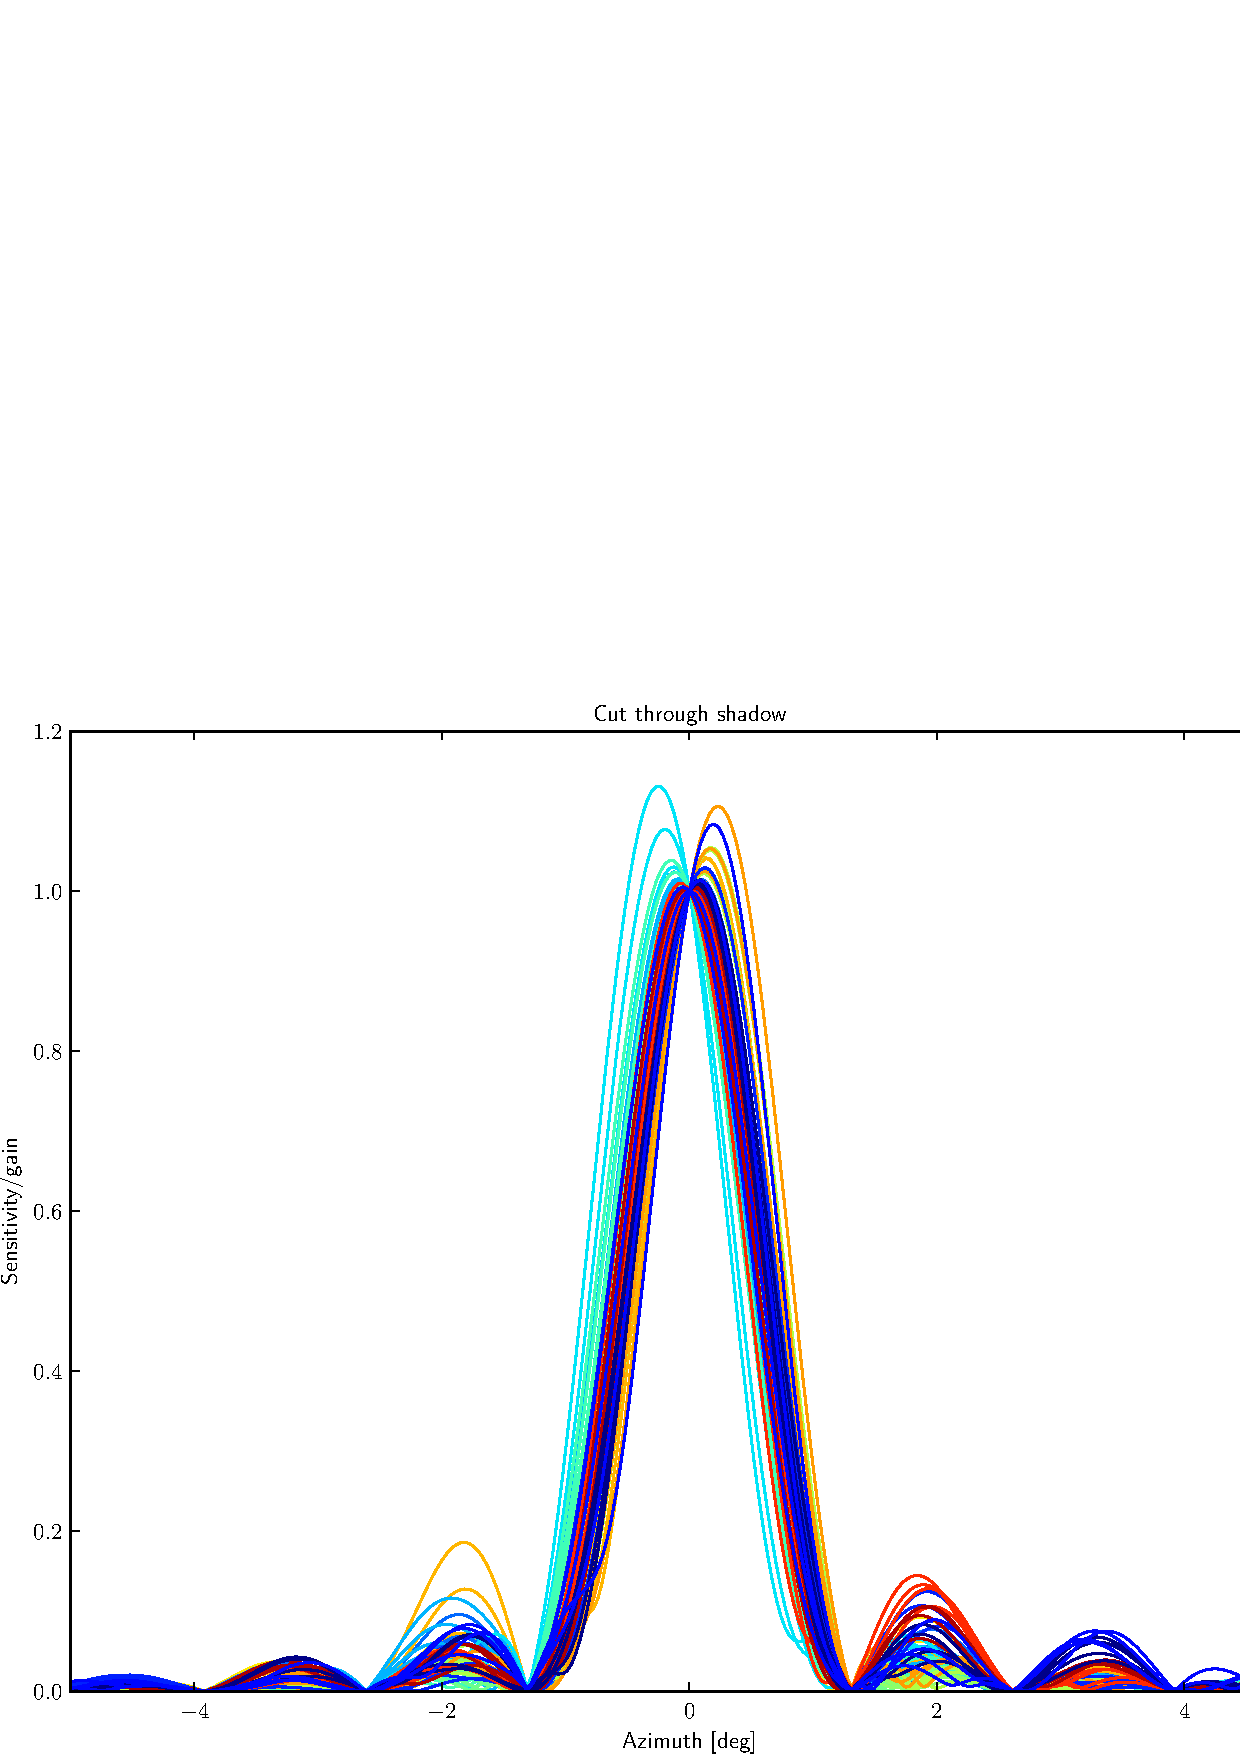
\includegraphics[width=0.49\linewidth]{gfx/3_win_resp_cut_shadow.png}}\hfill
\subfloat[Capon win. resp. through highlight]{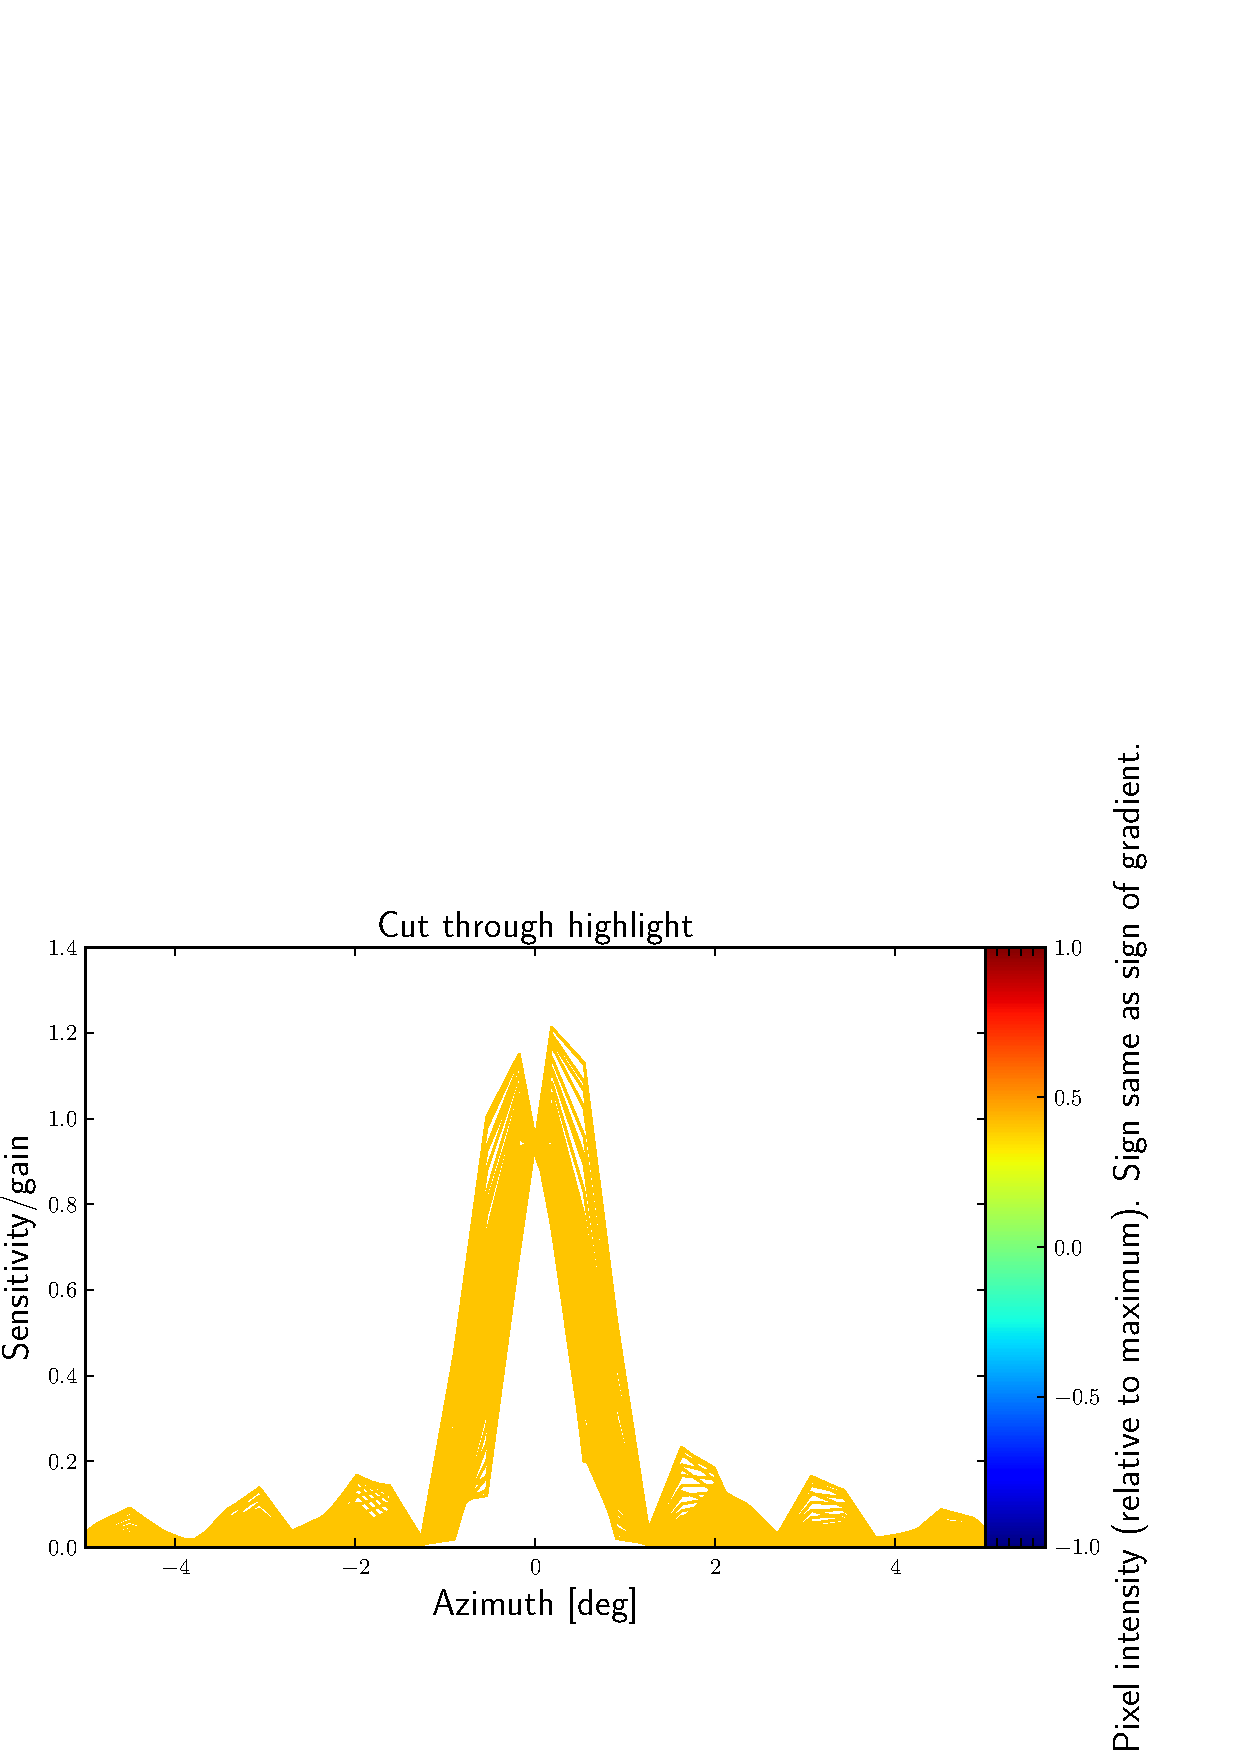
\includegraphics[width=0.49\linewidth]{gfx/3_win_resp_cut_highlight.png}}\\
\end{narrow}
\end{figure*}
\newpage
\begin{figure*}[!t]
\begin{narrow}{-1.2cm}{-1.2cm}\centering\vspace{-1.0cm}
\textbf{4. Capon: Tuning subarray.}\\
\begin{tabular}[c]{l l l l}
\bf General & M = 32                            & $\Delta r = \frac{c}{2B}$ = 2.5 cm & $\frac{640\,\text{pixels}] / 12\,\text{m}}{\Delta r} = \frac{4}{3}$ \\
\bf LCA     & $\beta \in [0,10]$ (9 values) & $\phi \in [-1.07,1.07]$ deg (9 values) & Navg = 3 \\
\bf Capon   & $\Delta$ = 0.01                 & L = 20                           & Navg = 3 \\
\end{tabular}
\subfloat[LCA Window Response]{\includegraphics[width=0.49\linewidth]{gfx/4_window_response.png}}\hfill
\subfloat[Mean images]{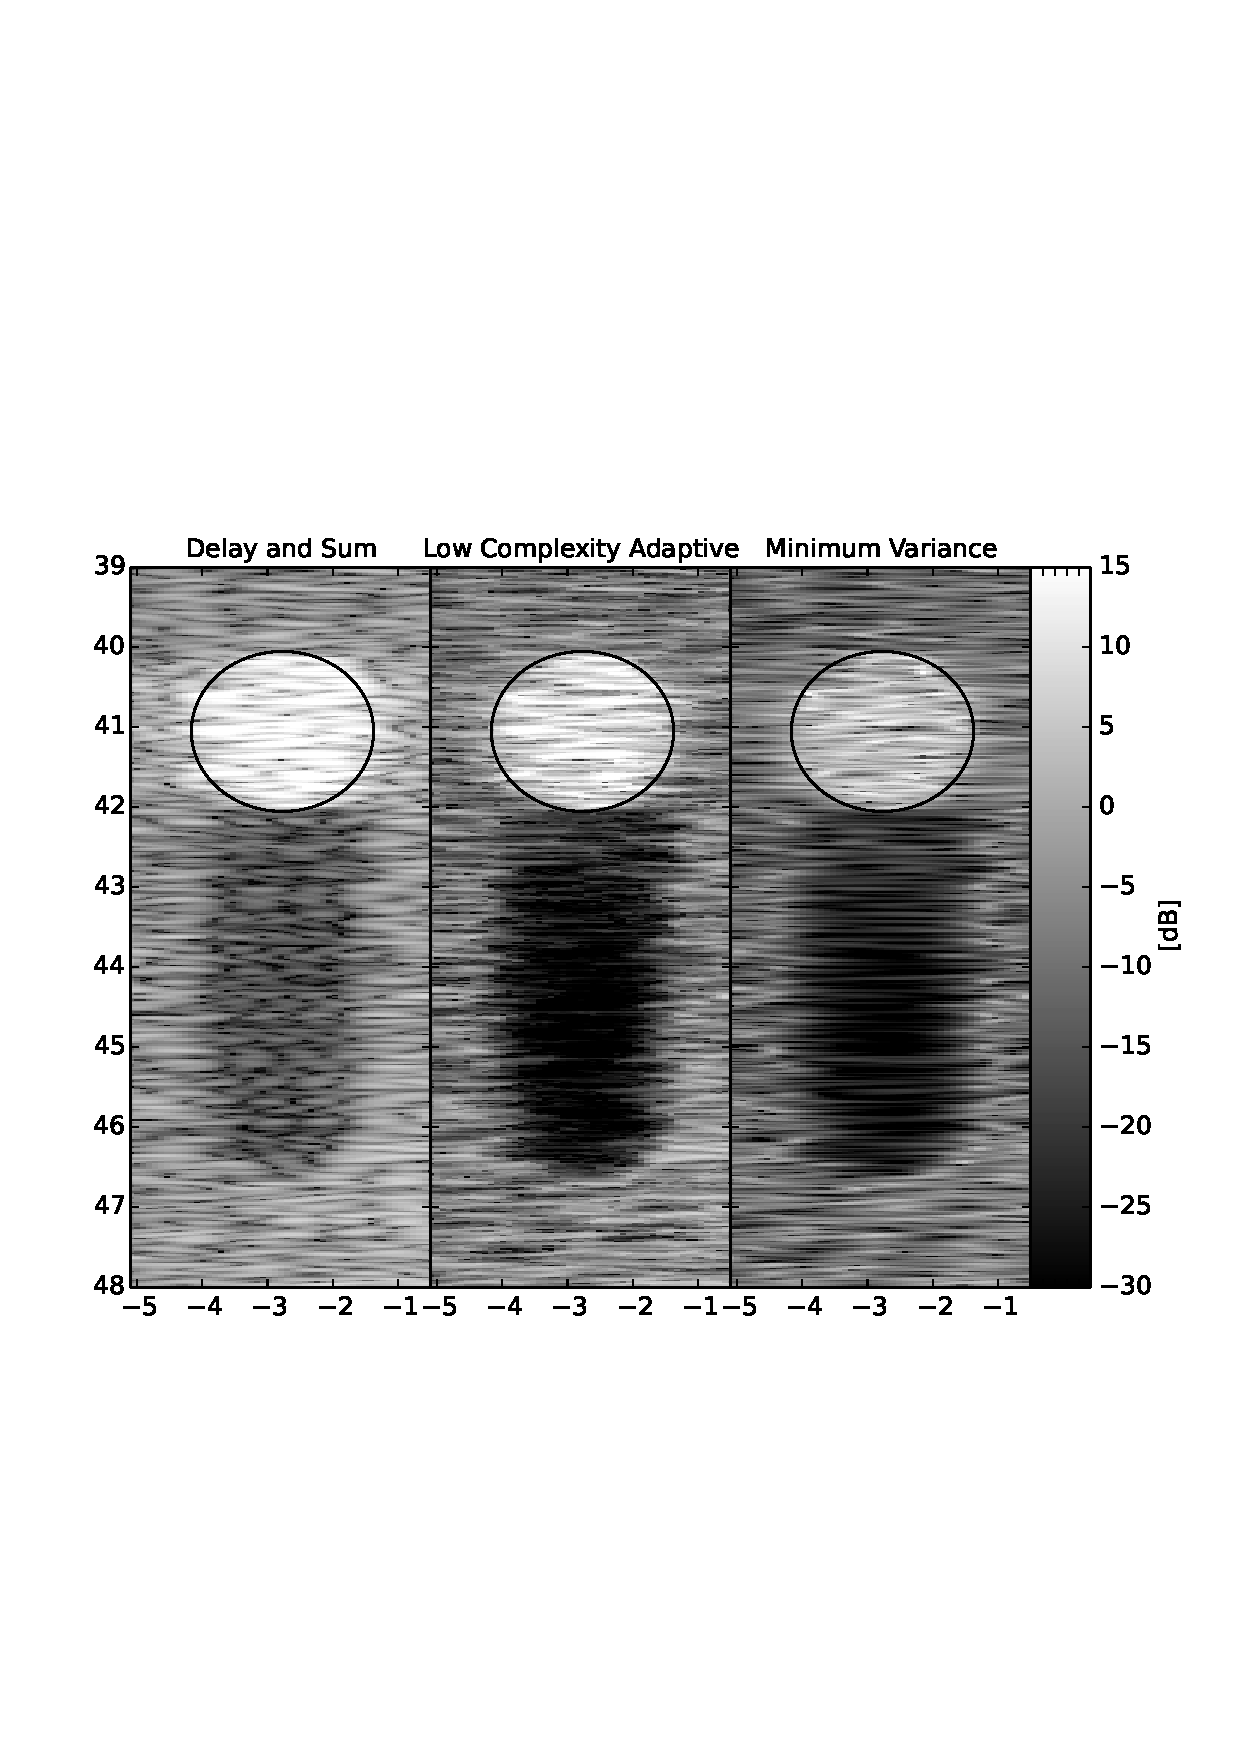
\includegraphics[width=0.49\linewidth]{gfx/4_mean_imgs.png}}\\
\subfloat[Windows ($\beta$)]{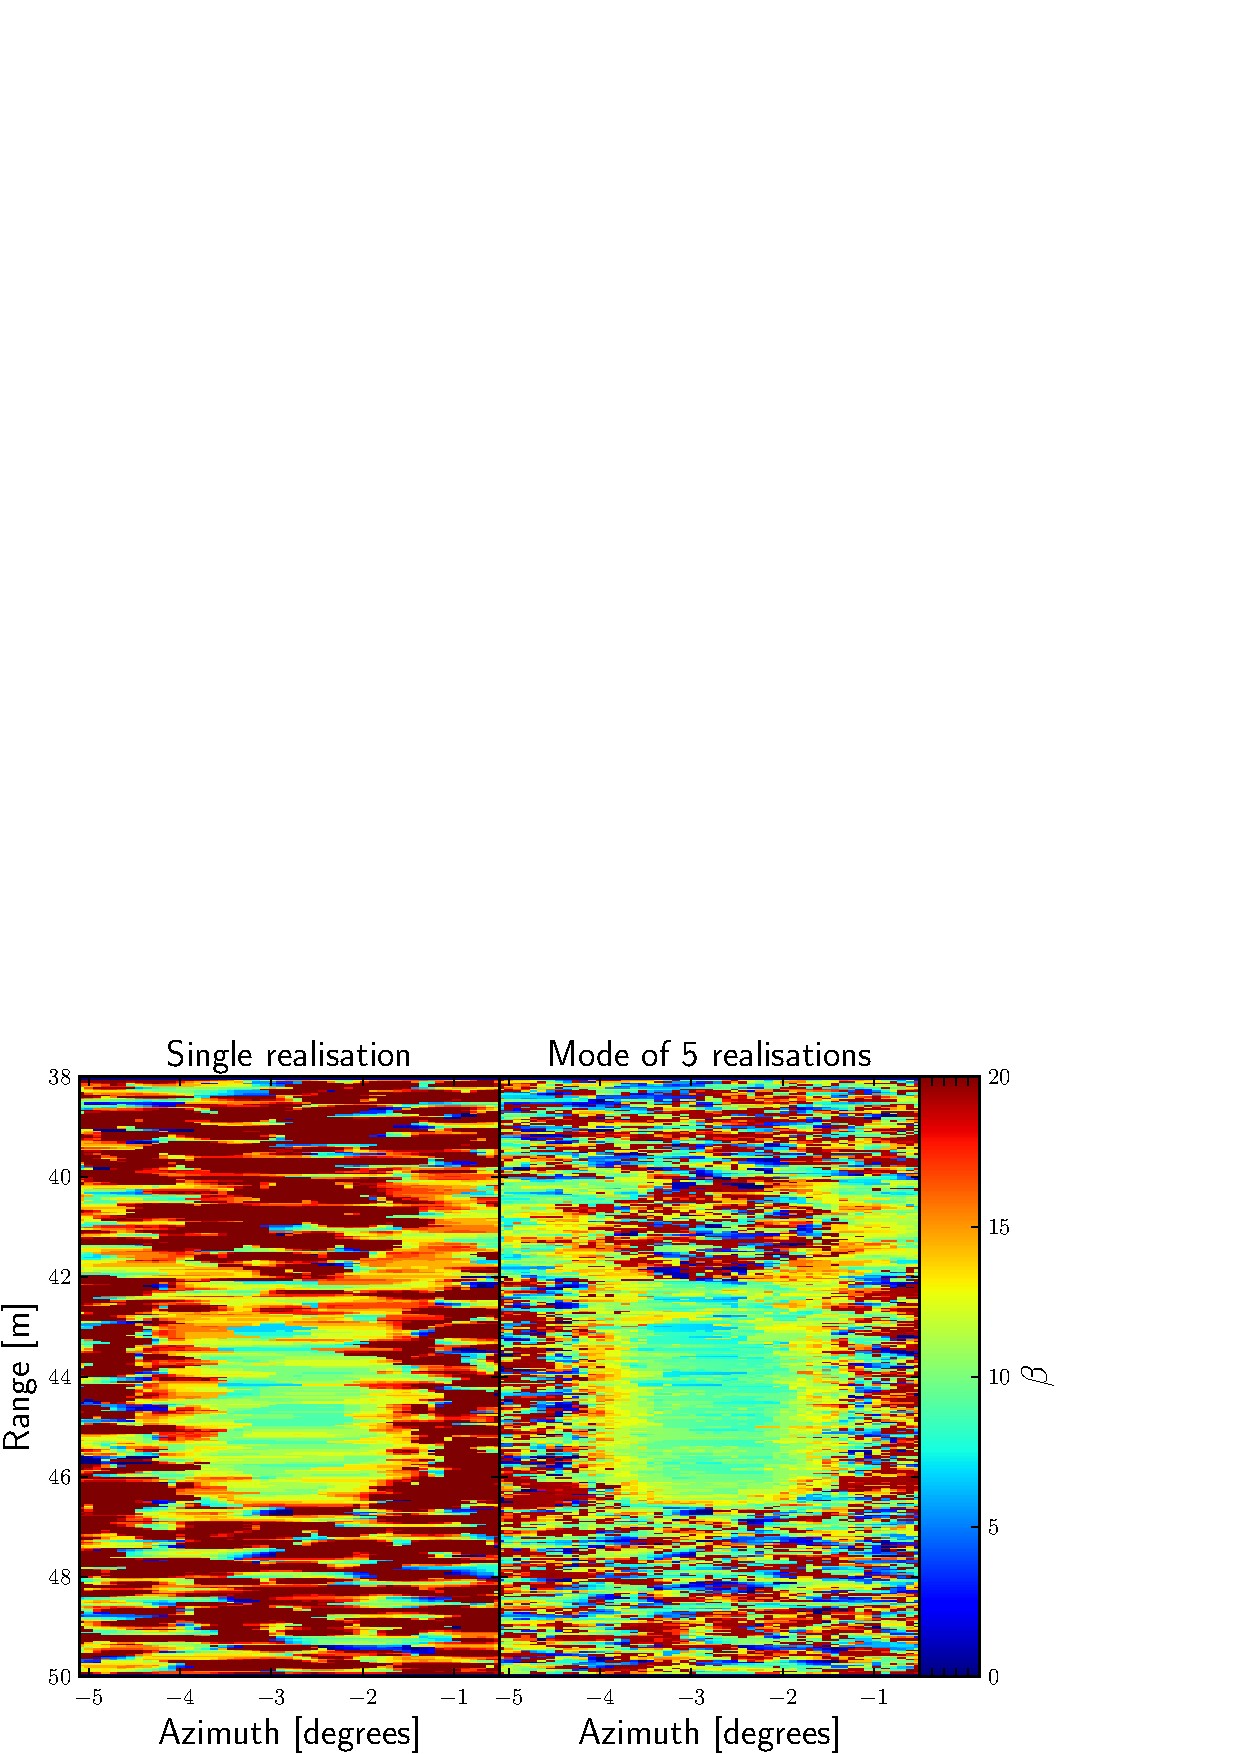
\includegraphics[width=0.49\linewidth]{gfx/4_windows_beta.png}}\hfill
\subfloat[Windows ($\phi$)]{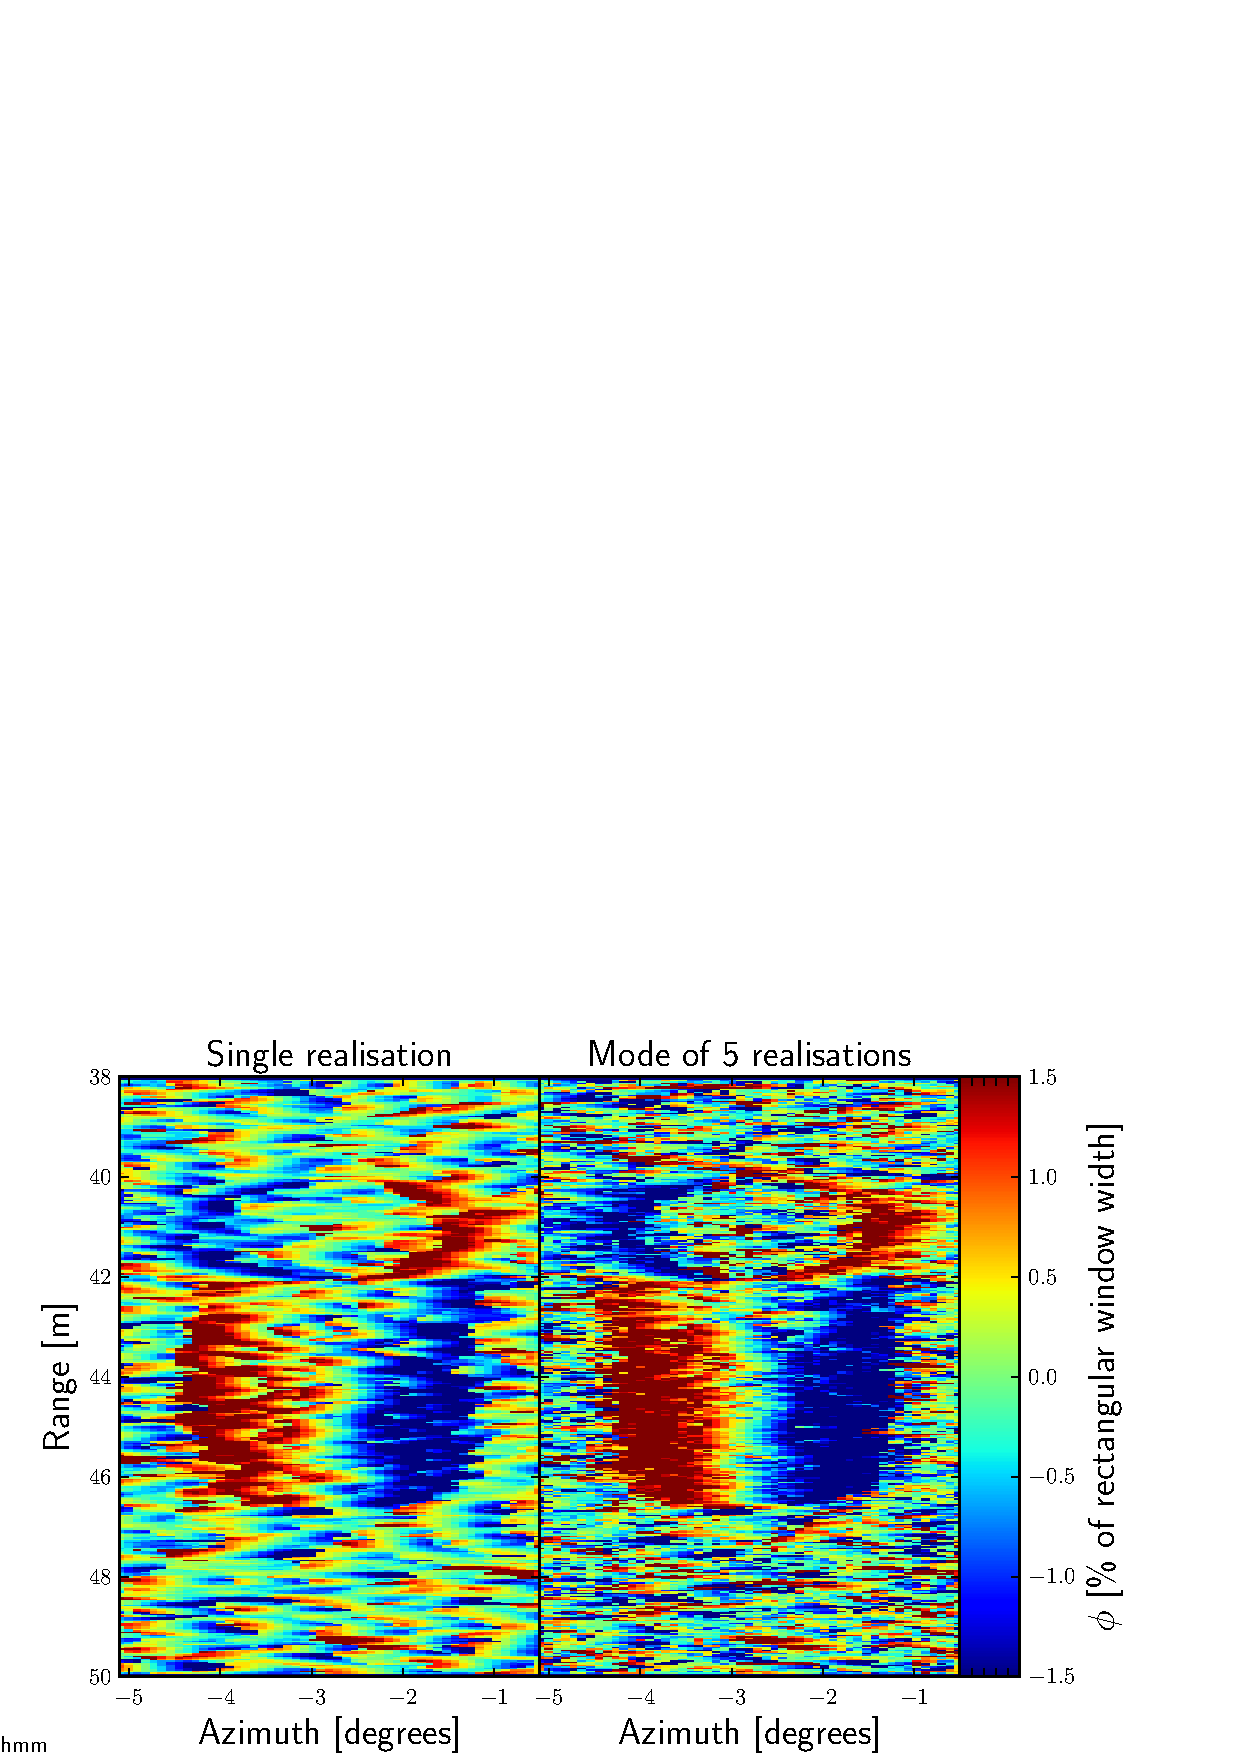
\includegraphics[width=0.48\linewidth]{gfx/4_windows_phi.png}}\\
\subfloat[Capon win. resp. through shadow]{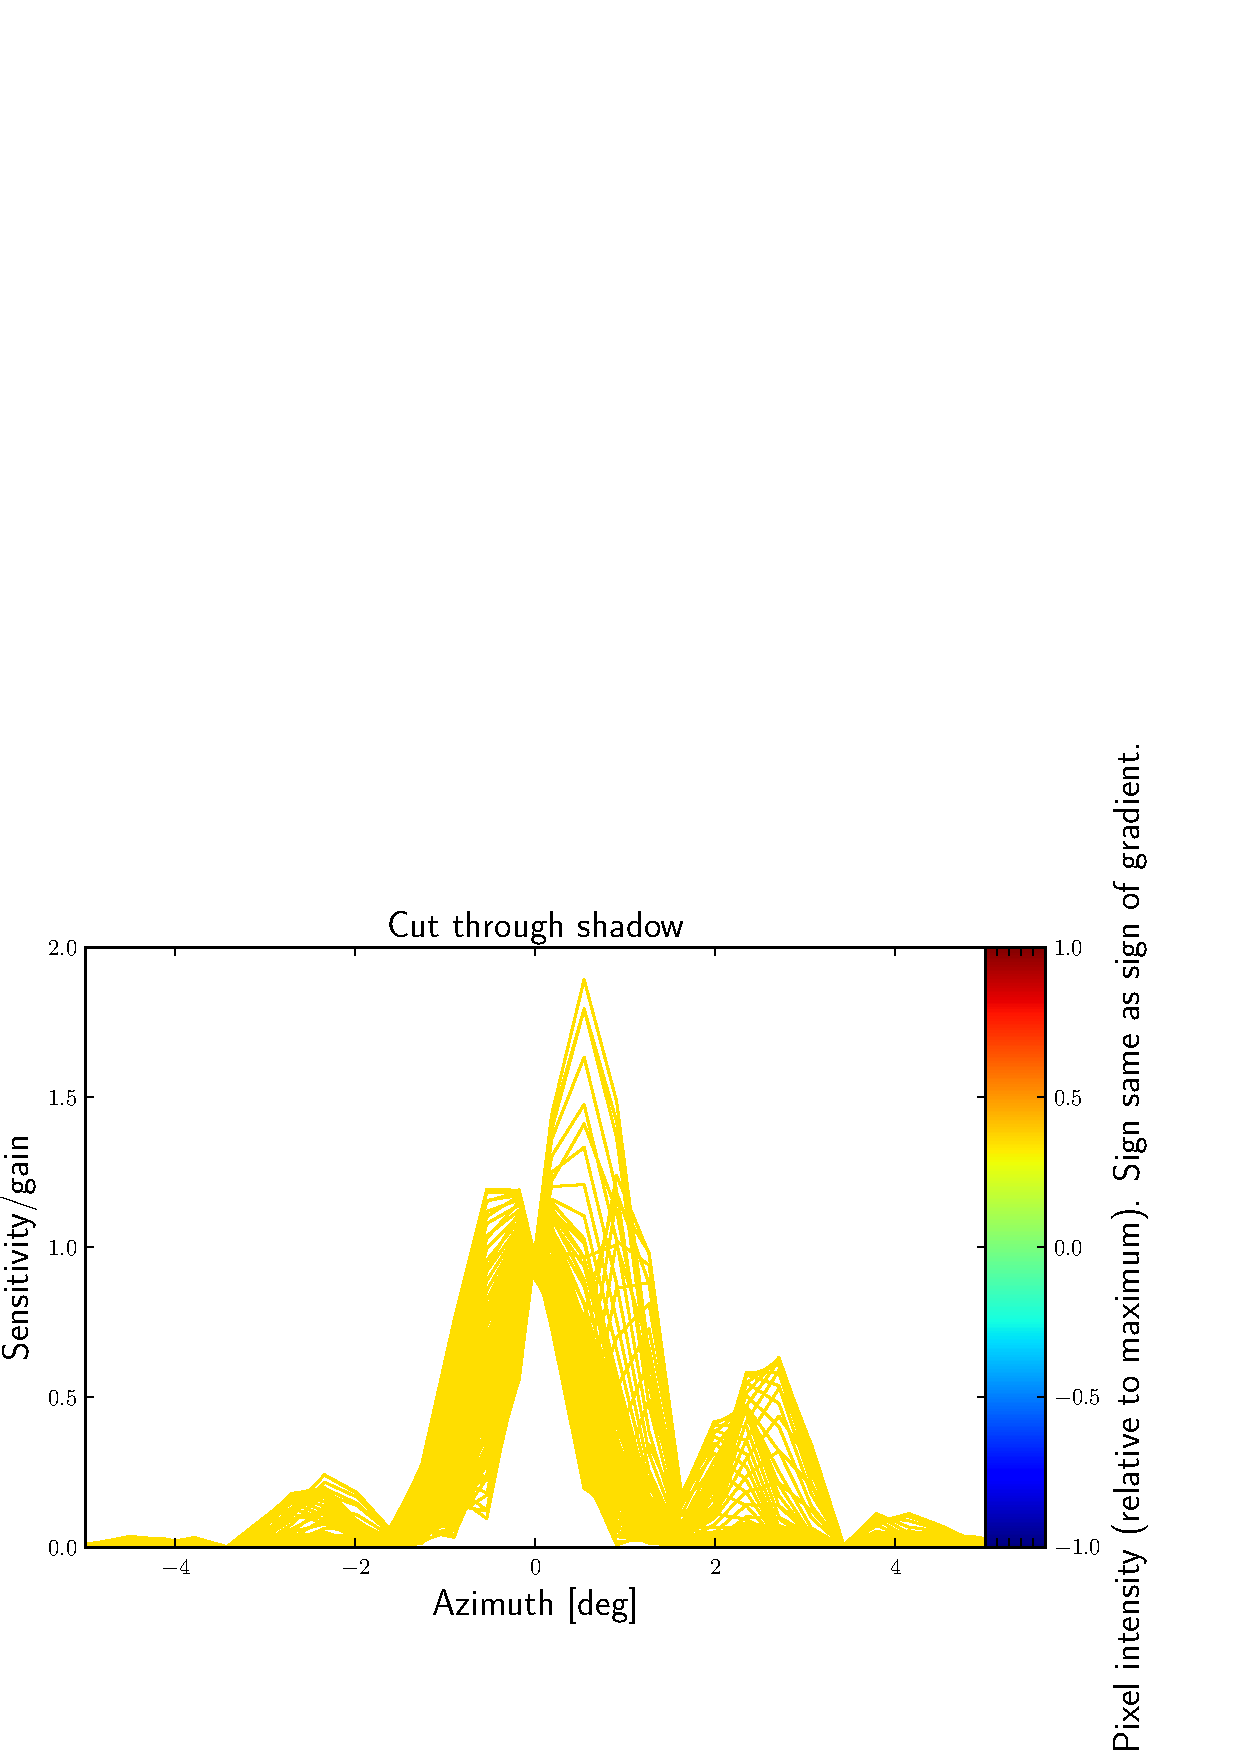
\includegraphics[width=0.49\linewidth]{gfx/4_win_resp_cut_shadow.png}}\hfill
\subfloat[Capon win. resp. through highlight]{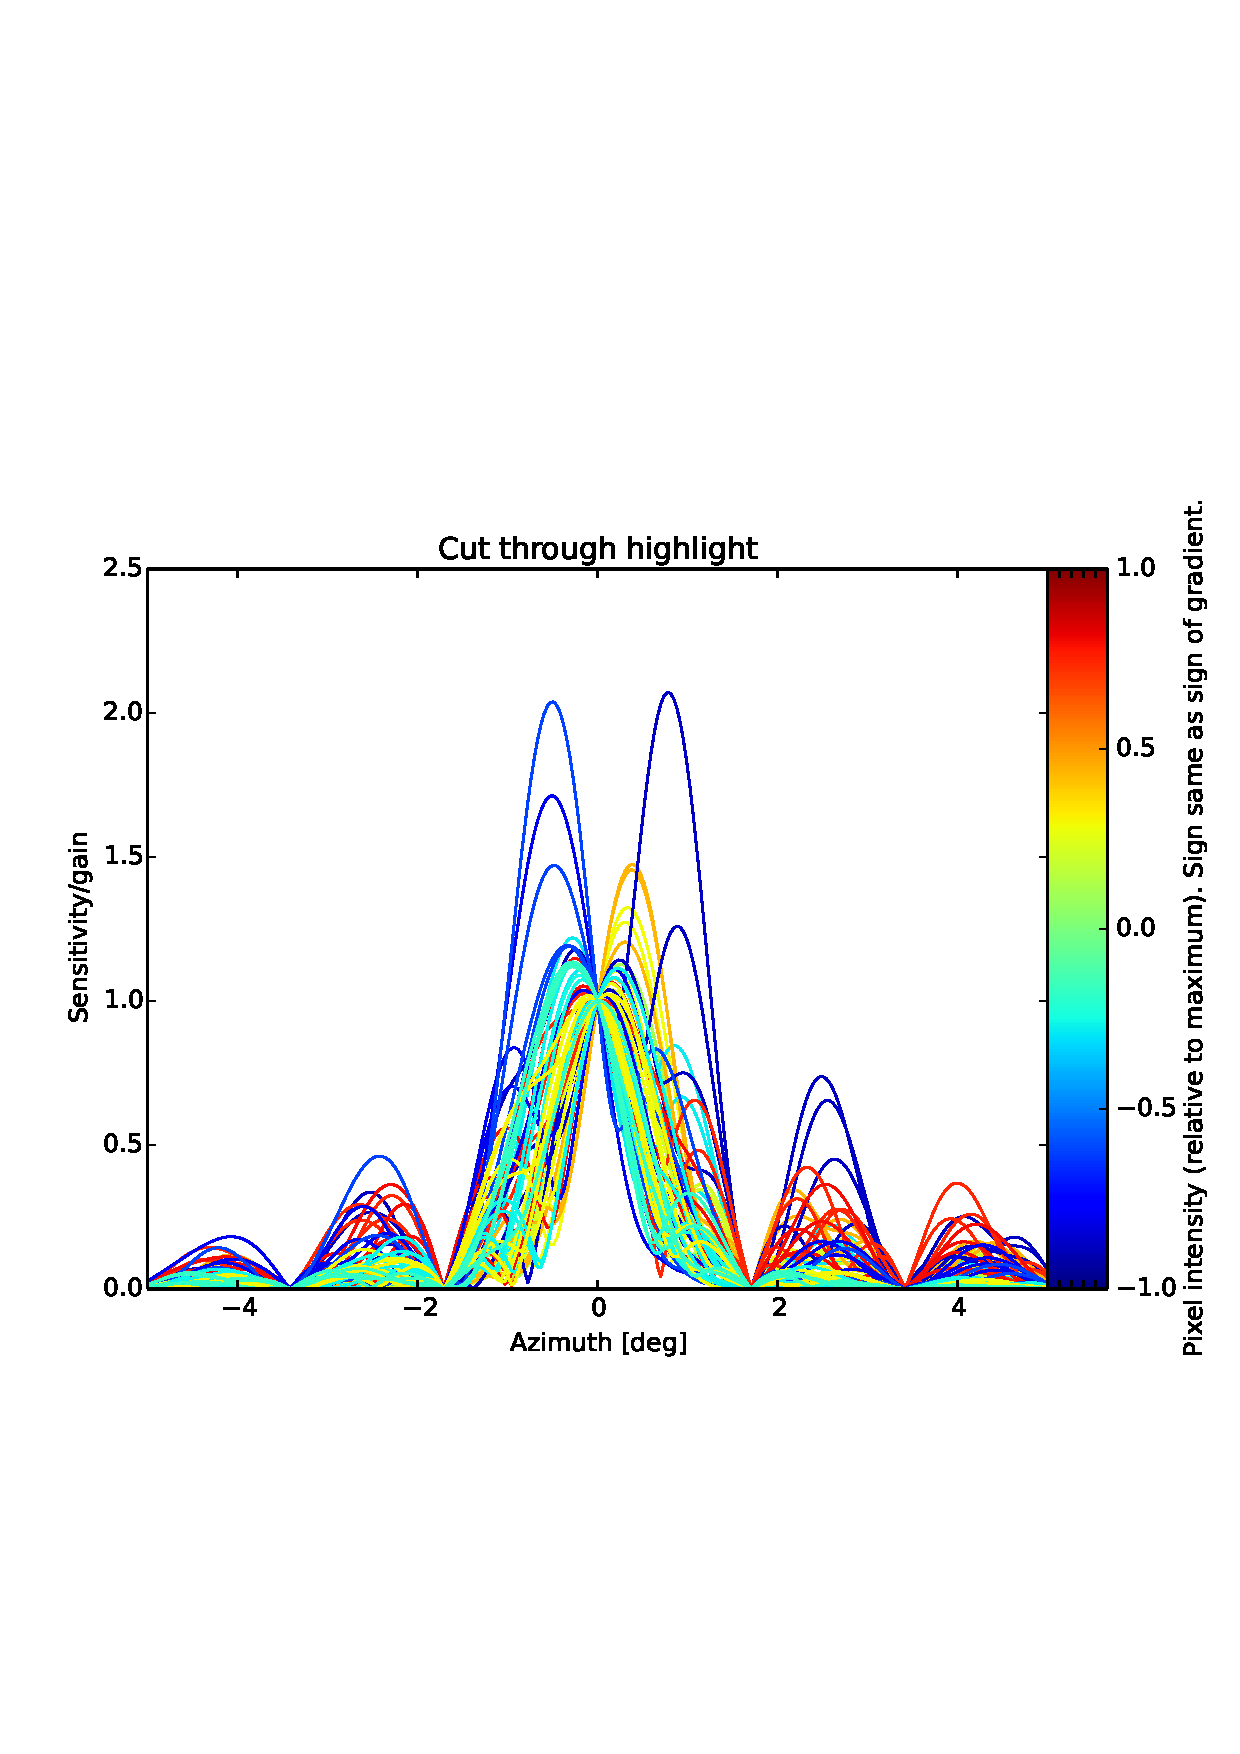
\includegraphics[width=0.49\linewidth]{gfx/4_win_resp_cut_highlight.png}}\\
\end{narrow}
\end{figure*}
\newpage
\begin{figure*}[!t]
\begin{narrow}{-1.2cm}{-1.2cm}\centering\vspace{-1.0cm}
\textbf{5. Capon: Tuning subarray.}\\
\begin{tabular}[c]{l l l l}
\bf General & M = 32                            & $\Delta r = \frac{c}{2B}$ = 2.5 cm & $\frac{640\,\text{pixels}] / 12\,\text{m}}{\Delta r} = \frac{4}{3}$ \\
\bf LCA     & $\beta \in [0,10]$ (9 values) & $\phi \in [-1.07,1.07]$ deg (9 values) & Navg = 3 \\
\bf Capon   & $\Delta$ = 0.01                 & L = 16                           & Navg = 3 \\
\end{tabular}
\subfloat[LCA Window Response]{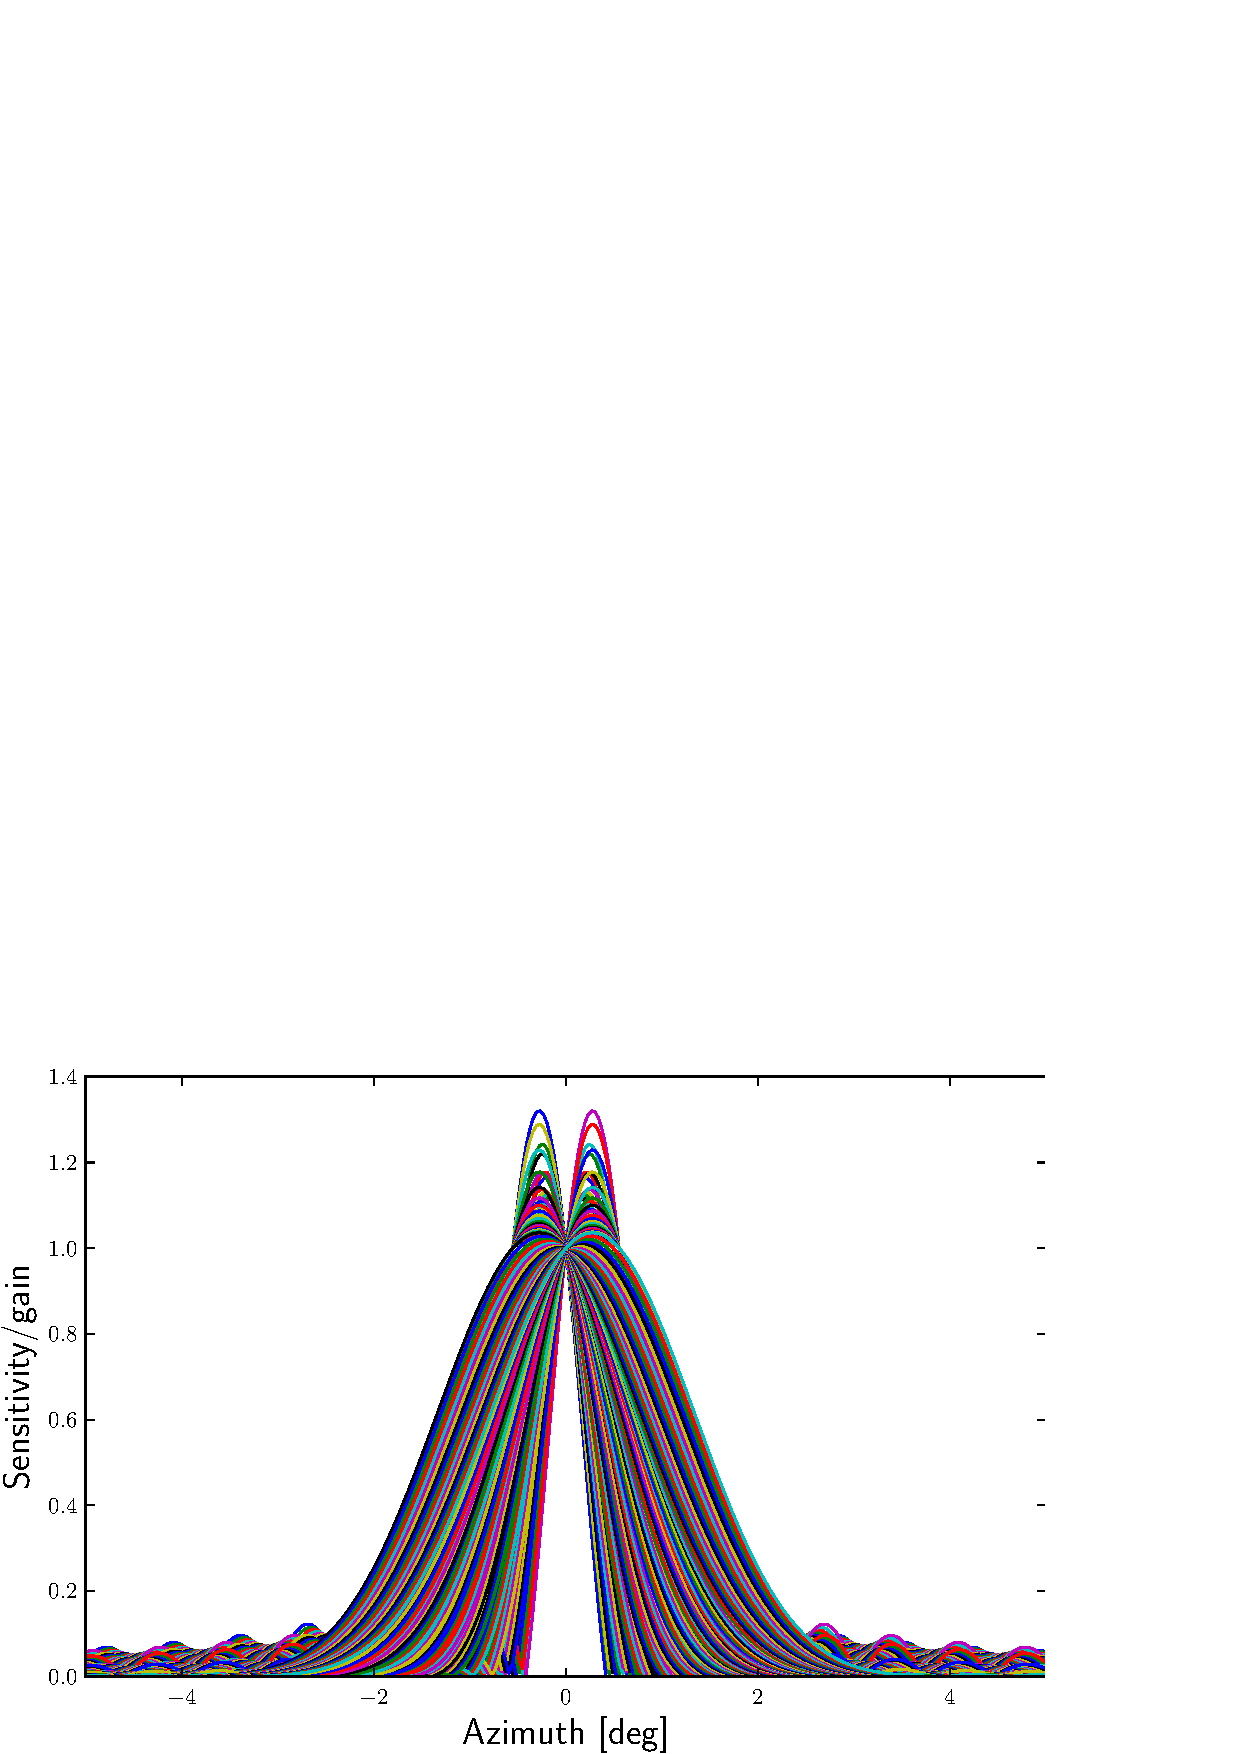
\includegraphics[width=0.49\linewidth]{gfx/5_window_response.png}}\hfill
\subfloat[Mean images]{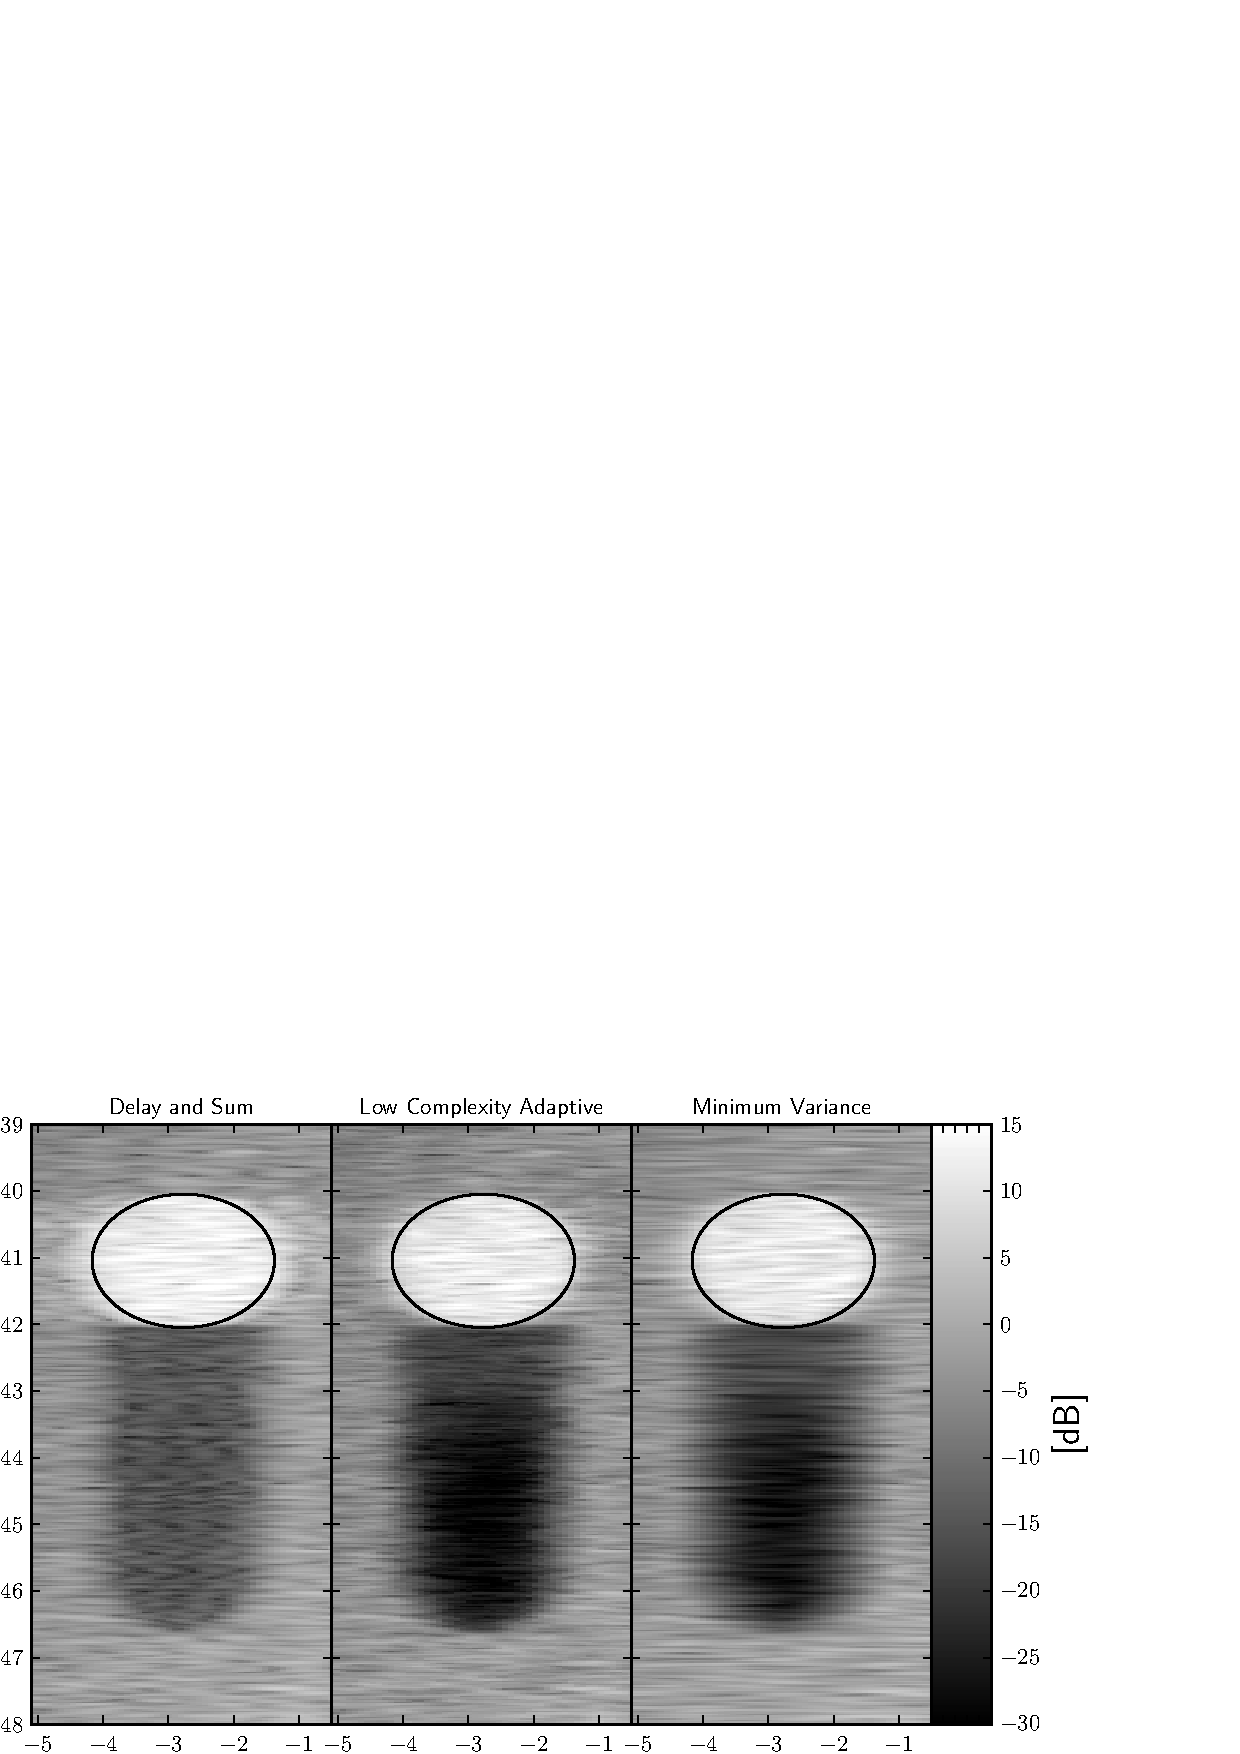
\includegraphics[width=0.49\linewidth]{gfx/5_mean_imgs.png}}\\
\subfloat[Windows ($\beta$)]{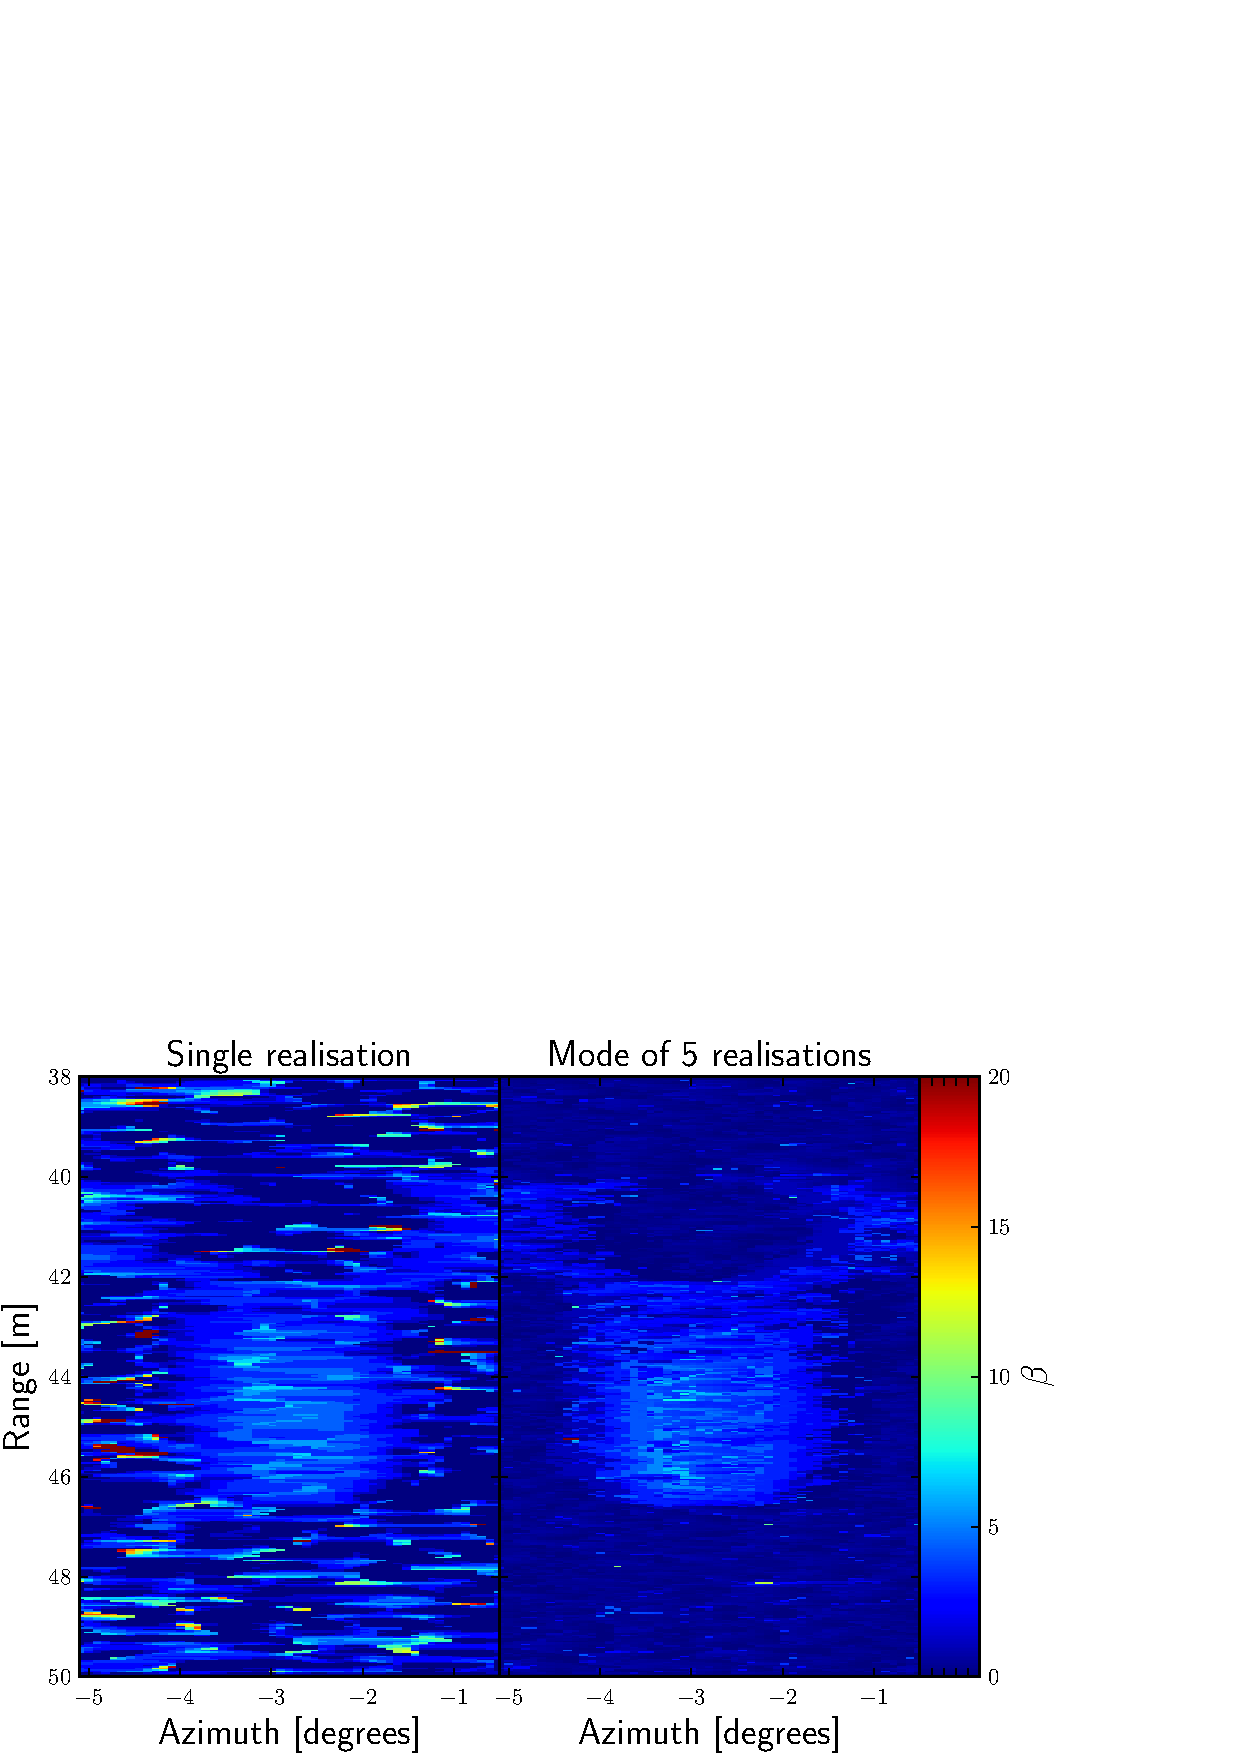
\includegraphics[width=0.49\linewidth]{gfx/5_windows_beta.png}}\hfill
\subfloat[Windows ($\phi$)]{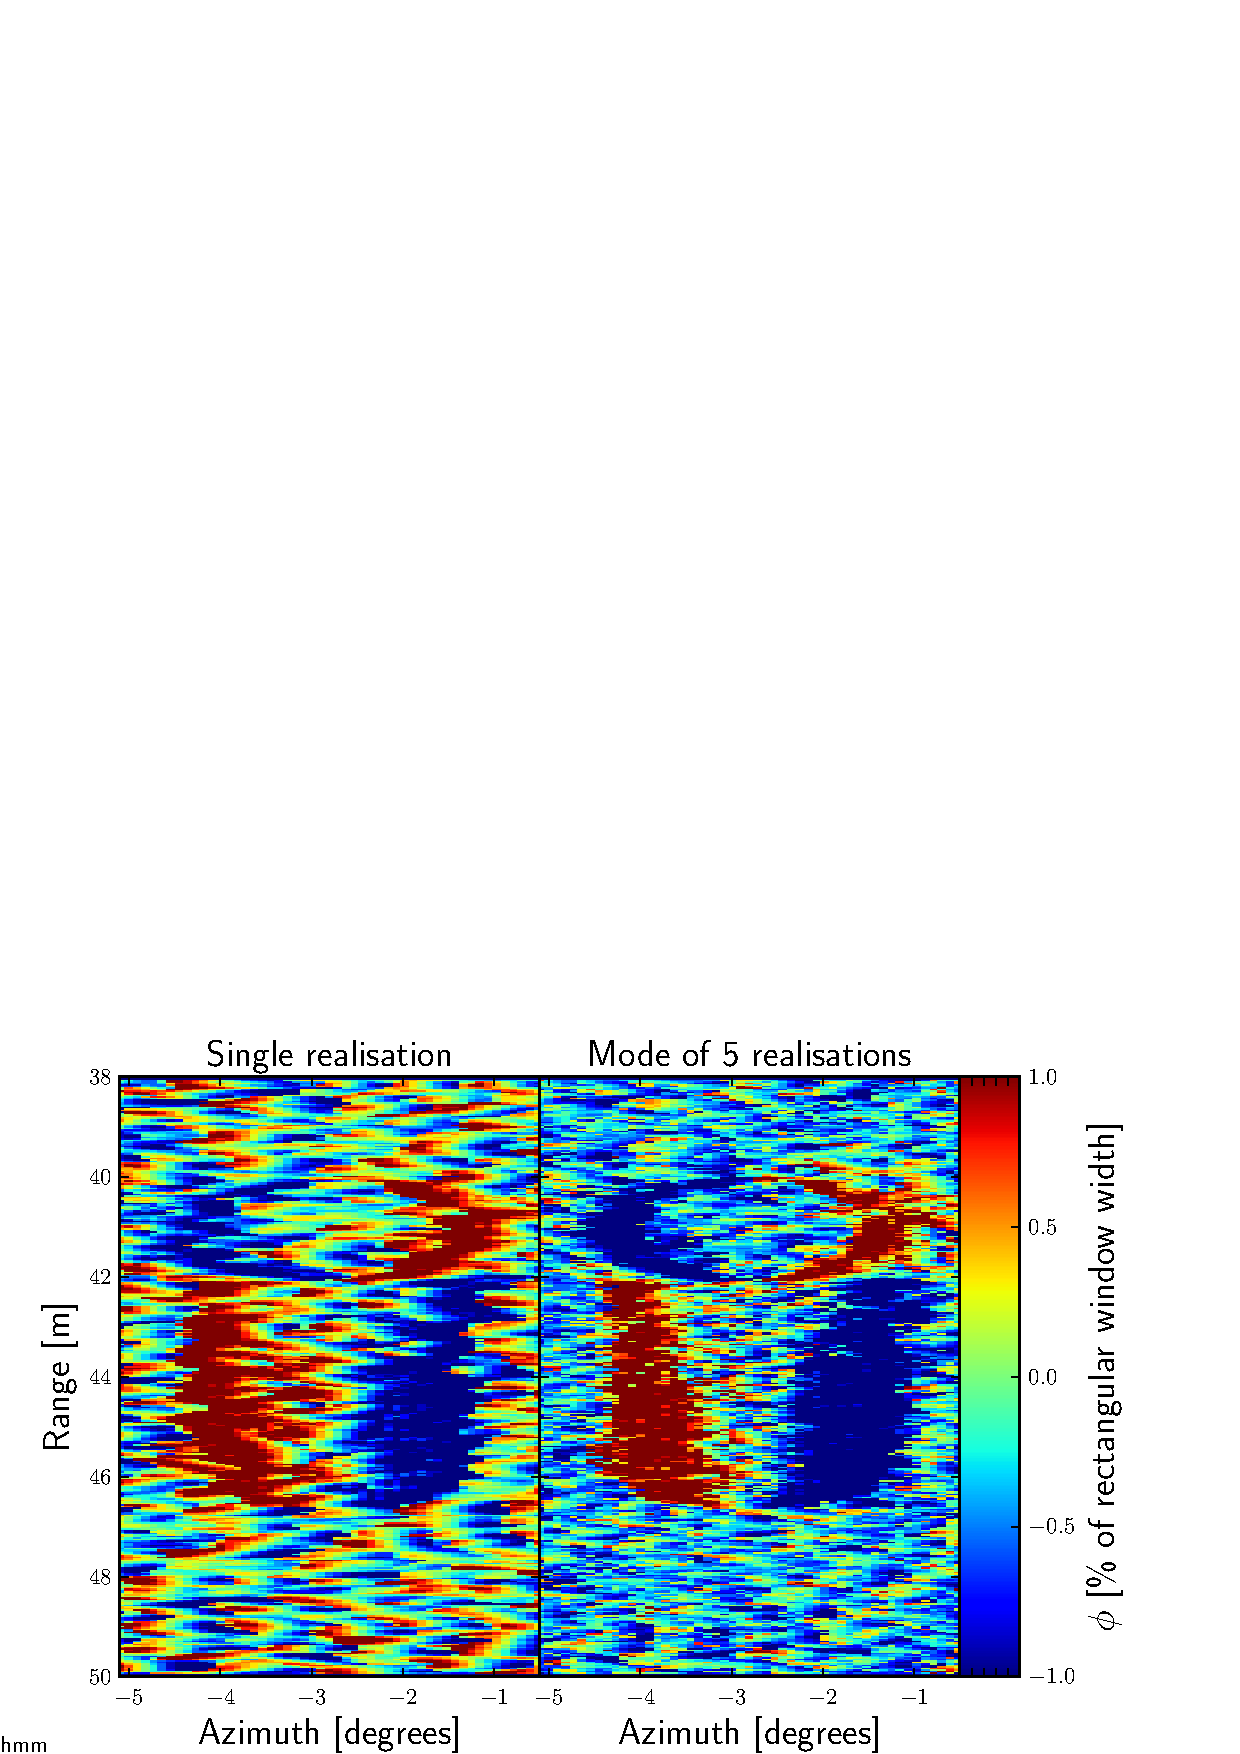
\includegraphics[width=0.48\linewidth]{gfx/5_windows_phi.png}}\\
\subfloat[Capon win. resp. through shadow]{\includegraphics[width=0.49\linewidth]{gfx/5_win_resp_cut_shadow.png}}\hfill
\subfloat[Capon win. resp. through highlight]{\includegraphics[width=0.49\linewidth]{gfx/5_win_resp_cut_highlight.png}}\\
\end{narrow}
\end{figure*}
\newpage
\begin{figure*}[!t]
\begin{narrow}{-1.2cm}{-1.2cm}\centering\vspace{-1.0cm}
\textbf{6. Capon: Tuning subarray.}\\
\begin{tabular}[c]{l l l l}
\bf General & M = 32                            & $\Delta r = \frac{c}{2B}$ = 2.5 cm & $\frac{640\,\text{pixels}] / 12\,\text{m}}{\Delta r} = \frac{4}{3}$ \\
\bf LCA     & $\beta \in [0,10]$ (9 values) & $\phi \in [-1.07,1.07]$ deg (9 values) & Navg = 3 \\
\bf Capon   & $\Delta$ = 0.01                 & L = 12                           & Navg = 3 \\
\end{tabular}
\subfloat[LCA Window Response]{\includegraphics[width=0.49\linewidth]{gfx/6_window_response.png}}\hfill
\subfloat[Mean images]{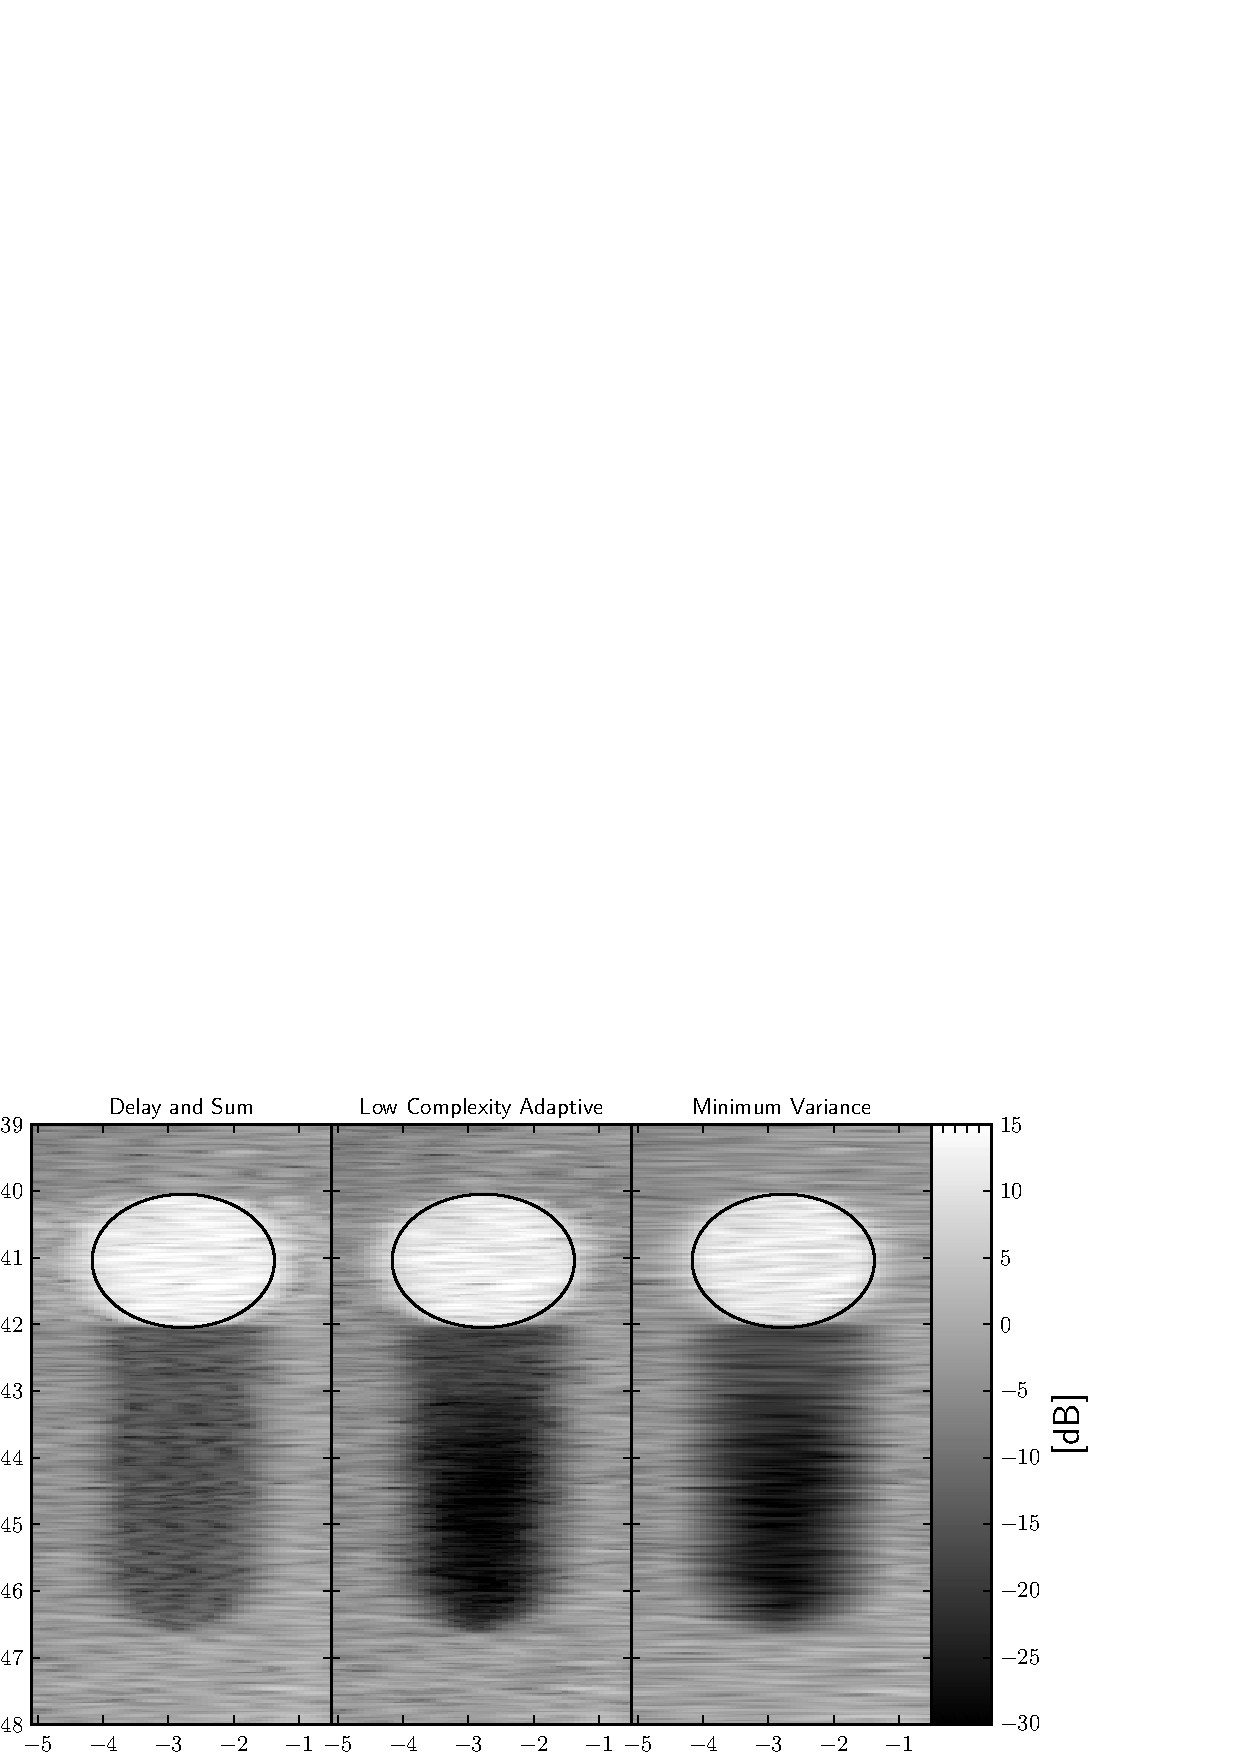
\includegraphics[width=0.49\linewidth]{gfx/6_mean_imgs.png}}\\
\subfloat[Windows ($\beta$)]{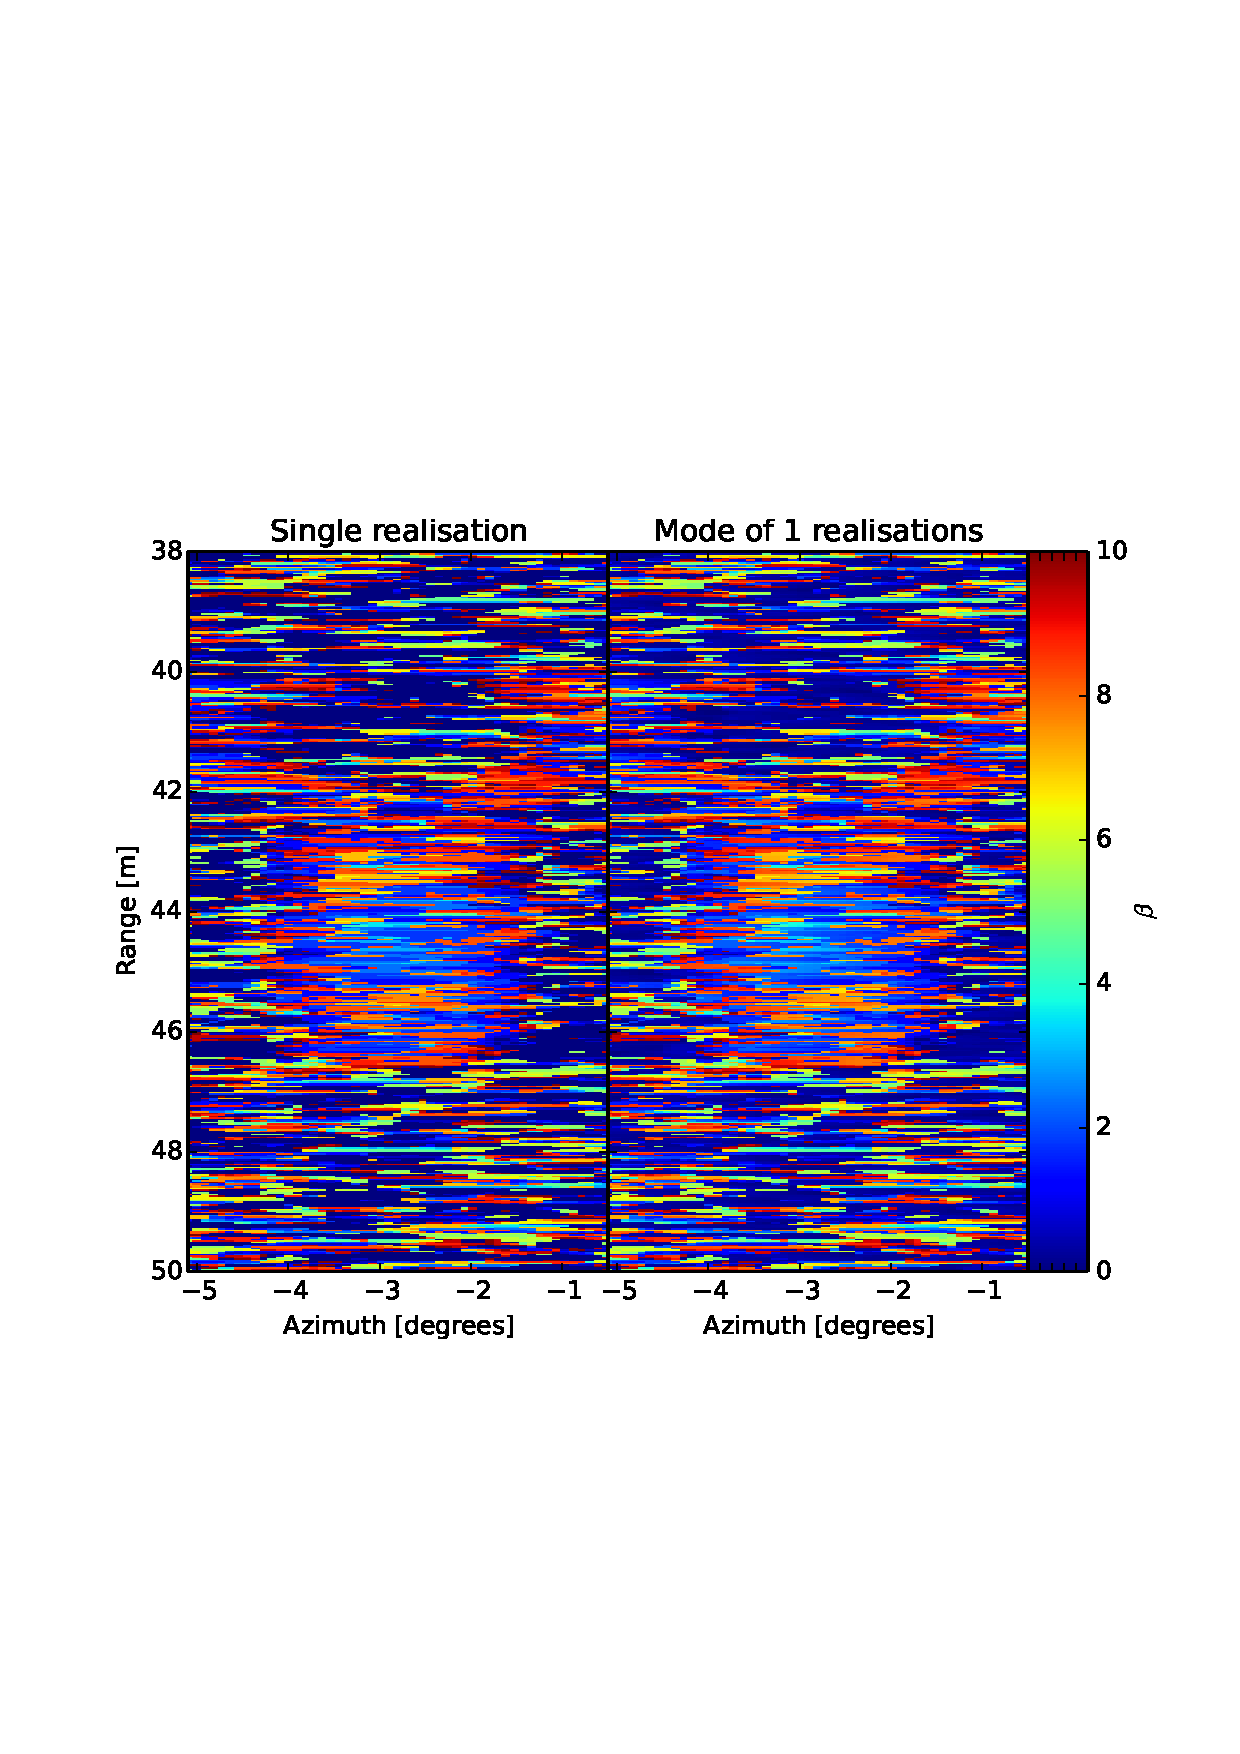
\includegraphics[width=0.49\linewidth]{gfx/6_windows_beta.png}}\hfill
\subfloat[Windows ($\phi$)]{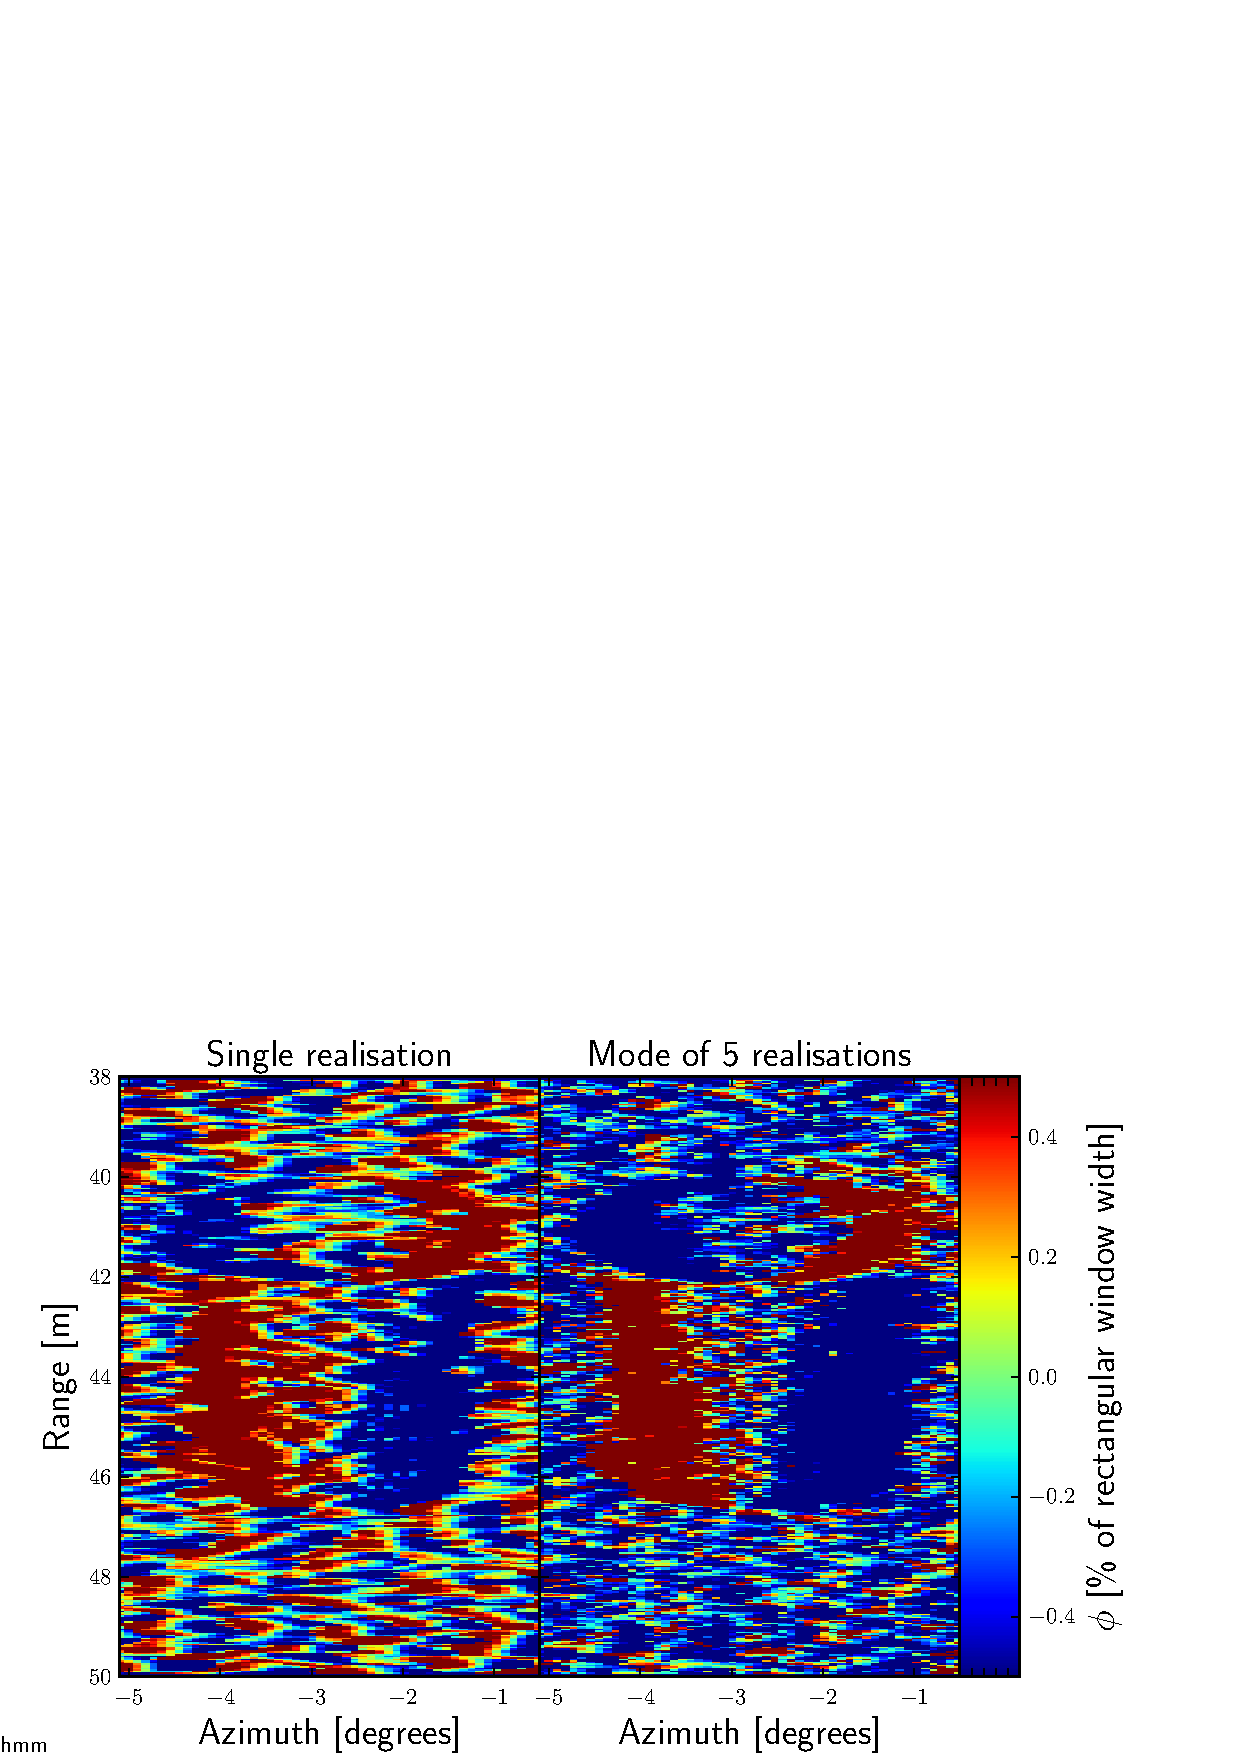
\includegraphics[width=0.48\linewidth]{gfx/6_windows_phi.png}}\\
\subfloat[Capon win. resp. through shadow]{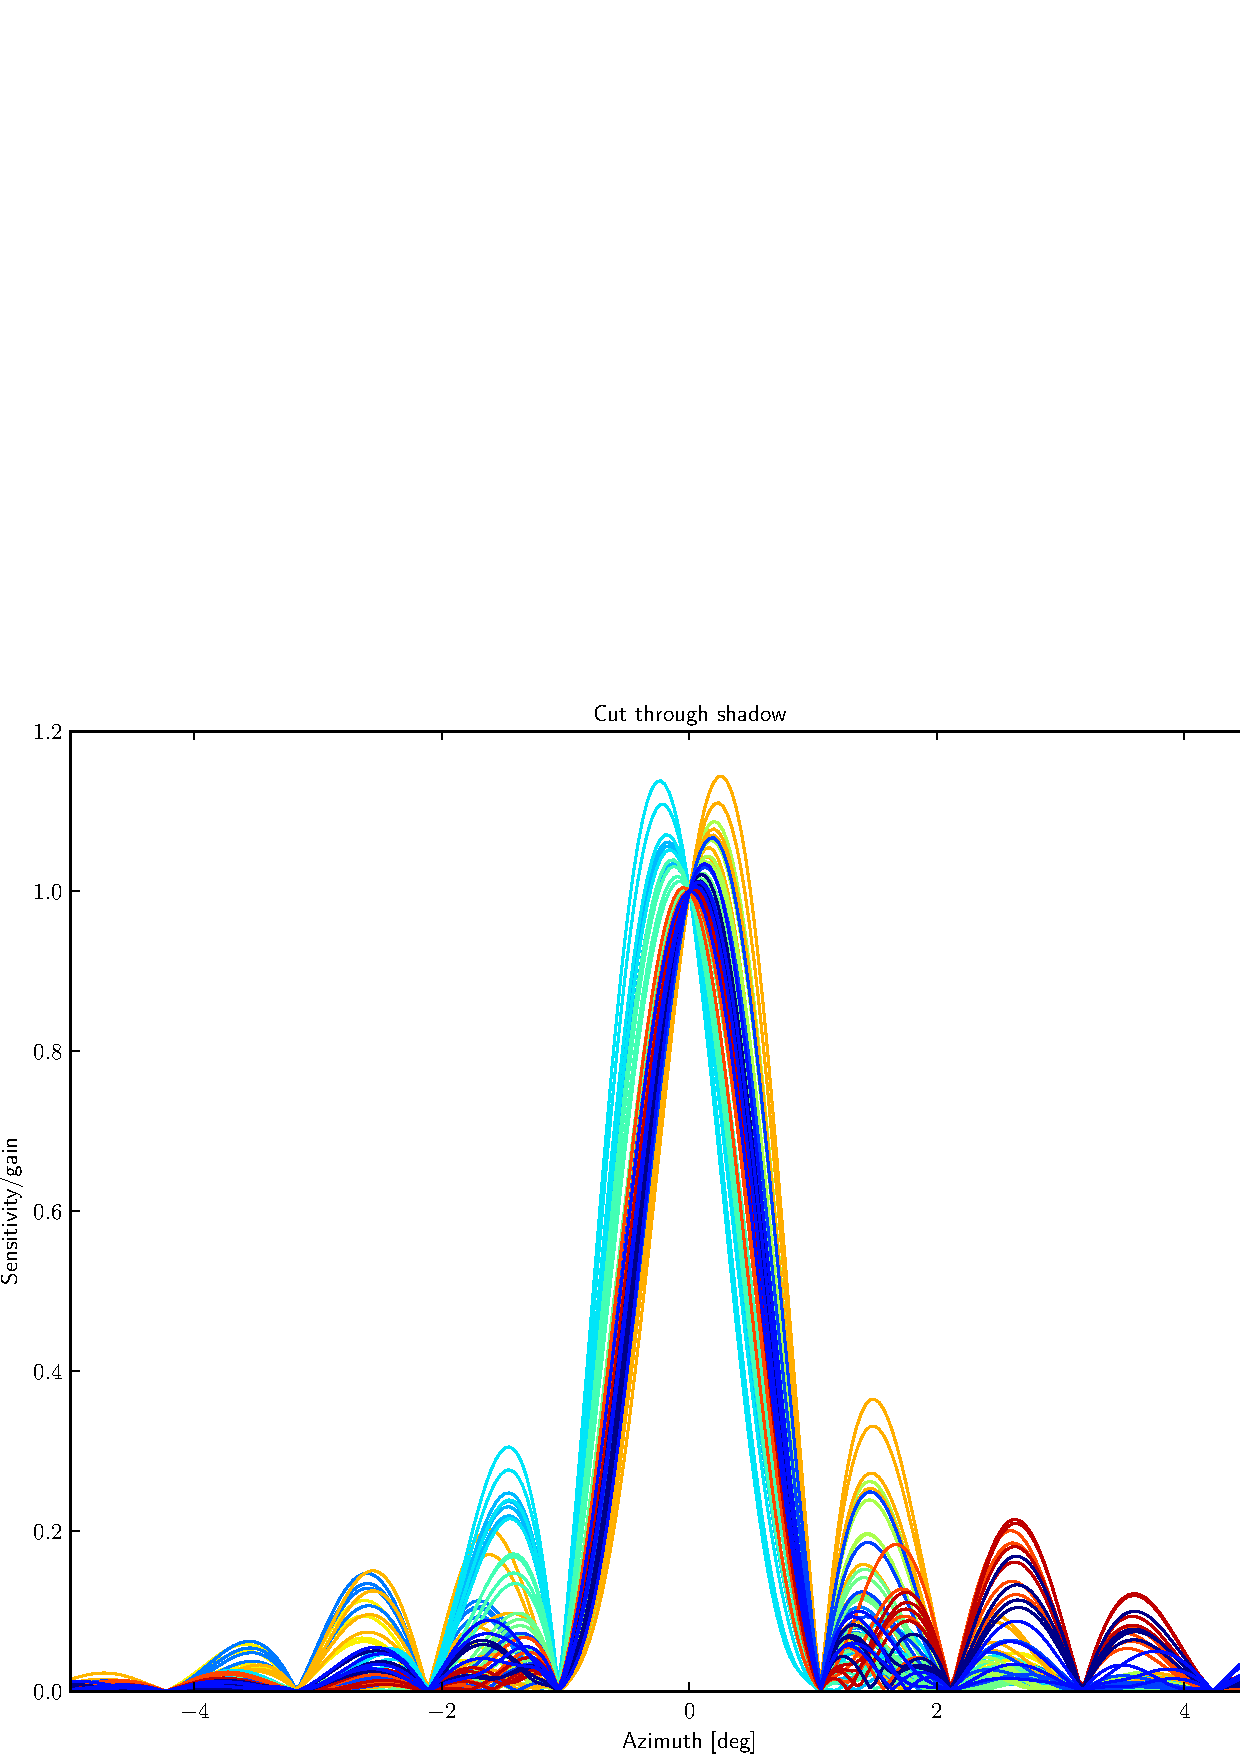
\includegraphics[width=0.49\linewidth]{gfx/6_win_resp_cut_shadow.png}}\hfill
\subfloat[Capon win. resp. through highlight]{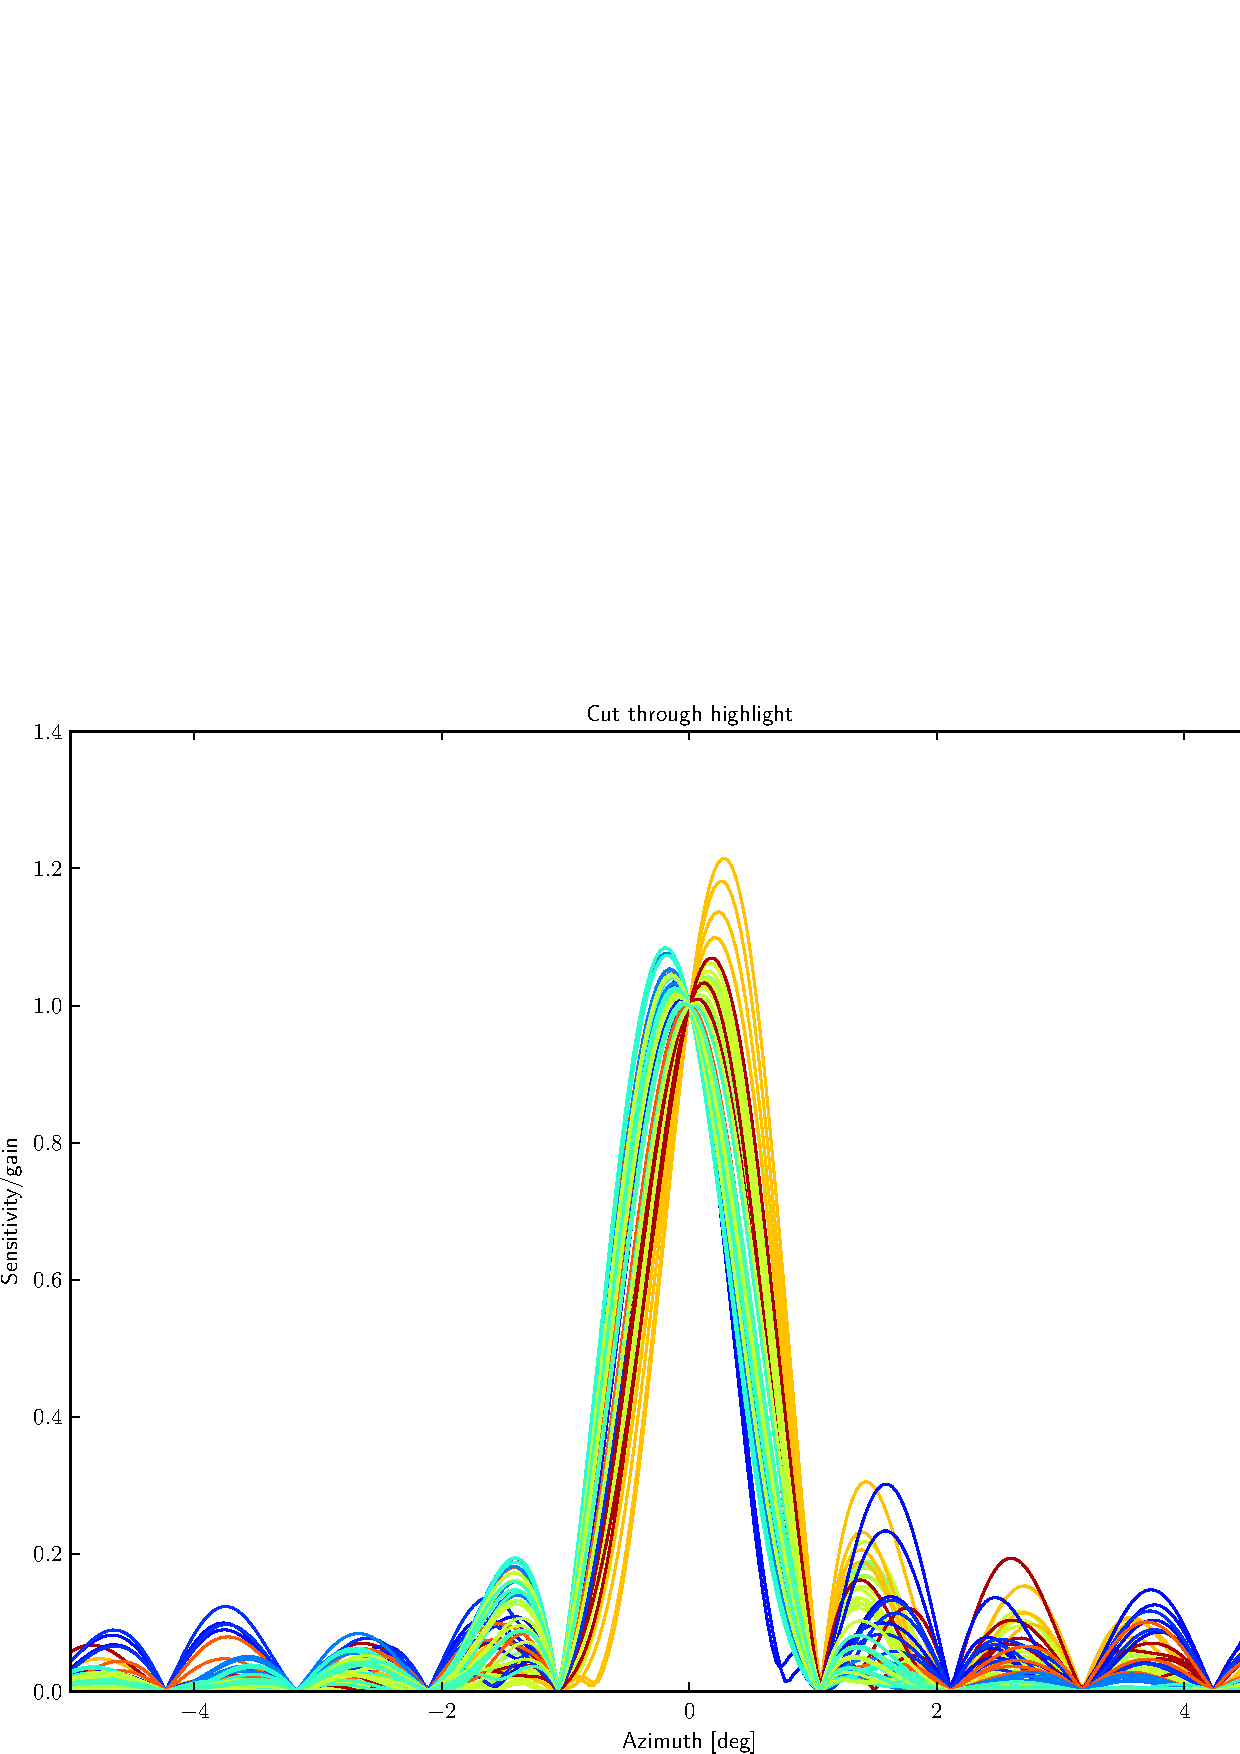
\includegraphics[width=0.49\linewidth]{gfx/6_win_resp_cut_highlight.png}}\\
\end{narrow}
\end{figure*}
\newpage
\begin{figure*}[!t]
\begin{narrow}{-1.2cm}{-1.2cm}\centering\vspace{-1.0cm}
\textbf{7. Capon: Tuning time averaging.}\\
\begin{tabular}[c]{l l l l}
\bf General & M = 32                            & $\Delta r = \frac{c}{2B}$ = 2.5 cm & $\frac{640\,\text{pixels}] / 12\,\text{m}}{\Delta r} = \frac{4}{3}$ \\
\bf LCA     & $\beta \in [0,10]$ (9 values) & $\phi \in [-1.07,1.07]$ deg (9 values) & Navg = 1 \\
\bf Capon   & $\Delta$ = 0.01                 & L = 16                           & Navg = 1 \\
\end{tabular}
\subfloat[LCA Window Response]{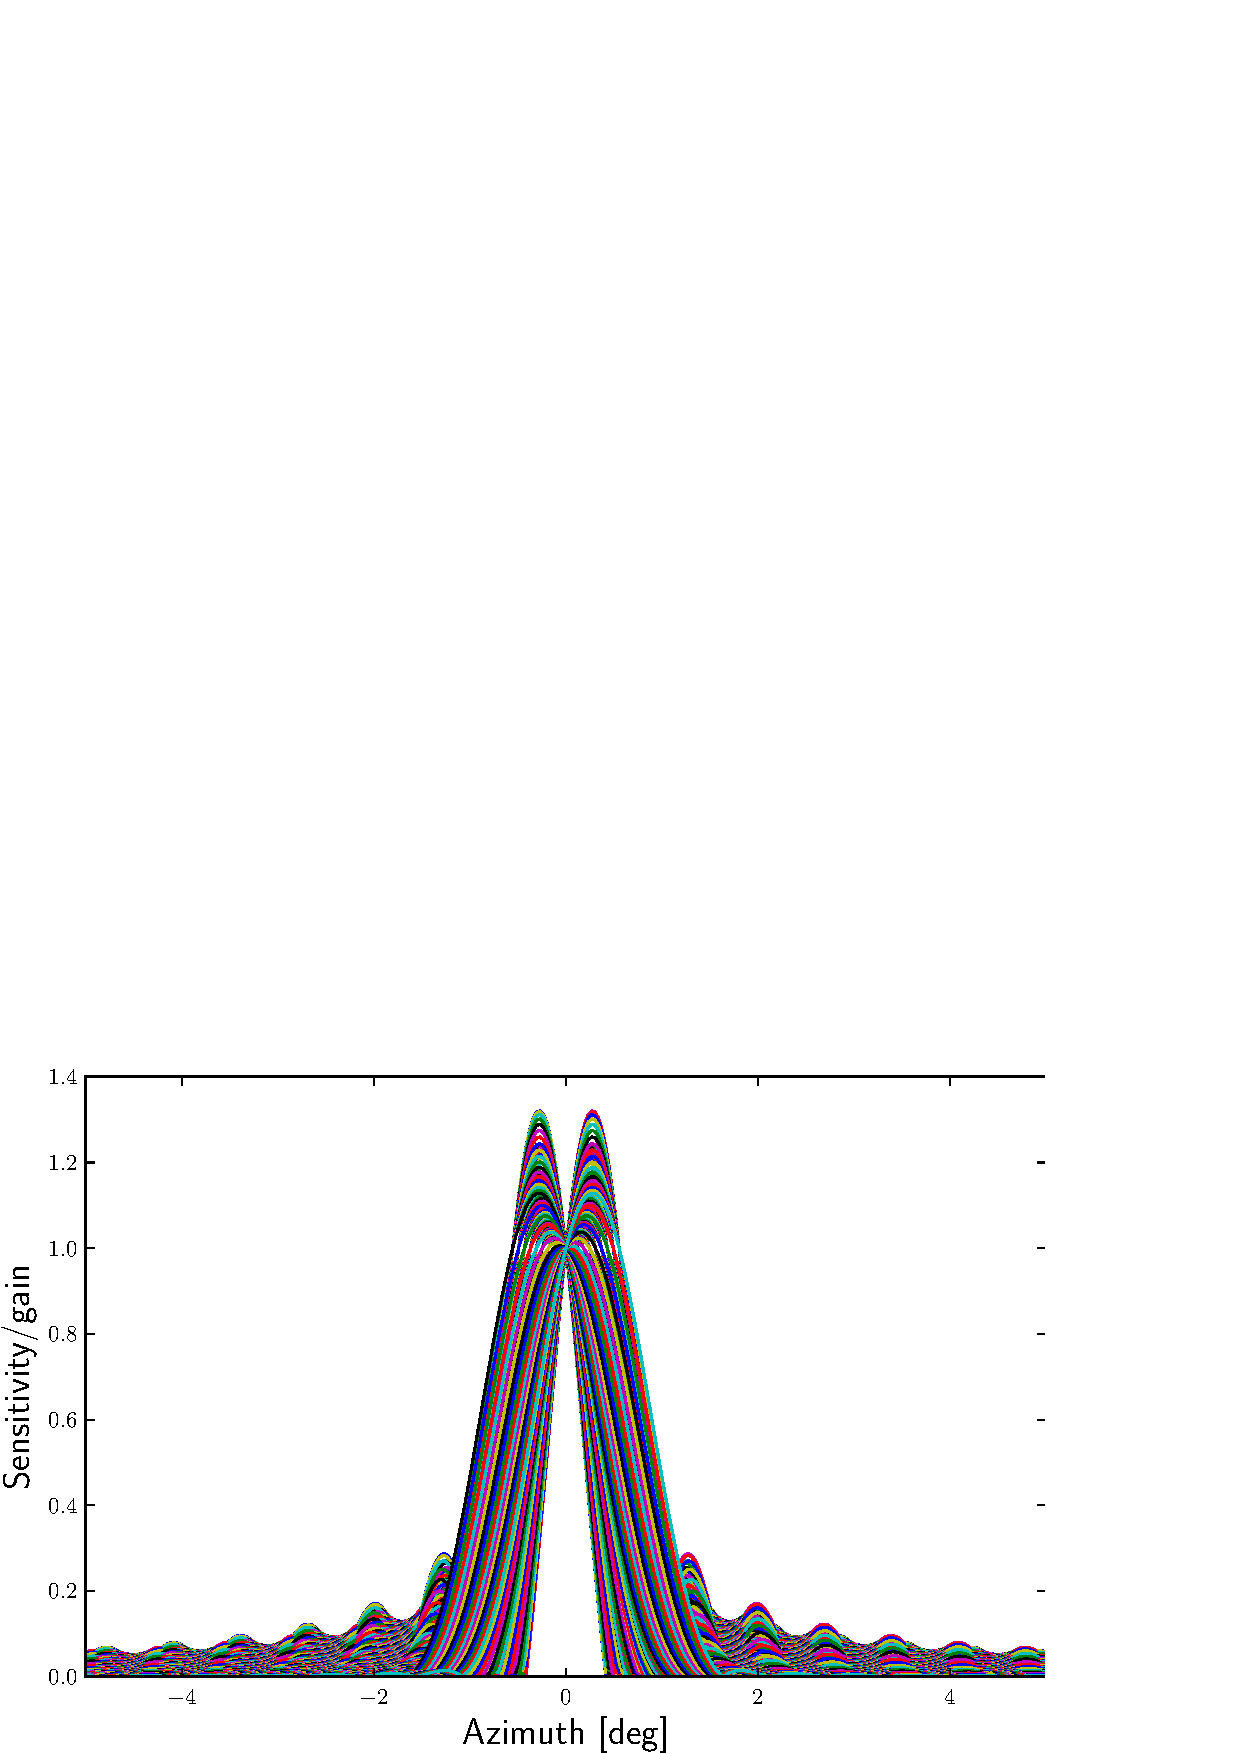
\includegraphics[width=0.49\linewidth]{gfx/7_window_response.png}}\hfill
\subfloat[Mean images]{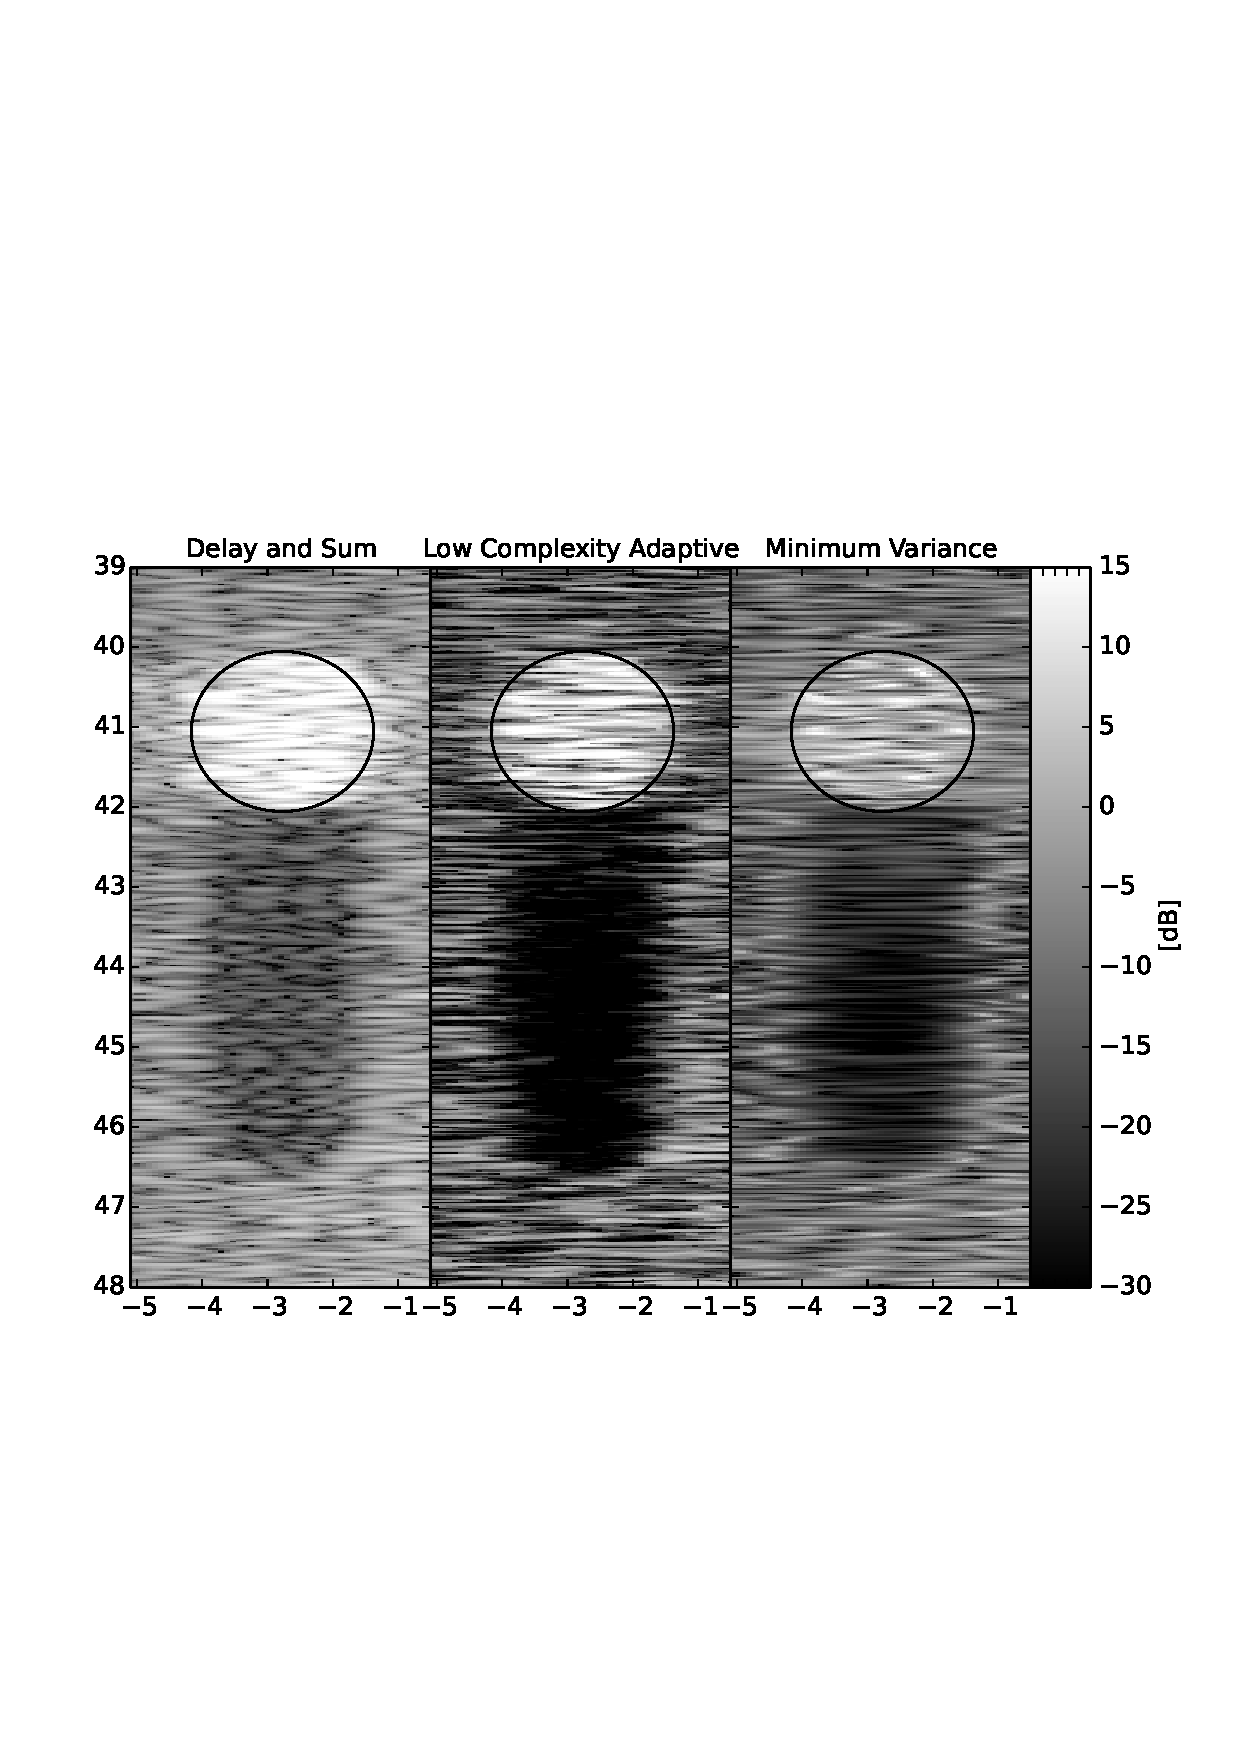
\includegraphics[width=0.49\linewidth]{gfx/7_mean_imgs.png}}\\
\subfloat[Windows ($\beta$)]{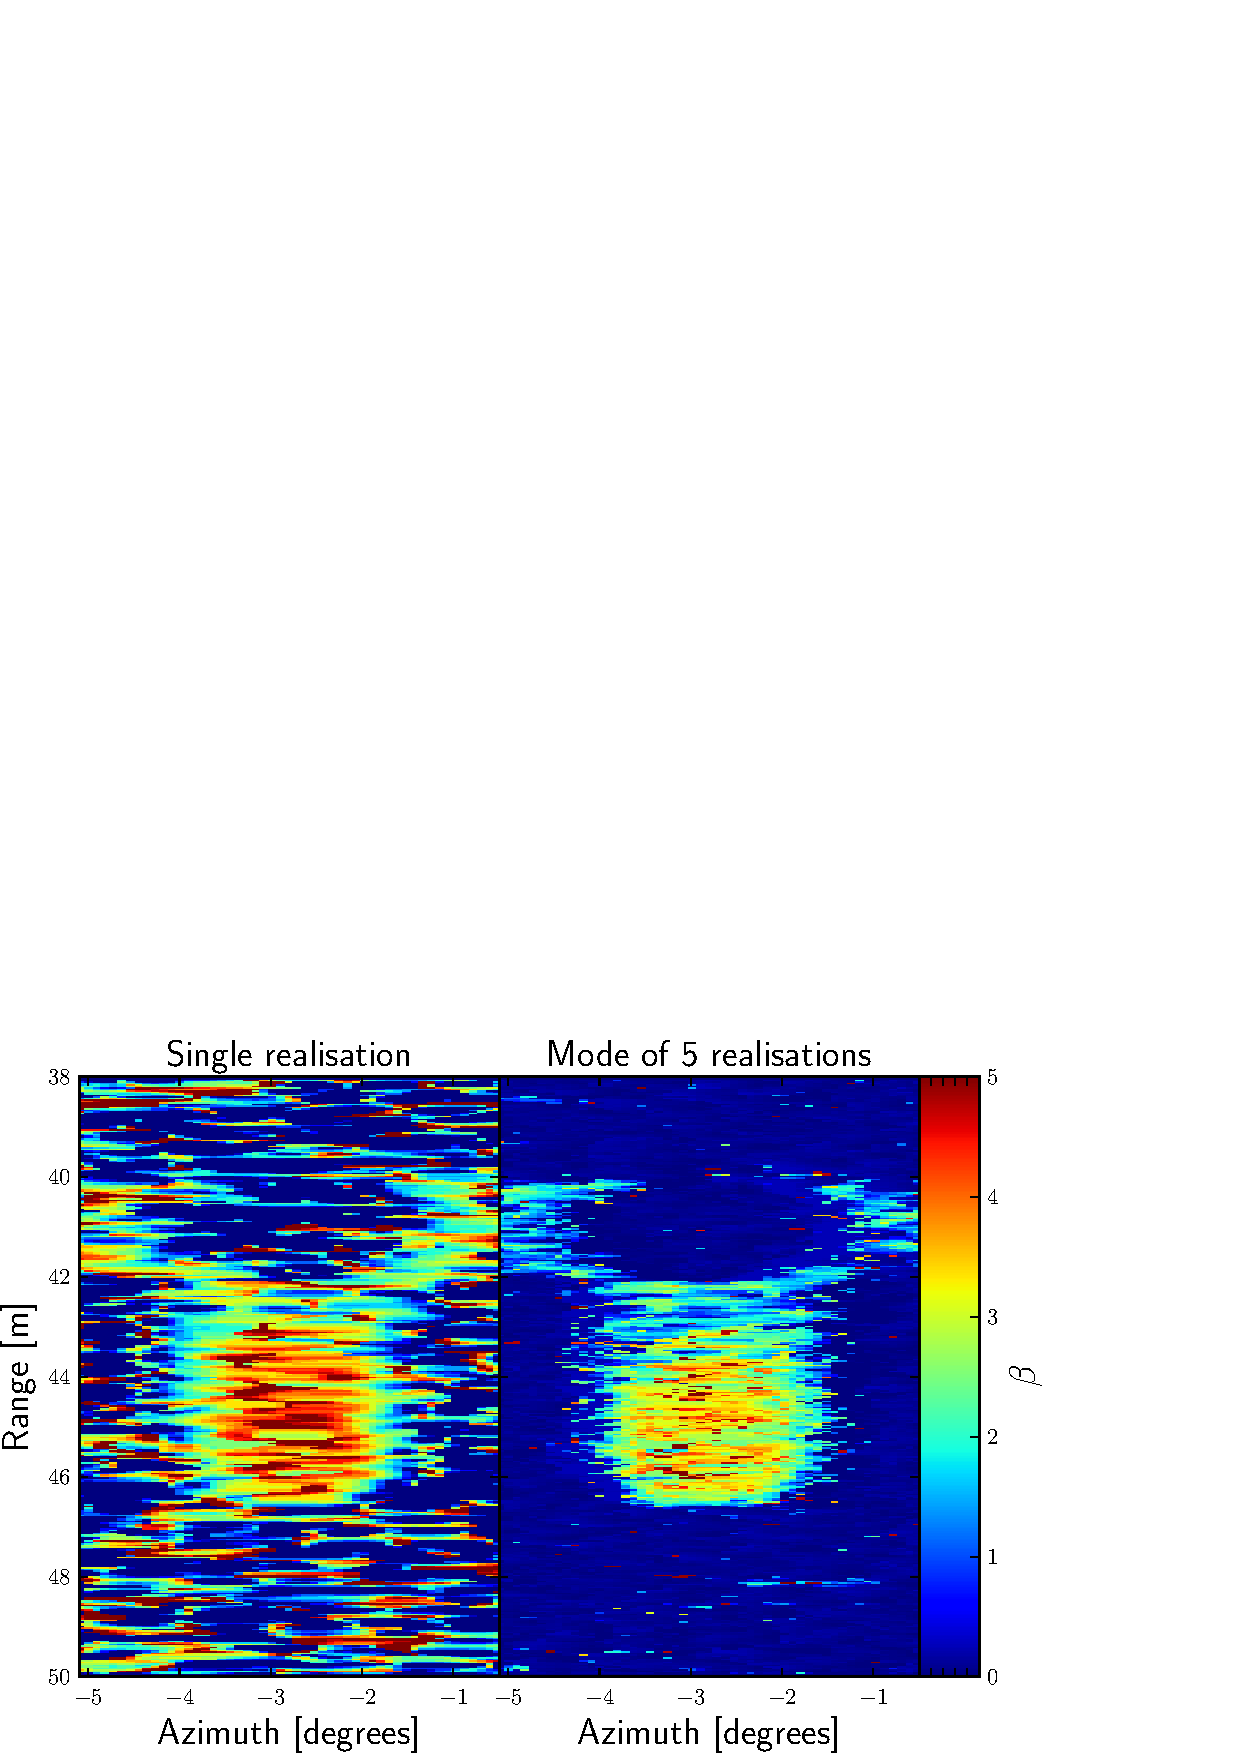
\includegraphics[width=0.49\linewidth]{gfx/7_windows_beta.png}}\hfill
\subfloat[Windows ($\phi$)]{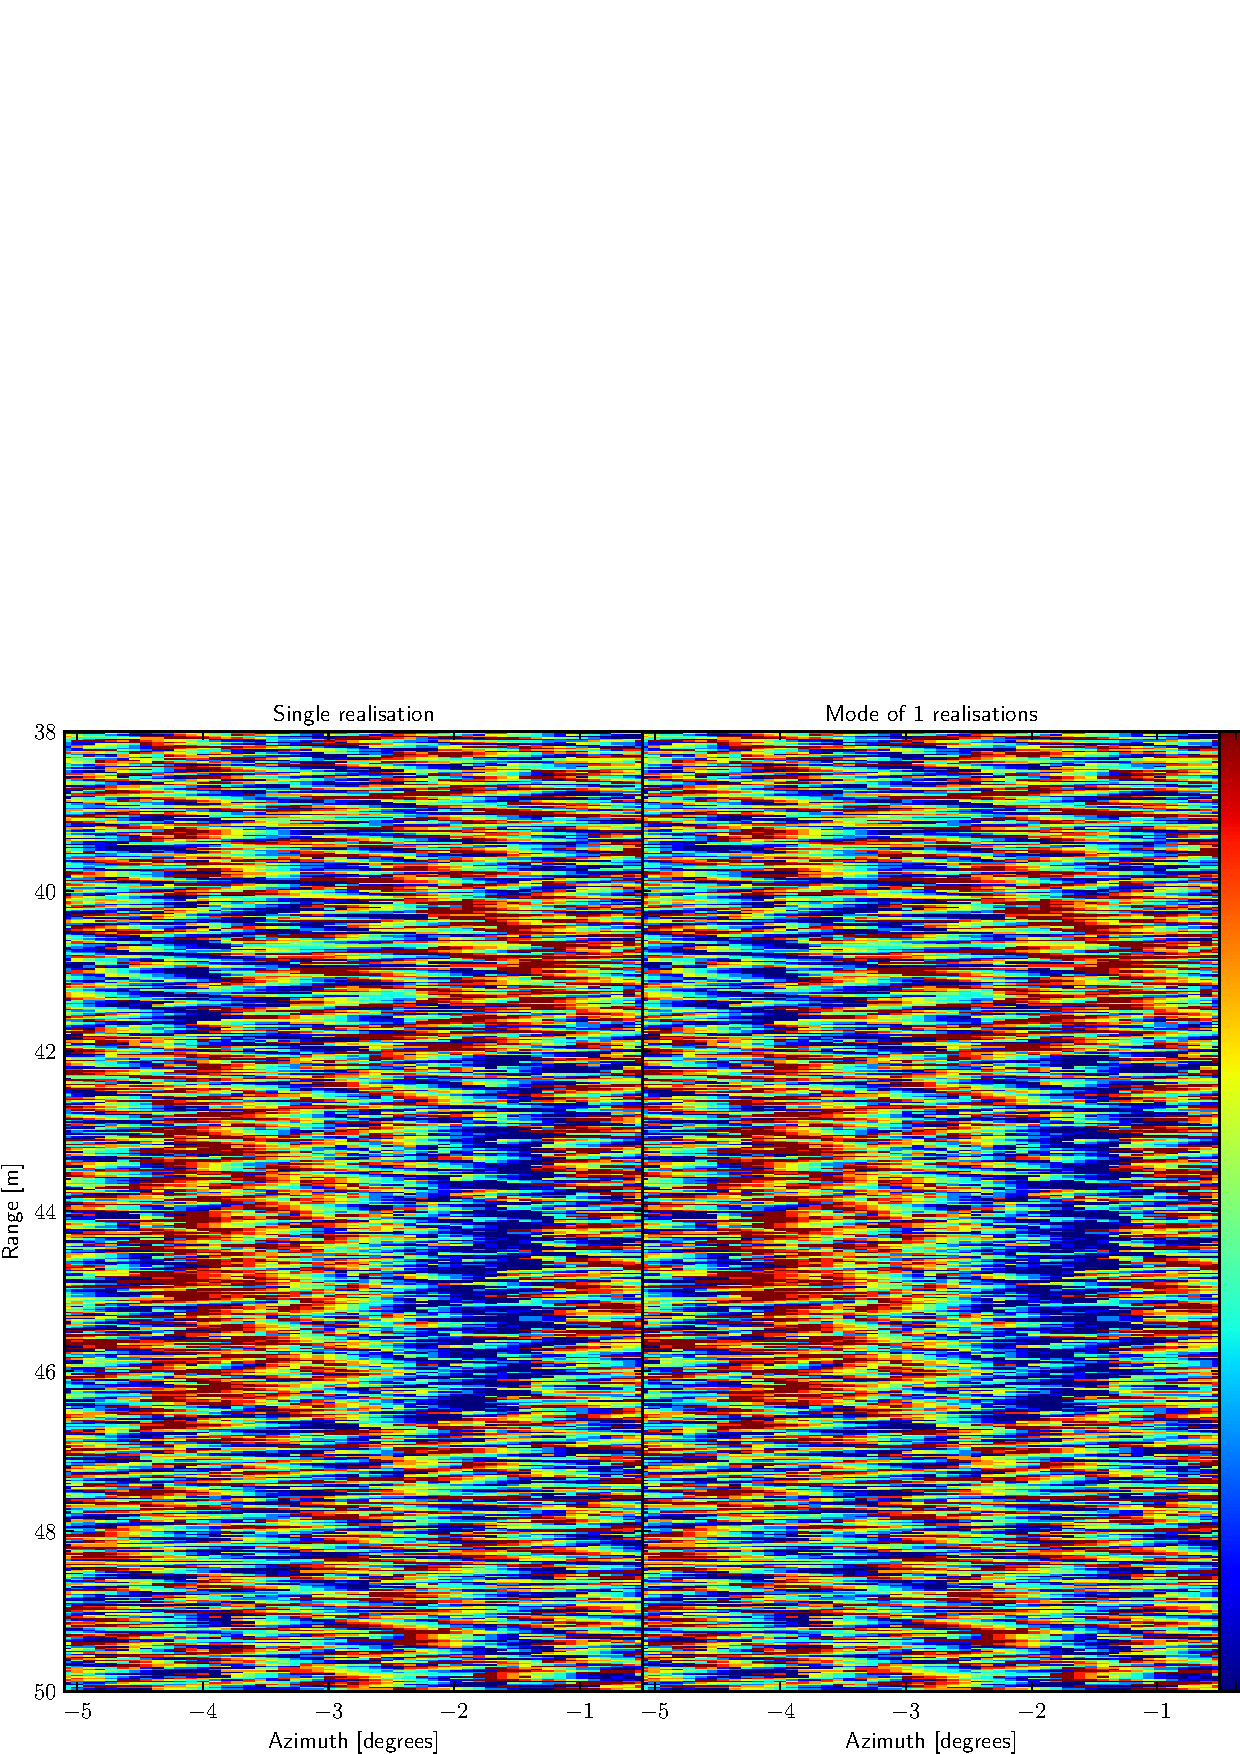
\includegraphics[width=0.48\linewidth]{gfx/7_windows_phi.png}}\\
\subfloat[Capon win. resp. through shadow]{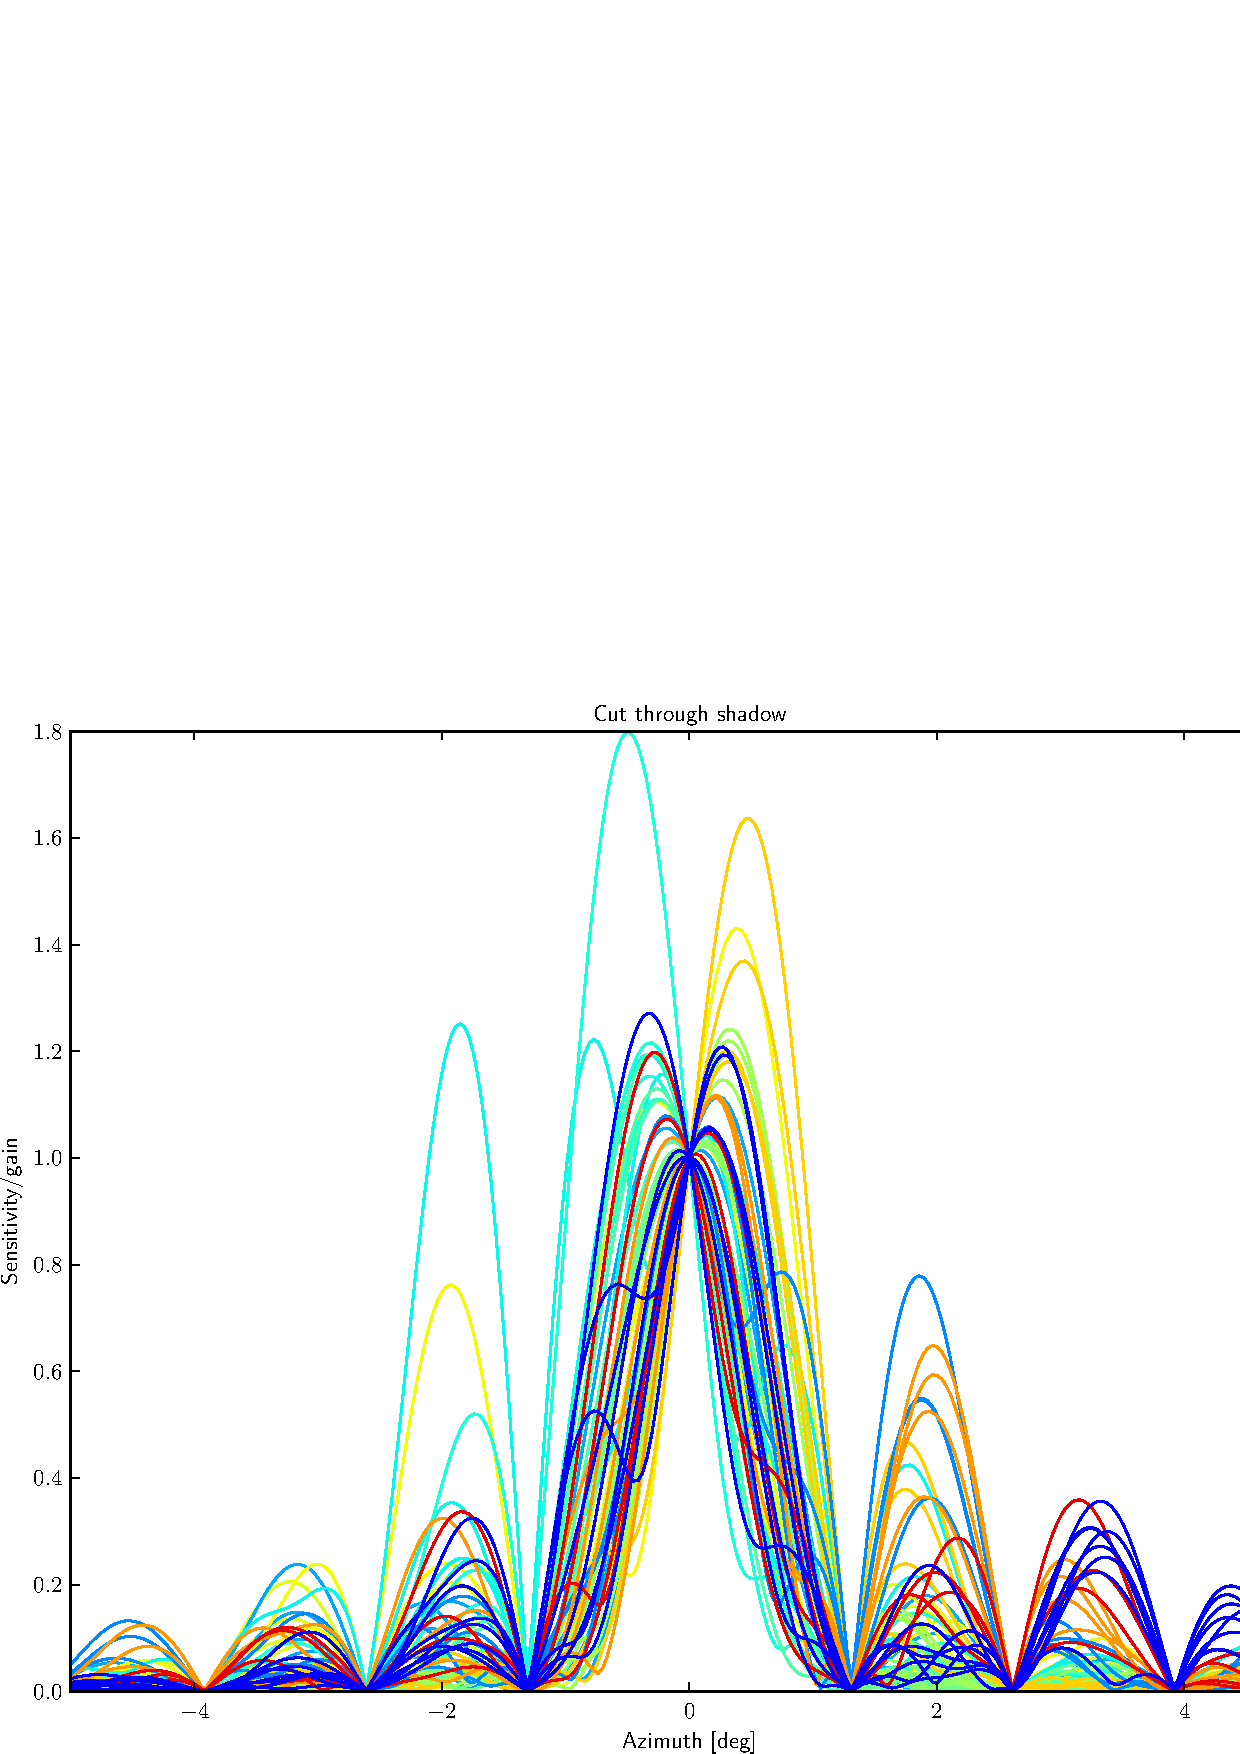
\includegraphics[width=0.49\linewidth]{gfx/7_win_resp_cut_shadow.png}}\hfill
\subfloat[Capon win. resp. through highlight]{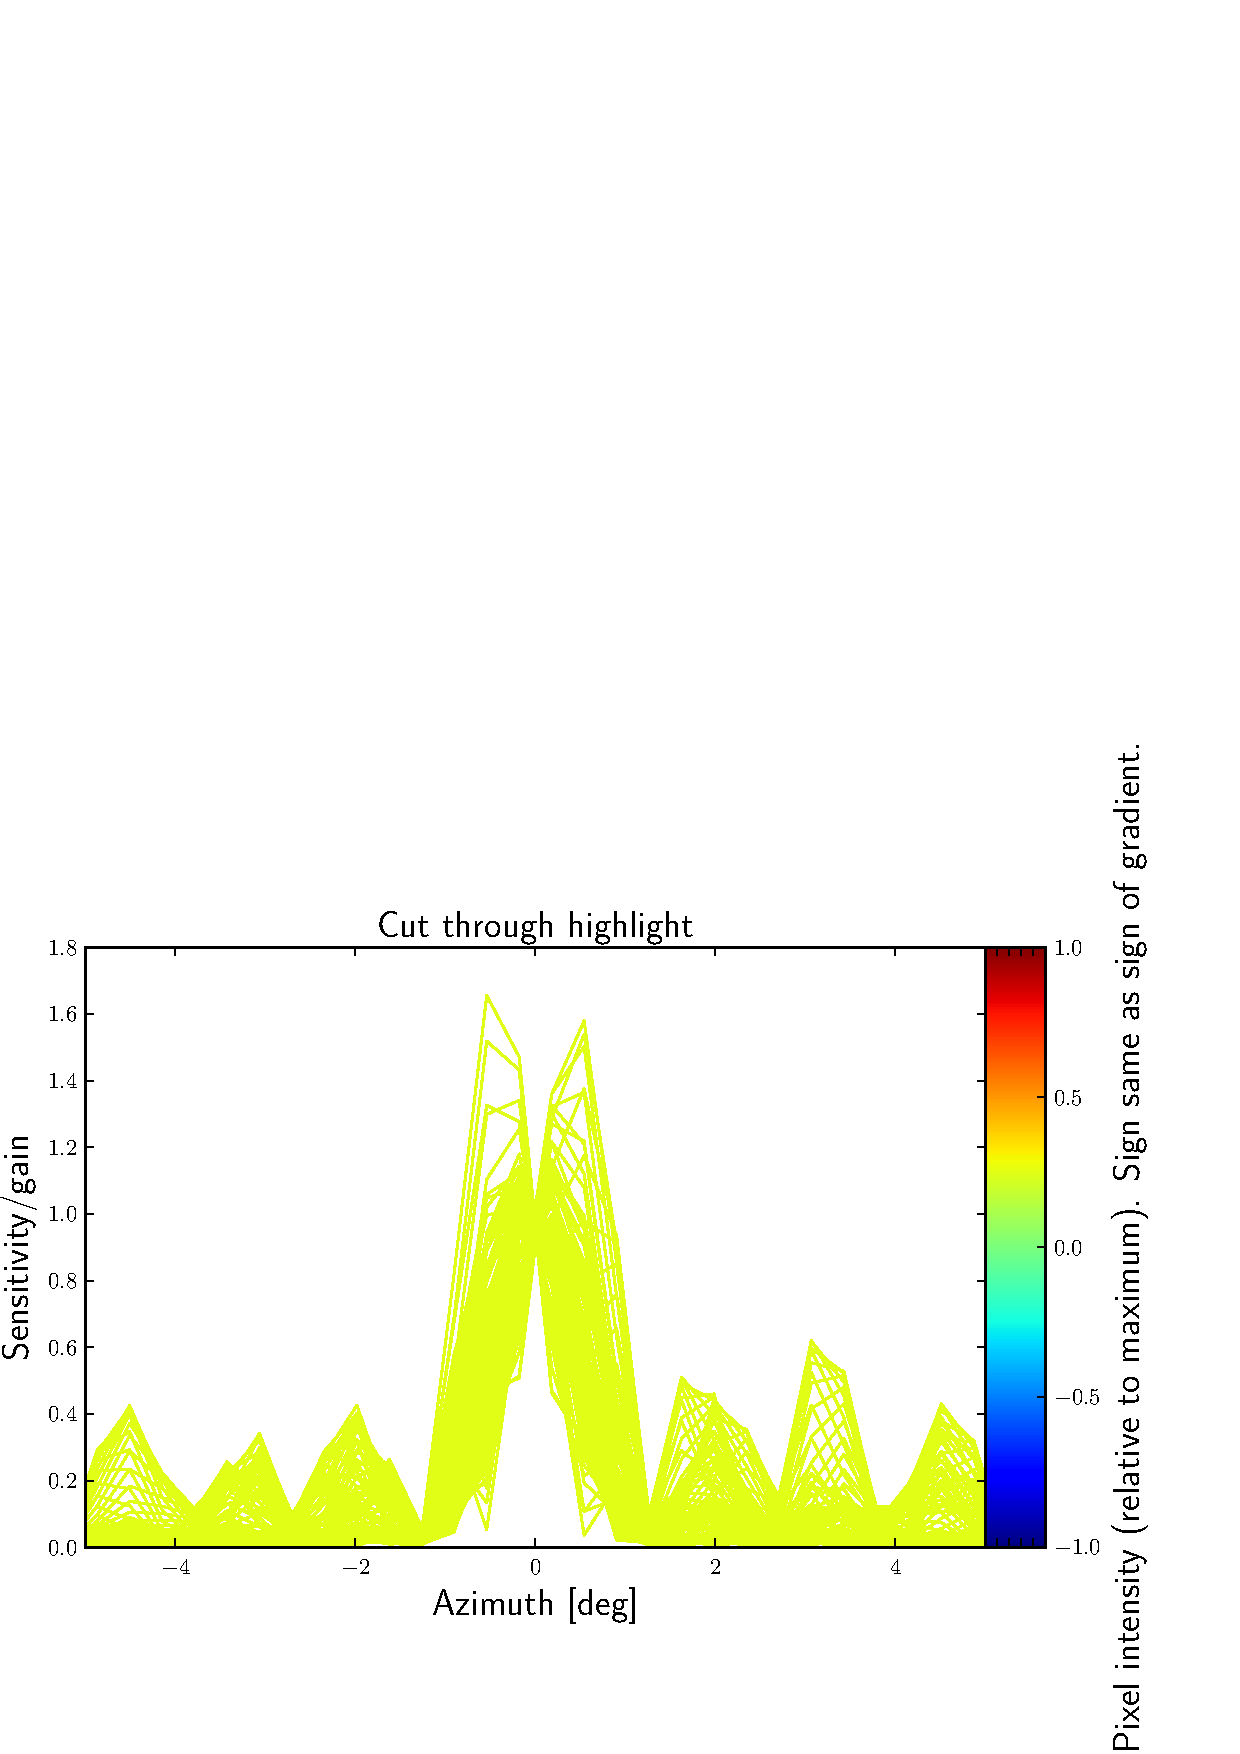
\includegraphics[width=0.49\linewidth]{gfx/7_win_resp_cut_highlight.png}}\\
\end{narrow}
\end{figure*}
\newpage
\begin{figure*}[!t]
\begin{narrow}{-1.2cm}{-1.2cm}\centering\vspace{-1.0cm}
\textbf{8. Capon: Tuning time averaging.}\\
\begin{tabular}[c]{l l l l}
\bf General & M = 32                            & $\Delta r = \frac{c}{2B}$ = 2.5 cm & $\frac{640\,\text{pixels}] / 12\,\text{m}}{\Delta r} = \frac{4}{3}$ \\
\bf LCA     & $\beta \in [0,10]$ (9 values) & $\phi \in [-1.07,1.07]$ deg (9 values) & Navg = 3 \\
\bf Capon   & $\Delta$ = 0.01                 & L = 16                           & Navg = 3 \\
\end{tabular}
\subfloat[LCA Window Response]{\includegraphics[width=0.49\linewidth]{gfx/8_window_response.png}}\hfill
\subfloat[Mean images]{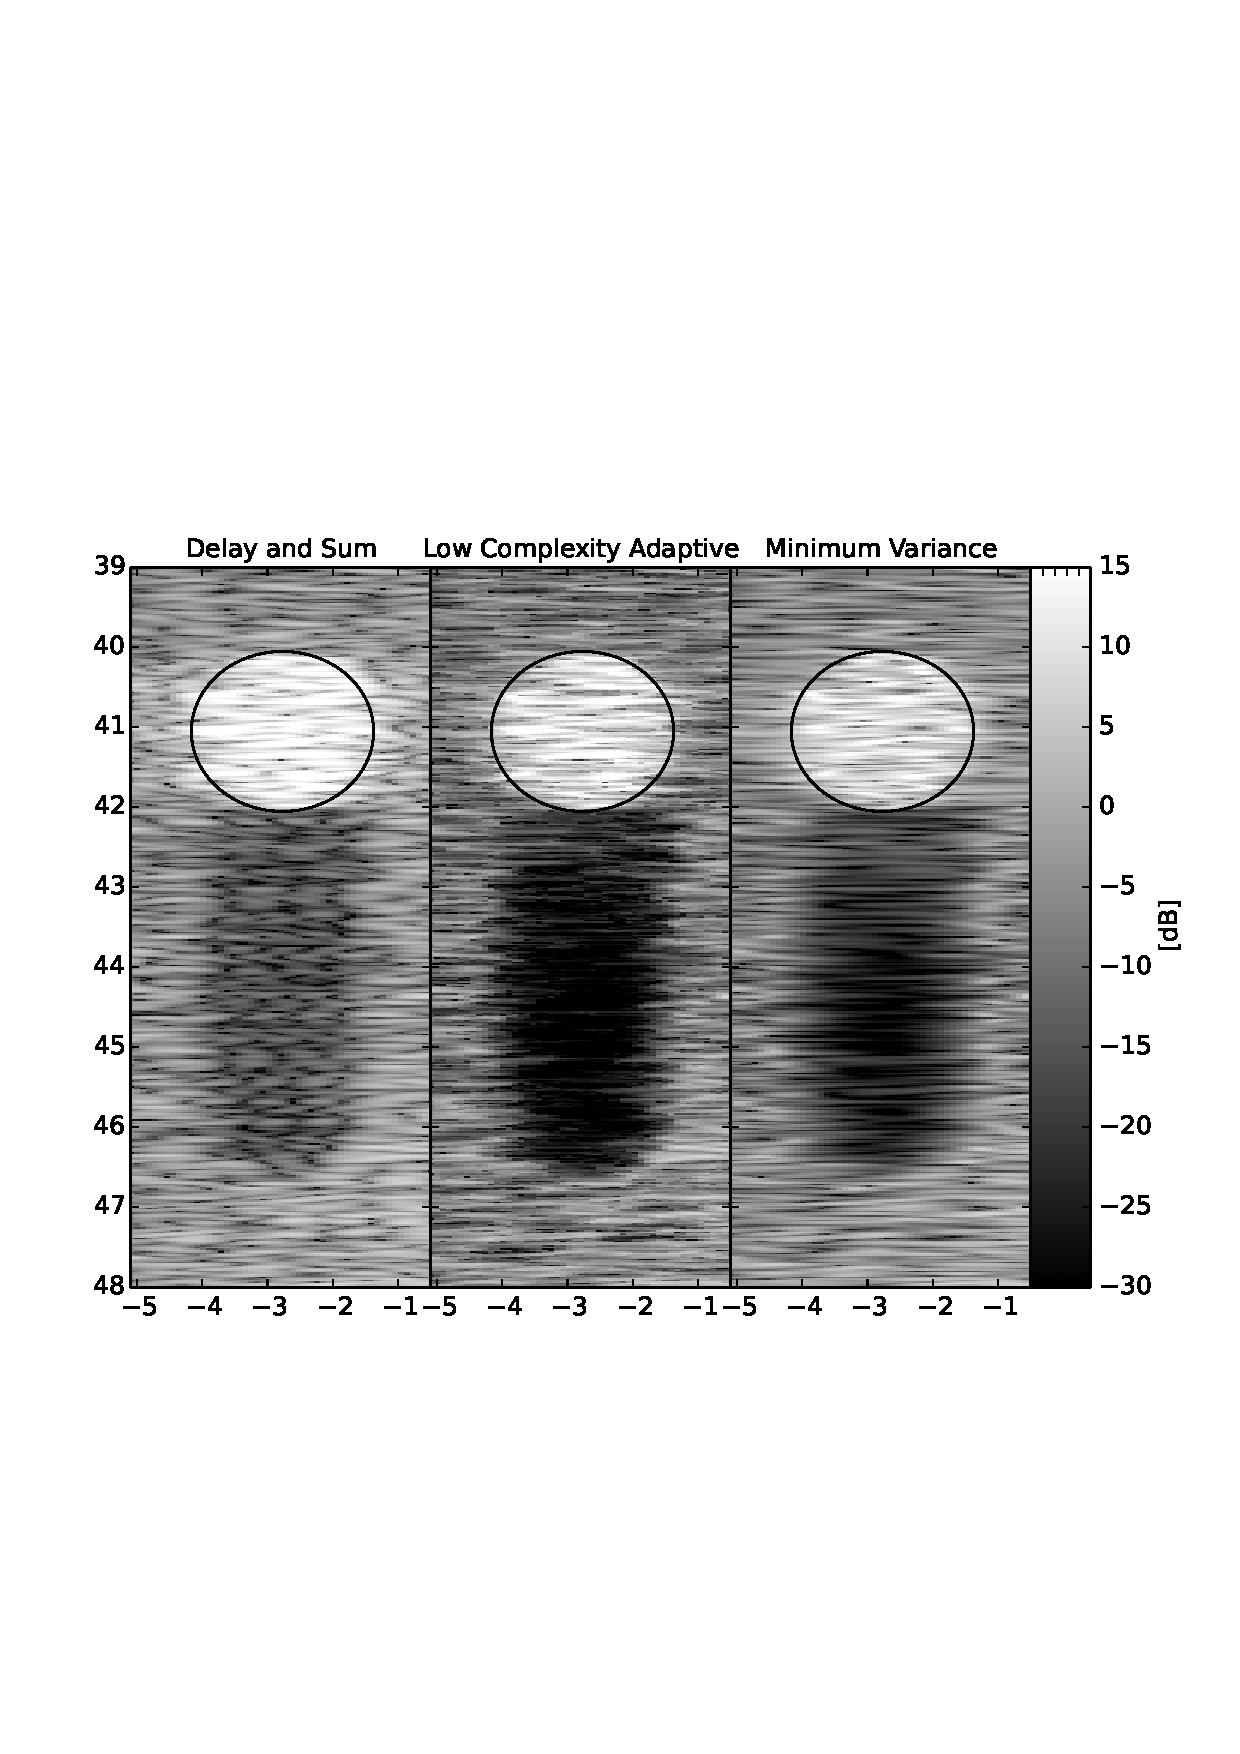
\includegraphics[width=0.49\linewidth]{gfx/8_mean_imgs.png}}\\
\subfloat[Windows ($\beta$)]{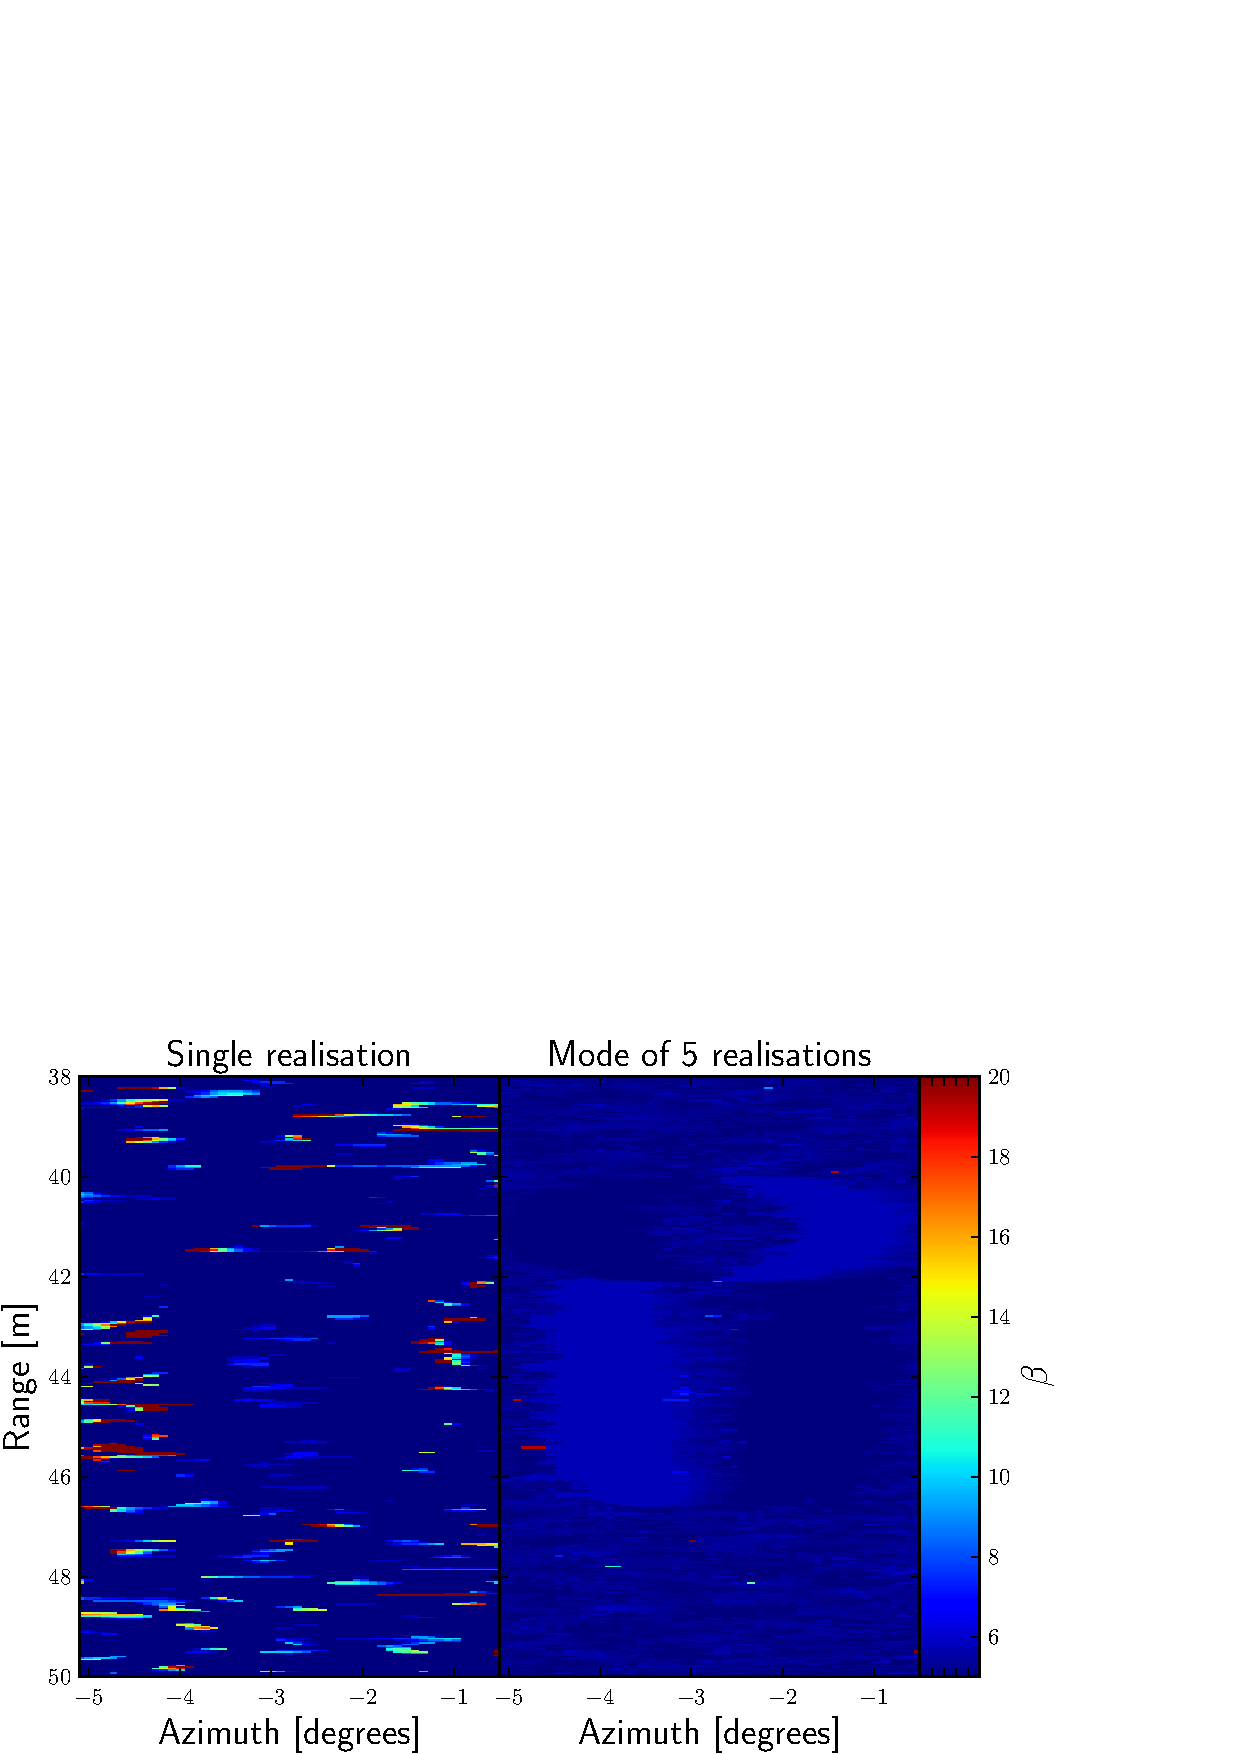
\includegraphics[width=0.49\linewidth]{gfx/8_windows_beta.png}}\hfill
\subfloat[Windows ($\phi$)]{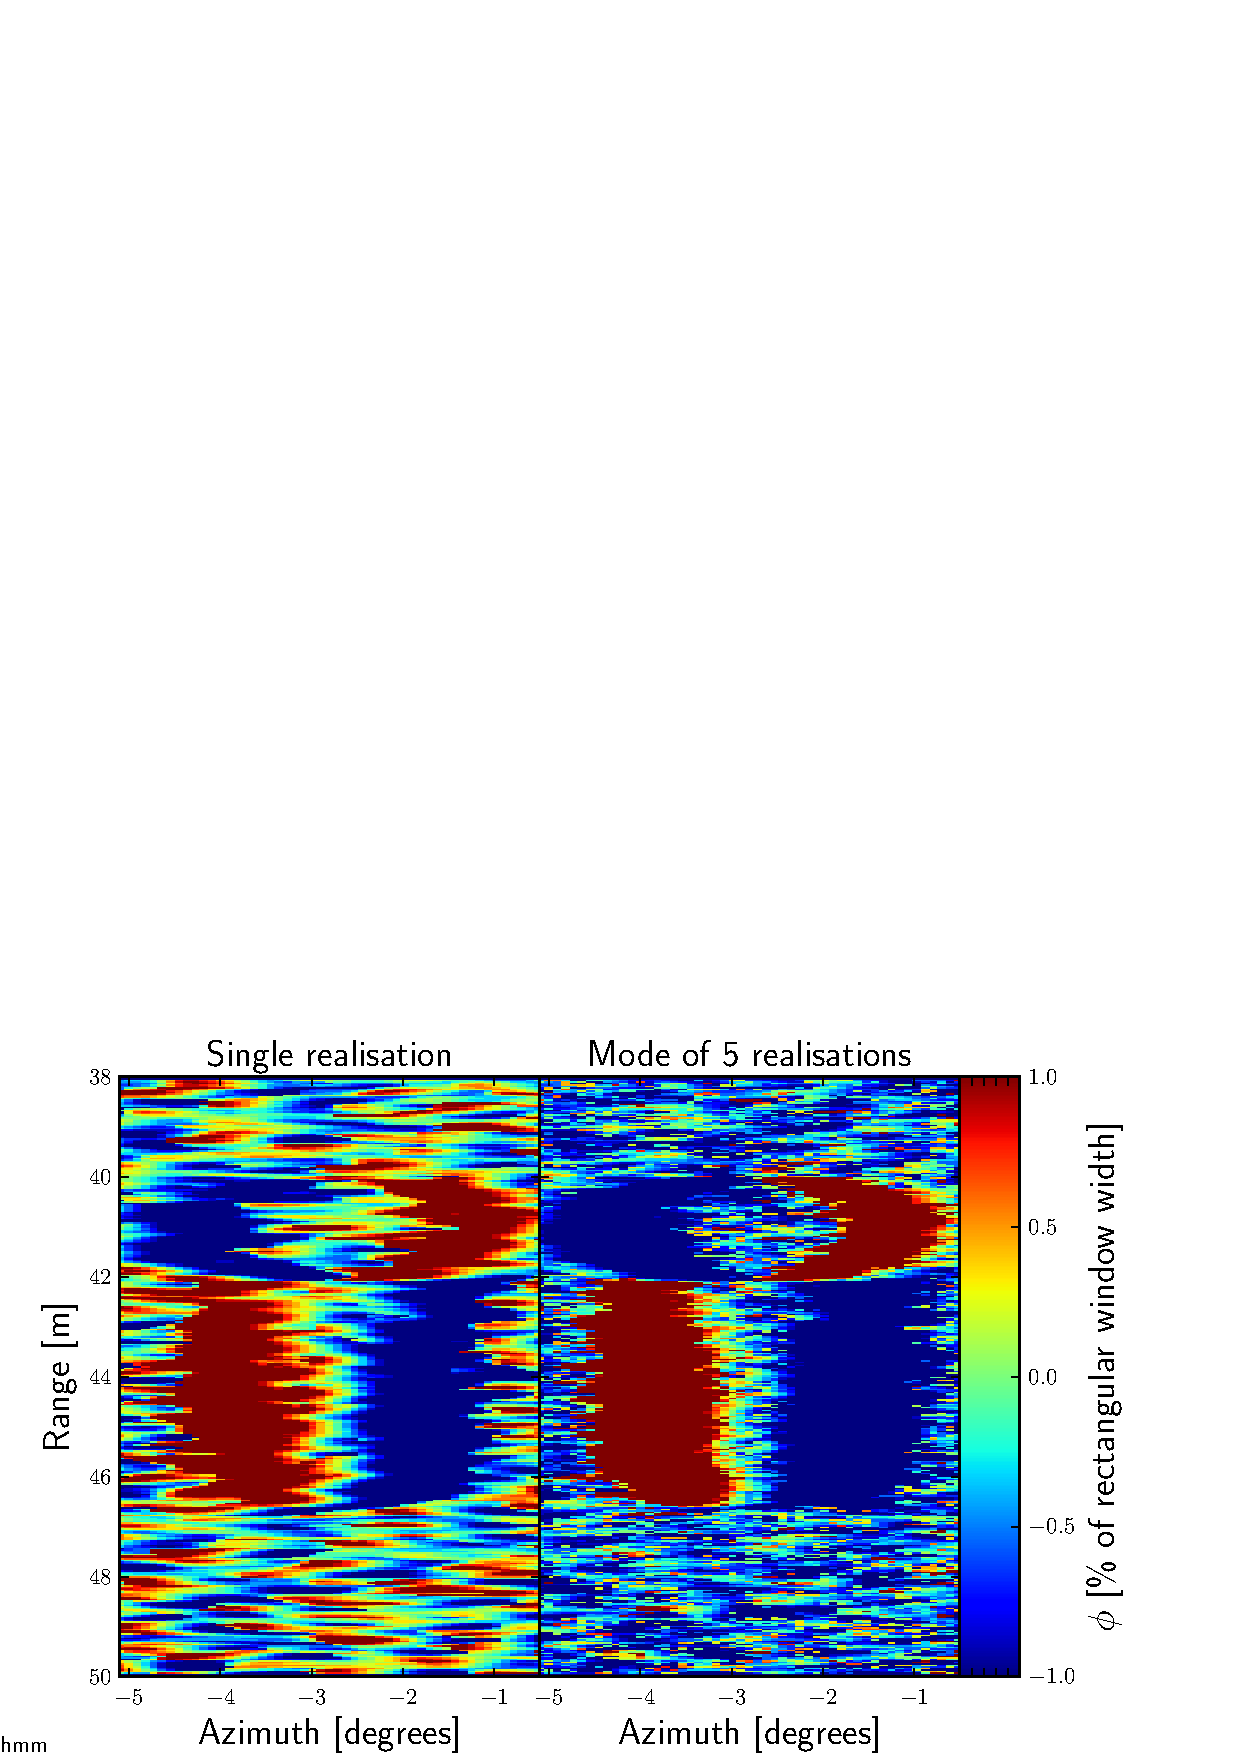
\includegraphics[width=0.48\linewidth]{gfx/8_windows_phi.png}}\\
\subfloat[Capon win. resp. through shadow]{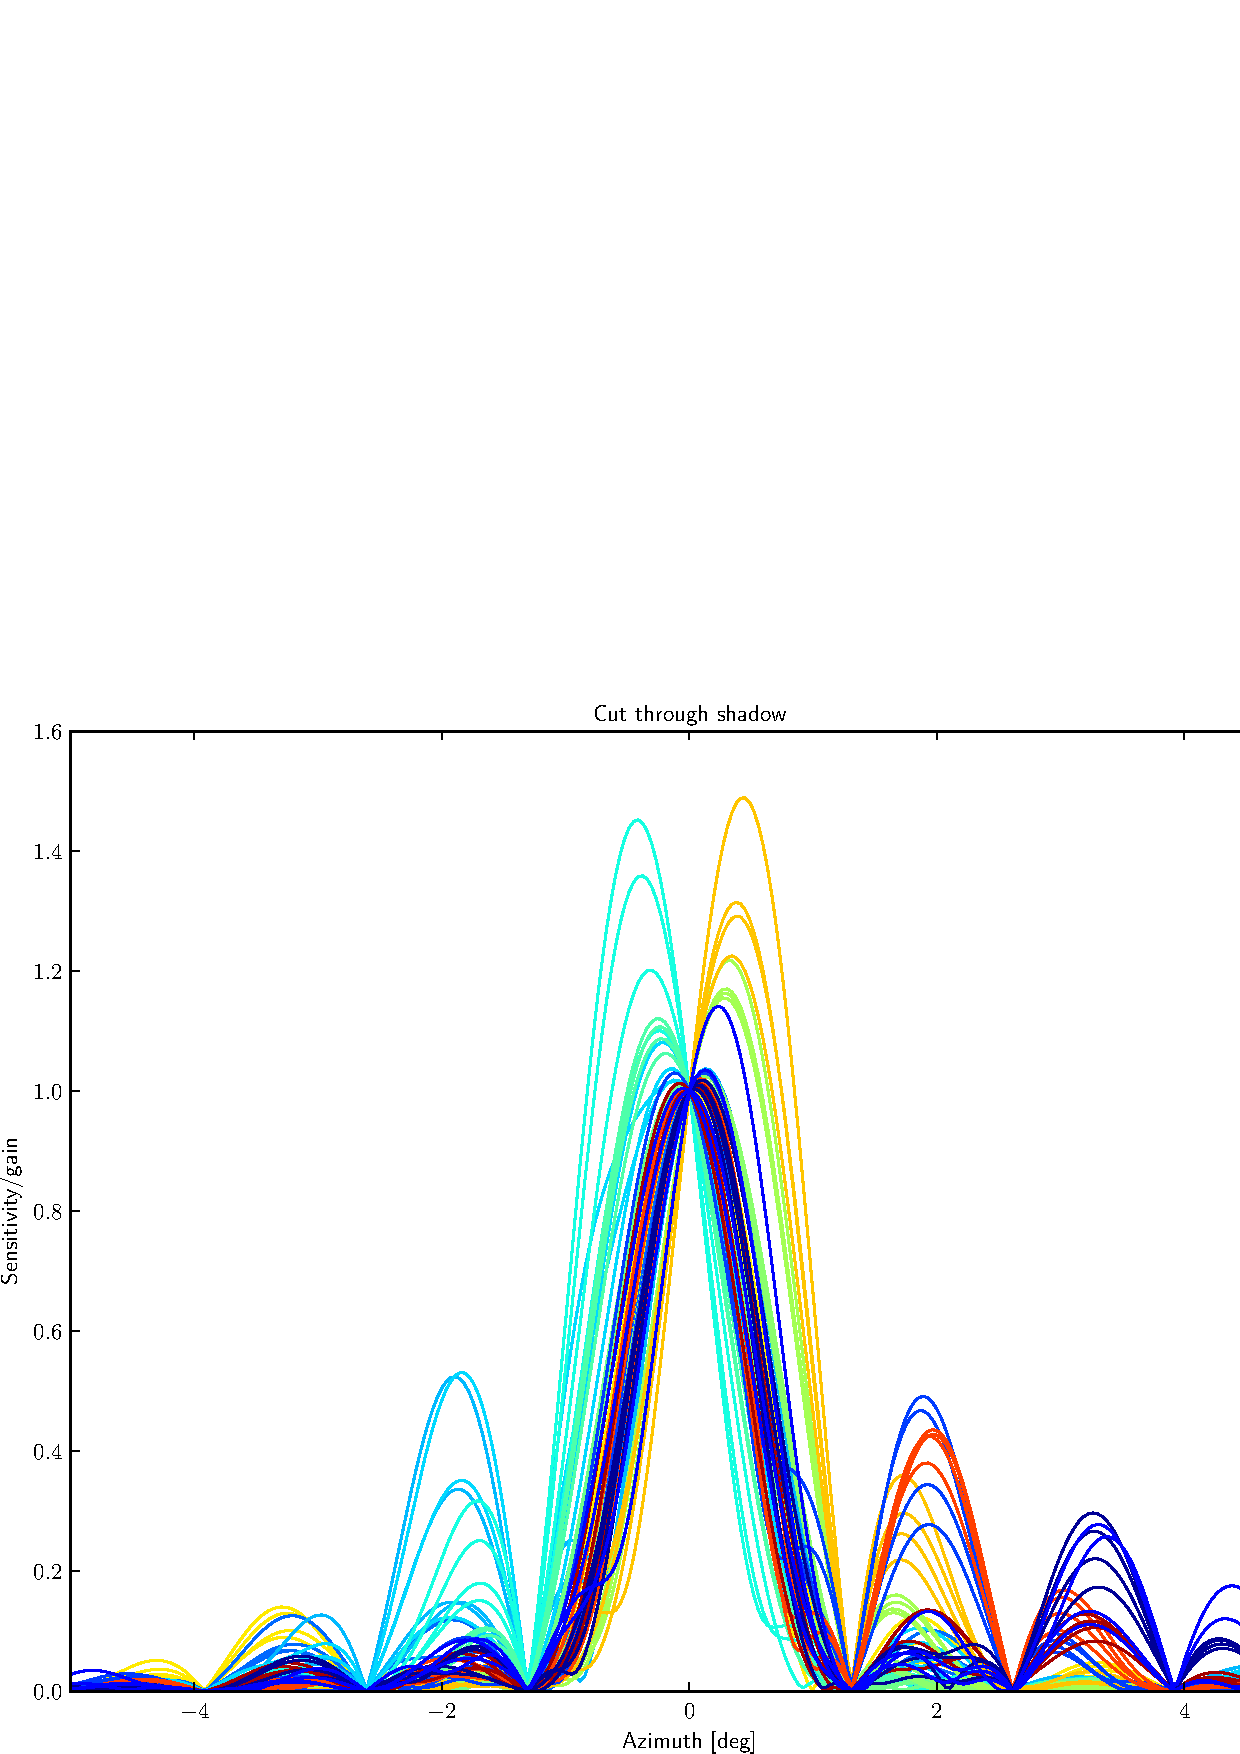
\includegraphics[width=0.49\linewidth]{gfx/8_win_resp_cut_shadow.png}}\hfill
\subfloat[Capon win. resp. through highlight]{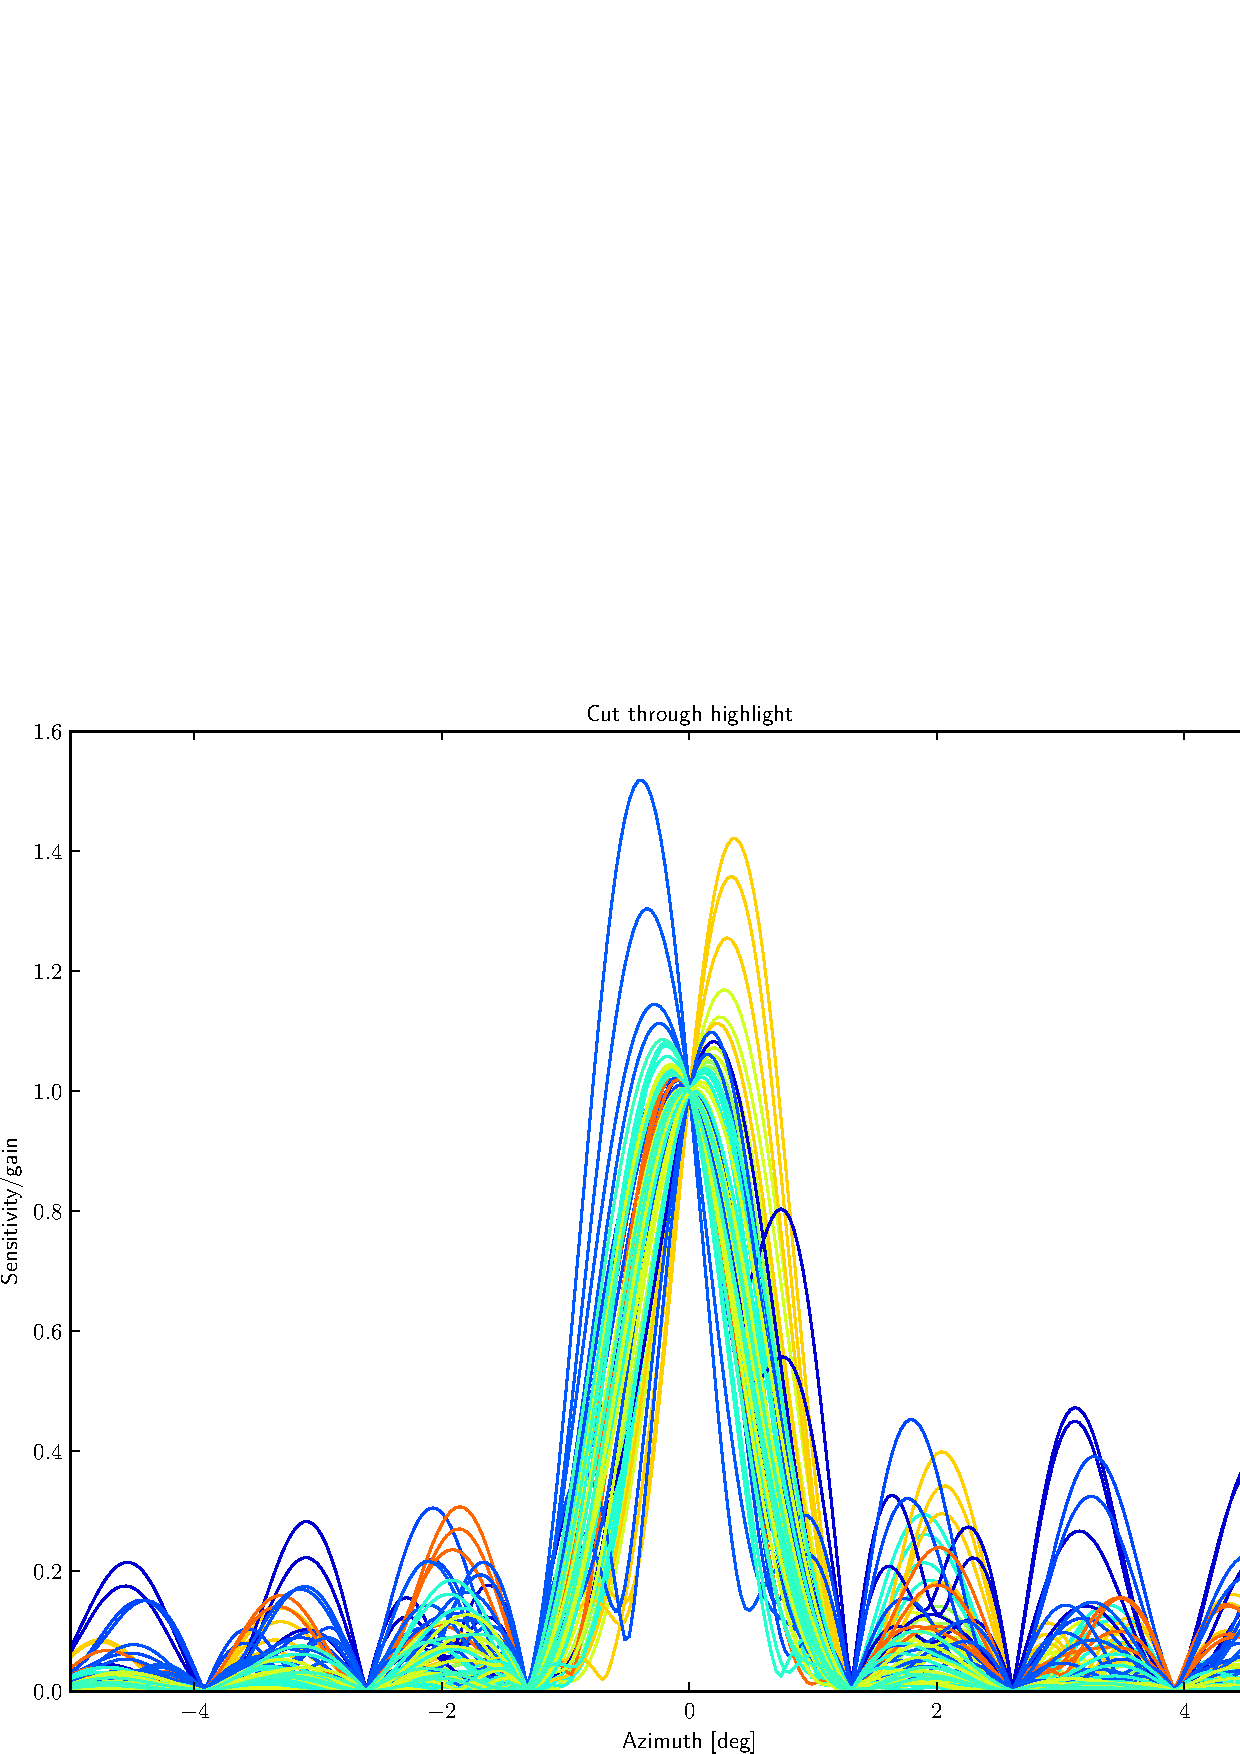
\includegraphics[width=0.49\linewidth]{gfx/8_win_resp_cut_highlight.png}}\\
\end{narrow}
\end{figure*}
\newpage
\begin{figure*}[!t]
\begin{narrow}{-1.2cm}{-1.2cm}\centering\vspace{-1.0cm}
\textbf{9. Capon: Tuning time averaging.}\\
\begin{tabular}[c]{l l l l}
\bf General & M = 32                            & $\Delta r = \frac{c}{2B}$ = 2.5 cm & $\frac{640\,\text{pixels}] / 12\,\text{m}}{\Delta r} = \frac{4}{3}$ \\
\bf LCA     & $\beta \in [0,10]$ (9 values) & $\phi \in [-1.07,1.07]$ deg (9 values) & Navg = 5 \\
\bf Capon   & $\Delta$ = 0.01                 & L = 16                           & Navg = 5 \\
\end{tabular}
\subfloat[LCA Window Response]{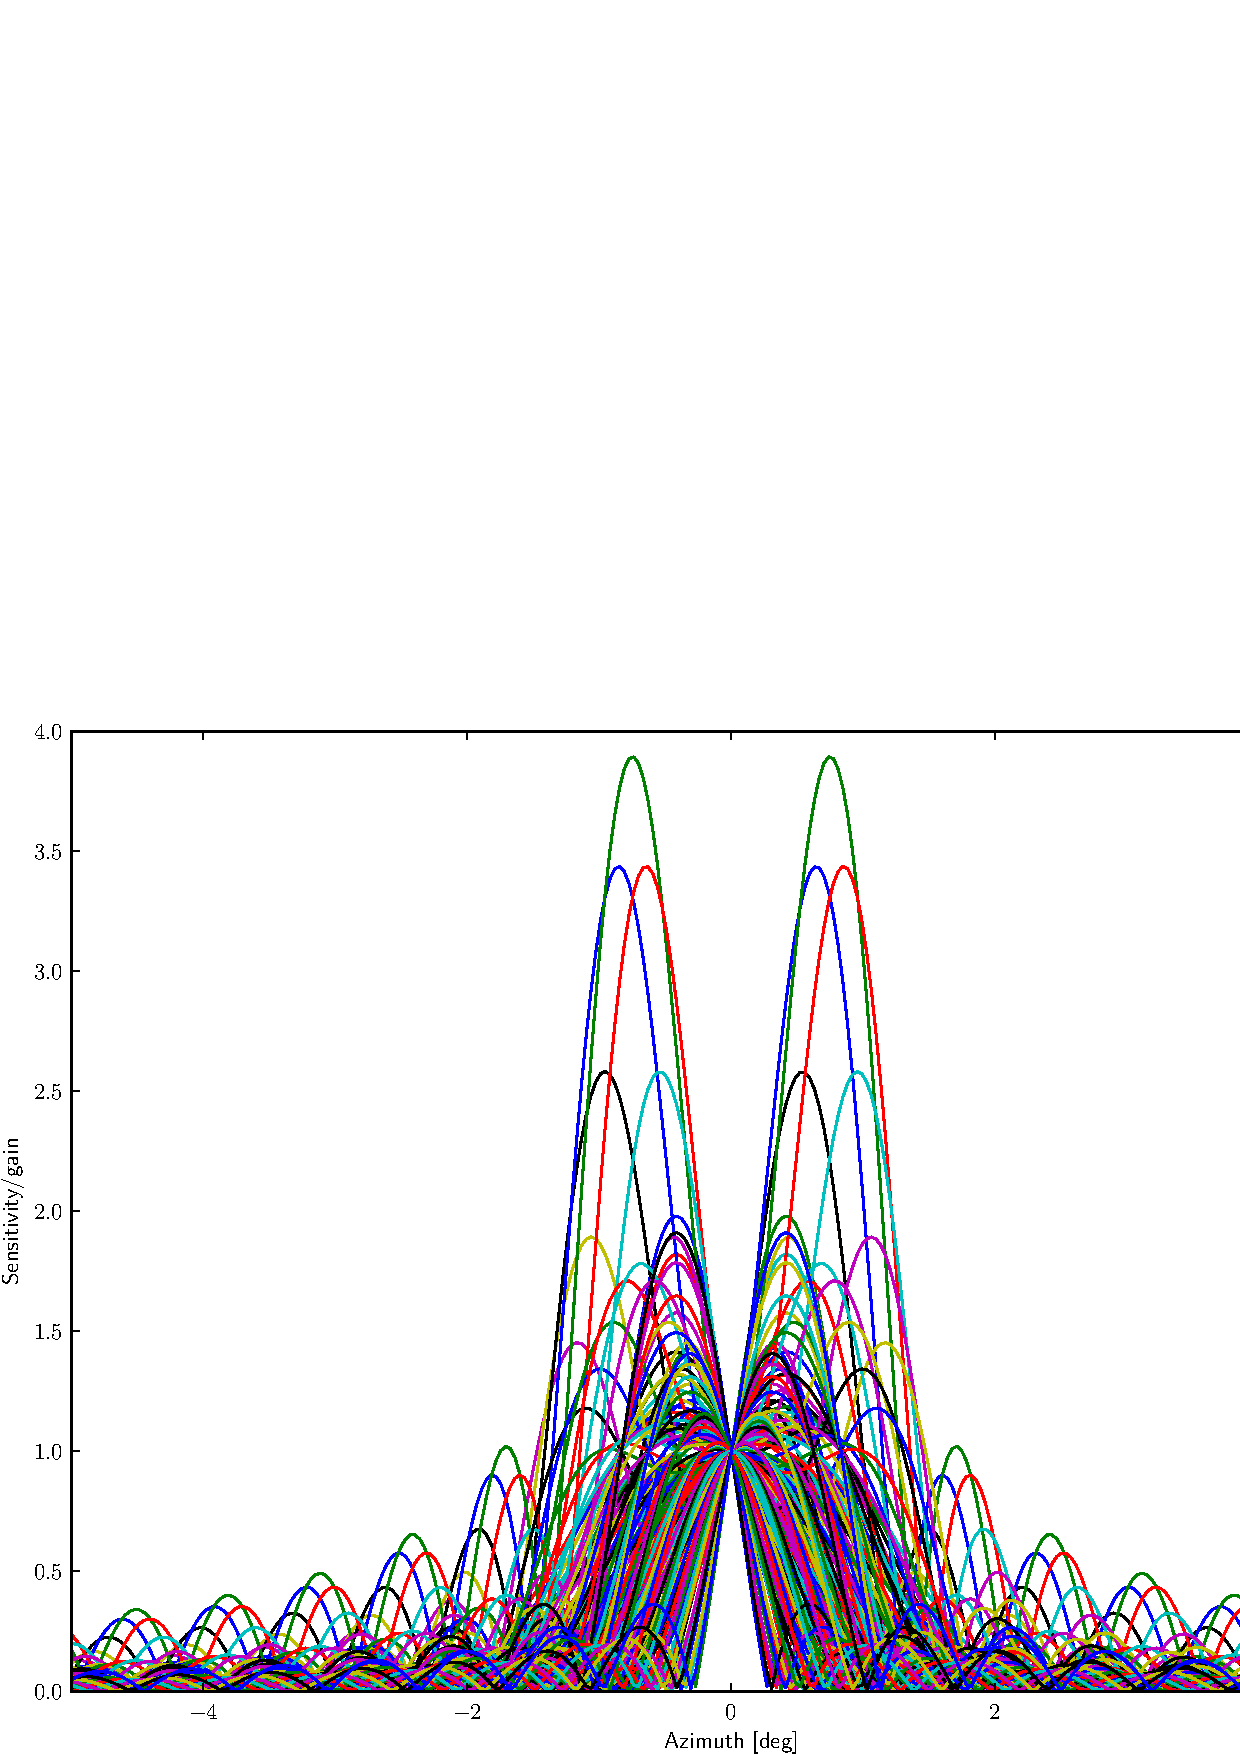
\includegraphics[width=0.49\linewidth]{gfx/9_window_response.png}}\hfill
\subfloat[Mean images]{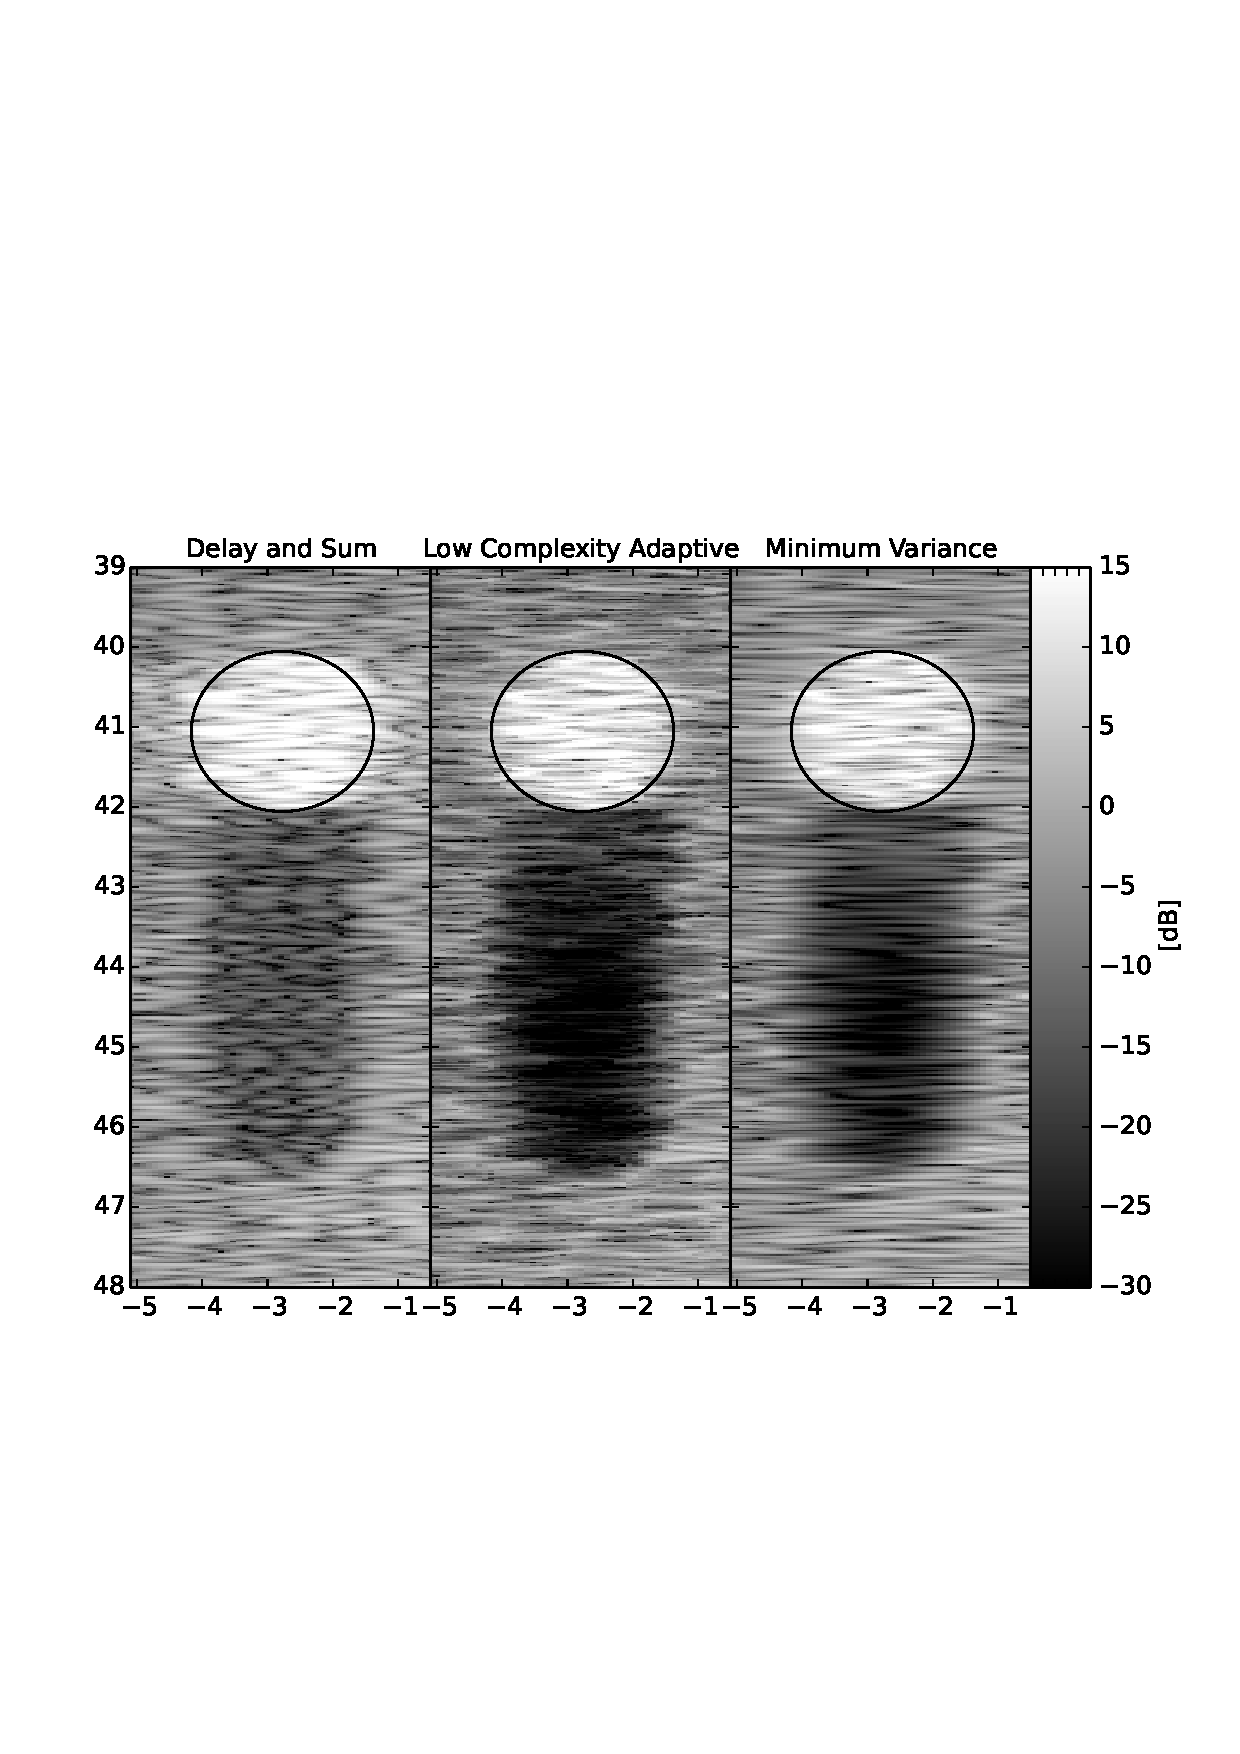
\includegraphics[width=0.49\linewidth]{gfx/9_mean_imgs.png}}\\
\subfloat[Windows ($\beta$)]{\includegraphics[width=0.49\linewidth]{gfx/9_windows_beta.png}}\hfill
\subfloat[Windows ($\phi$)]{\includegraphics[width=0.48\linewidth]{gfx/9_windows_phi.png}}\\
\subfloat[Capon win. resp. through shadow]{\includegraphics[width=0.49\linewidth]{gfx/9_win_resp_cut_shadow.png}}\hfill
\subfloat[Capon win. resp. through highlight]{\includegraphics[width=0.49\linewidth]{gfx/9_win_resp_cut_highlight.png}}\\
\end{narrow}
\end{figure*}
\newpage
\begin{figure*}[!t]
\begin{narrow}{-1.2cm}{-1.2cm}\centering\vspace{-1.0cm}
\textbf{10. Capon: Tuning time averaging.}\\
\begin{tabular}[c]{l l l l}
\bf General & M = 32                            & $\Delta r = \frac{c}{2B}$ = 2.5 cm & $\frac{640\,\text{pixels}] / 12\,\text{m}}{\Delta r} = \frac{4}{3}$ \\
\bf LCA     & $\beta \in [0,10]$ (9 values) & $\phi \in [-1.07,1.07]$ deg (9 values) & Navg = 7 \\
\bf Capon   & $\Delta$ = 0.01                 & L = 16                           & Navg = 7 \\
\end{tabular}
\subfloat[LCA Window Response]{\includegraphics[width=0.49\linewidth]{gfx/10_window_response.png}}\hfill
\subfloat[Mean images]{\includegraphics[width=0.49\linewidth]{gfx/10_mean_imgs.png}}\\
\subfloat[Windows ($\beta$)]{\includegraphics[width=0.49\linewidth]{gfx/10_windows_beta.png}}\hfill
\subfloat[Windows ($\phi$)]{\includegraphics[width=0.48\linewidth]{gfx/10_windows_phi.png}}\\
\subfloat[Capon win. resp. through shadow]{\includegraphics[width=0.49\linewidth]{gfx/10_win_resp_cut_shadow.png}}\hfill
\subfloat[Capon win. resp. through highlight]{\includegraphics[width=0.49\linewidth]{gfx/10_win_resp_cut_highlight.png}}\\
\end{narrow}
\end{figure*}
\newpage
\begin{figure*}[!t]
\begin{narrow}{-1.2cm}{-1.2cm}\centering\vspace{-1.0cm}
\textbf{11. LCA: Reasonable settings.}\\
\begin{tabular}[c]{l l l l}
\bf General & M = 32                            & $\Delta r = \frac{c}{2B}$ = 2.5 cm & $\frac{640\,\text{pixels}] / 12\,\text{m}}{\Delta r} = \frac{4}{3}$ \\
\bf LCA     & $\beta \in [0,10]$ (9 values) & $\phi \in [-0.57,0.57]$ deg (9 values) & Navg = 7 \\
\bf Capon   & $\Delta$ = 0.01                 & L = 16                           & Navg = 7 \\
\end{tabular}
\subfloat[LCA Window Response]{\includegraphics[width=0.49\linewidth]{gfx/11_window_response.png}}\hfill
\subfloat[Mean images]{\includegraphics[width=0.49\linewidth]{gfx/11_mean_imgs.png}}\\
\subfloat[Windows ($\beta$)]{\includegraphics[width=0.49\linewidth]{gfx/11_windows_beta.png}}\hfill
\subfloat[Windows ($\phi$)]{\includegraphics[width=0.48\linewidth]{gfx/11_windows_phi.png}}\\
\subfloat[Capon win. resp. through shadow]{\includegraphics[width=0.49\linewidth]{gfx/11_win_resp_cut_shadow.png}}\hfill
\subfloat[Capon win. resp. through highlight]{\includegraphics[width=0.49\linewidth]{gfx/11_win_resp_cut_highlight.png}}\\
\end{narrow}
\end{figure*}
\newpage
\begin{figure*}[!t]
\begin{narrow}{-1.2cm}{-1.2cm}\centering\vspace{-1.0cm}
\textbf{12. LCA: Lots of Kaiser windows - wide span.}\\
\begin{tabular}[c]{l l l l}
\bf General & M = 32                            & $\Delta r = \frac{c}{2B}$ = 2.5 cm & $\frac{640\,\text{pixels}] / 12\,\text{m}}{\Delta r} = \frac{4}{3}$ \\
\bf LCA     & $\beta \in [0,20]$ (19 values) & $\phi \in [-1.07,1.07]$ deg (19 values) & Navg = 7 \\
\bf Capon   & $\Delta$ = 0.01                 & L = 16                           & Navg = 7 \\
\end{tabular}
\subfloat[LCA Window Response]{\includegraphics[width=0.49\linewidth]{gfx/12_window_response.png}}\hfill
\subfloat[Mean images]{\includegraphics[width=0.49\linewidth]{gfx/12_mean_imgs.png}}\\
\subfloat[Windows ($\beta$)]{\includegraphics[width=0.49\linewidth]{gfx/12_windows_beta.png}}\hfill
\subfloat[Windows ($\phi$)]{\includegraphics[width=0.48\linewidth]{gfx/12_windows_phi.png}}\\
\subfloat[Capon win. resp. through shadow]{\includegraphics[width=0.49\linewidth]{gfx/12_win_resp_cut_shadow.png}}\hfill
\subfloat[Capon win. resp. through highlight]{\includegraphics[width=0.49\linewidth]{gfx/12_win_resp_cut_highlight.png}}\\
\end{narrow}
\end{figure*}
\newpage
\begin{figure*}[!t]
\begin{narrow}{-1.2cm}{-1.2cm}\centering\vspace{-1.0cm}
\textbf{13. LCA: Lots of trigonometric windows - wide span.}\\
\begin{tabular}[c]{l l l l}
\bf General & M = 32                            & $\Delta r = \frac{c}{2B}$ = 2.5 cm & $\frac{640\,\text{pixels}] / 12\,\text{m}}{\Delta r} = \frac{4}{3}$ \\
\bf LCA     & $\beta \in [0,20]$ (19 values) & $\phi \in [-1.07,1.07]$ deg (19 values) & Navg = 7 \\
\bf Capon   & $\Delta$ = 0.01                 & L = 16                           & Navg = 7 \\
\end{tabular}
\subfloat[LCA Window Response]{\includegraphics[width=0.49\linewidth]{gfx/13_window_response.png}}\hfill
\subfloat[Mean images]{\includegraphics[width=0.49\linewidth]{gfx/13_mean_imgs.png}}\\
\subfloat[Windows ($\beta$)]{\includegraphics[width=0.49\linewidth]{gfx/13_windows_beta.png}}\hfill
\subfloat[Windows ($\phi$)]{\includegraphics[width=0.48\linewidth]{gfx/13_windows_phi.png}}\\
\subfloat[Capon win. resp. through shadow]{\includegraphics[width=0.49\linewidth]{gfx/13_win_resp_cut_shadow.png}}\hfill
\subfloat[Capon win. resp. through highlight]{\includegraphics[width=0.49\linewidth]{gfx/13_win_resp_cut_highlight.png}}\\
\end{narrow}
\end{figure*}
\newpage
\begin{figure*}[!t]
\begin{narrow}{-1.2cm}{-1.2cm}\centering\vspace{-1.0cm}
\textbf{14. LCA: Back on Kaiser - reducing steering span.}\\
\begin{tabular}[c]{l l l l}
\bf General & M = 32                            & $\Delta r = \frac{c}{2B}$ = 2.5 cm & $\frac{640\,\text{pixels}] / 12\,\text{m}}{\Delta r} = \frac{4}{3}$ \\
\bf LCA     & $\beta \in [0,20]$ (19 values) & $\phi \in [-0.72,0.72]$ deg (19 values) & Navg = 7 \\
\bf Capon   & $\Delta$ = 0.01                 & L = 16                           & Navg = 7 \\
\end{tabular}
\subfloat[LCA Window Response]{\includegraphics[width=0.49\linewidth]{gfx/14_window_response.png}}\hfill
\subfloat[Mean images]{\includegraphics[width=0.49\linewidth]{gfx/14_mean_imgs.png}}\\
\subfloat[Windows ($\beta$)]{\includegraphics[width=0.49\linewidth]{gfx/14_windows_beta.png}}\hfill
\subfloat[Windows ($\phi$)]{\includegraphics[width=0.48\linewidth]{gfx/14_windows_phi.png}}\\
\subfloat[Capon win. resp. through shadow]{\includegraphics[width=0.49\linewidth]{gfx/14_win_resp_cut_shadow.png}}\hfill
\subfloat[Capon win. resp. through highlight]{\includegraphics[width=0.49\linewidth]{gfx/14_win_resp_cut_highlight.png}}\\
\end{narrow}
\end{figure*}
\newpage
\begin{figure*}[!t]
\begin{narrow}{-1.2cm}{-1.2cm}\centering\vspace{-1.0cm}
\textbf{15. LCA: Reducing steering span.}\\
\begin{tabular}[c]{l l l l}
\bf General & M = 32                            & $\Delta r = \frac{c}{2B}$ = 2.5 cm & $\frac{640\,\text{pixels}] / 12\,\text{m}}{\Delta r} = \frac{4}{3}$ \\
\bf LCA     & $\beta \in [0,20]$ (19 values) & $\phi \in [-0.36,0.36]$ deg (19 values) & Navg = 7 \\
\bf Capon   & $\Delta$ = 0.01                 & L = 16                           & Navg = 7 \\
\end{tabular}
\subfloat[LCA Window Response]{\includegraphics[width=0.49\linewidth]{gfx/15_window_response.png}}\hfill
\subfloat[Mean images]{\includegraphics[width=0.49\linewidth]{gfx/15_mean_imgs.png}}\\
\subfloat[Windows ($\beta$)]{\includegraphics[width=0.49\linewidth]{gfx/15_windows_beta.png}}\hfill
\subfloat[Windows ($\phi$)]{\includegraphics[width=0.48\linewidth]{gfx/15_windows_phi.png}}\\
\subfloat[Capon win. resp. through shadow]{\includegraphics[width=0.49\linewidth]{gfx/15_win_resp_cut_shadow.png}}\hfill
\subfloat[Capon win. resp. through highlight]{\includegraphics[width=0.49\linewidth]{gfx/15_win_resp_cut_highlight.png}}\\
\end{narrow}
\end{figure*}
\newpage
\begin{figure*}[!t]
\begin{narrow}{-1.2cm}{-1.2cm}\centering\vspace{-1.0cm}
\textbf{16. LCA: Adjusting resolution/SNR.}\\
\begin{tabular}[c]{l l l l}
\bf General & M = 32                            & $\Delta r = \frac{c}{2B}$ = 2.5 cm & $\frac{640\,\text{pixels}] / 12\,\text{m}}{\Delta r} = \frac{4}{3}$ \\
\bf LCA     & $\beta \in [0,5]$ (19 values) & $\phi \in [-0.72,0.72]$ deg (19 values) & Navg = 7 \\
\bf Capon   & $\Delta$ = 0.01                 & L = 16                           & Navg = 7 \\
\end{tabular}
\subfloat[LCA Window Response]{\includegraphics[width=0.49\linewidth]{gfx/16_window_response.png}}\hfill
\subfloat[Mean images]{\includegraphics[width=0.49\linewidth]{gfx/16_mean_imgs.png}}\\
\subfloat[Windows ($\beta$)]{\includegraphics[width=0.49\linewidth]{gfx/16_windows_beta.png}}\hfill
\subfloat[Windows ($\phi$)]{\includegraphics[width=0.48\linewidth]{gfx/16_windows_phi.png}}\\
\subfloat[Capon win. resp. through shadow]{\includegraphics[width=0.49\linewidth]{gfx/16_win_resp_cut_shadow.png}}\hfill
\subfloat[Capon win. resp. through highlight]{\includegraphics[width=0.49\linewidth]{gfx/16_win_resp_cut_highlight.png}}\\
\end{narrow}
\end{figure*}
\newpage
\begin{figure*}[!t]
\begin{narrow}{-1.2cm}{-1.2cm}\centering\vspace{-1.0cm}
\textbf{17. LCA: Adjusting resolution/SNR.}\\
\begin{tabular}[c]{l l l l}
\bf General & M = 32                            & $\Delta r = \frac{c}{2B}$ = 2.5 cm & $\frac{640\,\text{pixels}] / 12\,\text{m}}{\Delta r} = \frac{4}{3}$ \\
\bf LCA     & $\beta \in [5,20]$ (19 values) & $\phi \in [-0.72,0.72]$ deg (19 values) & Navg = 7 \\
\bf Capon   & $\Delta$ = 0.01                 & L = 16                           & Navg = 7 \\
\end{tabular}
\subfloat[LCA Window Response]{\includegraphics[width=0.49\linewidth]{gfx/17_window_response.png}}\hfill
\subfloat[Mean images]{\includegraphics[width=0.49\linewidth]{gfx/17_mean_imgs.png}}\\
\subfloat[Windows ($\beta$)]{\includegraphics[width=0.49\linewidth]{gfx/17_windows_beta.png}}\hfill
\subfloat[Windows ($\phi$)]{\includegraphics[width=0.48\linewidth]{gfx/17_windows_phi.png}}\\
\subfloat[Capon win. resp. through shadow]{\includegraphics[width=0.49\linewidth]{gfx/17_win_resp_cut_shadow.png}}\hfill
\subfloat[Capon win. resp. through highlight]{\includegraphics[width=0.49\linewidth]{gfx/17_win_resp_cut_highlight.png}}\\
\end{narrow}
\end{figure*}
\newpage
\begin{figure*}[!t]
\begin{narrow}{-1.2cm}{-1.2cm}\centering\vspace{-1.0cm}
\textbf{18. LCA: Fewer windows.}\\
\begin{tabular}[c]{l l l l}
\bf General & M = 32                            & $\Delta r = \frac{c}{2B}$ = 2.5 cm & $\frac{640\,\text{pixels}] / 12\,\text{m}}{\Delta r} = \frac{4}{3}$ \\
\bf LCA     & $\beta \in [0,10]$ (9 values) & $\phi \in [-0.72,0.72]$ deg (19 values) & Navg = 7 \\
\bf Capon   & $\Delta$ = 0.01                 & L = 16                           & Navg = 7 \\
\end{tabular}
\subfloat[LCA Window Response]{\includegraphics[width=0.49\linewidth]{gfx/18_window_response.png}}\hfill
\subfloat[Mean images]{\includegraphics[width=0.49\linewidth]{gfx/18_mean_imgs.png}}\\
\subfloat[Windows ($\beta$)]{\includegraphics[width=0.49\linewidth]{gfx/18_windows_beta.png}}\hfill
\subfloat[Windows ($\phi$)]{\includegraphics[width=0.48\linewidth]{gfx/18_windows_phi.png}}\\
\subfloat[Capon win. resp. through shadow]{\includegraphics[width=0.49\linewidth]{gfx/18_win_resp_cut_shadow.png}}\hfill
\subfloat[Capon win. resp. through highlight]{\includegraphics[width=0.49\linewidth]{gfx/18_win_resp_cut_highlight.png}}\\
\end{narrow}
\end{figure*}
\newpage
\begin{figure*}[!t]
\begin{narrow}{-1.2cm}{-1.2cm}\centering\vspace{-1.0cm}
\textbf{19. LCA: Fewer steering angles.}\\
\begin{tabular}[c]{l l l l}
\bf General & M = 32                            & $\Delta r = \frac{c}{2B}$ = 2.5 cm & $\frac{640\,\text{pixels}] / 12\,\text{m}}{\Delta r} = \frac{4}{3}$ \\
\bf LCA     & $\beta \in [0,10]$ (19 values) & $\phi \in [-0.72,0.72]$ deg (9 values) & Navg = 7 \\
\bf Capon   & $\Delta$ = 0.01                 & L = 16                           & Navg = 7 \\
\end{tabular}
\subfloat[LCA Window Response]{\includegraphics[width=0.49\linewidth]{gfx/19_window_response.png}}\hfill
\subfloat[Mean images]{\includegraphics[width=0.49\linewidth]{gfx/19_mean_imgs.png}}\\
\subfloat[Windows ($\beta$)]{\includegraphics[width=0.49\linewidth]{gfx/19_windows_beta.png}}\hfill
\subfloat[Windows ($\phi$)]{\includegraphics[width=0.48\linewidth]{gfx/19_windows_phi.png}}\\
\subfloat[Capon win. resp. through shadow]{\includegraphics[width=0.49\linewidth]{gfx/19_win_resp_cut_shadow.png}}\hfill
\subfloat[Capon win. resp. through highlight]{\includegraphics[width=0.49\linewidth]{gfx/19_win_resp_cut_highlight.png}}\\
\end{narrow}
\end{figure*}
\newpage
\begin{figure*}[!t]
\begin{narrow}{-1.2cm}{-1.2cm}\centering\vspace{-1.0cm}
\textbf{20. LCA: Fewer both.}\\
\begin{tabular}[c]{l l l l}
\bf General & M = 32                            & $\Delta r = \frac{c}{2B}$ = 2.5 cm & $\frac{640\,\text{pixels}] / 12\,\text{m}}{\Delta r} = \frac{4}{3}$ \\
\bf LCA     & $\beta \in [0,10]$ (9 values) & $\phi \in [-0.72,0.72]$ deg (9 values) & Navg = 7 \\
\bf Capon   & $\Delta$ = 0.01                 & L = 16                           & Navg = 7 \\
\end{tabular}
\subfloat[LCA Window Response]{\includegraphics[width=0.49\linewidth]{gfx/20_window_response.png}}\hfill
\subfloat[Mean images]{\includegraphics[width=0.49\linewidth]{gfx/20_mean_imgs.png}}\\
\subfloat[Windows ($\beta$)]{\includegraphics[width=0.49\linewidth]{gfx/20_windows_beta.png}}\hfill
\subfloat[Windows ($\phi$)]{\includegraphics[width=0.48\linewidth]{gfx/20_windows_phi.png}}\\
\subfloat[Capon win. resp. through shadow]{\includegraphics[width=0.49\linewidth]{gfx/20_win_resp_cut_shadow.png}}\hfill
\subfloat[Capon win. resp. through highlight]{\includegraphics[width=0.49\linewidth]{gfx/20_win_resp_cut_highlight.png}}\\
\end{narrow}
\end{figure*}
\newpage
\begin{figure*}[!t]
\begin{narrow}{-1.2cm}{-1.2cm}\centering\vspace{-1.0cm}
\textbf{21. LCA: Even less.}\\
\begin{tabular}[c]{l l l l}
\bf General & M = 32                            & $\Delta r = \frac{c}{2B}$ = 2.5 cm & $\frac{640\,\text{pixels}] / 12\,\text{m}}{\Delta r} = \frac{4}{3}$ \\
\bf LCA     & $\beta \in [0,5]$ (9 values) & $\phi \in [-0.72,0.72]$ deg (5 values) & Navg = 7 \\
\bf Capon   & $\Delta$ = 0.01                 & L = 16                           & Navg = 7 \\
\end{tabular}
\subfloat[LCA Window Response]{\includegraphics[width=0.49\linewidth]{gfx/21_window_response.png}}\hfill
\subfloat[Mean images]{\includegraphics[width=0.49\linewidth]{gfx/21_mean_imgs.png}}\\
\subfloat[Windows ($\beta$)]{\includegraphics[width=0.49\linewidth]{gfx/21_windows_beta.png}}\hfill
\subfloat[Windows ($\phi$)]{\includegraphics[width=0.48\linewidth]{gfx/21_windows_phi.png}}\\
\subfloat[Capon win. resp. through shadow]{\includegraphics[width=0.49\linewidth]{gfx/21_win_resp_cut_shadow.png}}\hfill
\subfloat[Capon win. resp. through highlight]{\includegraphics[width=0.49\linewidth]{gfx/21_win_resp_cut_highlight.png}}\\
\end{narrow}
\end{figure*}
\newpage
\begin{figure*}[!t]
\begin{narrow}{-1.2cm}{-1.2cm}\centering\vspace{-1.0cm}
\textbf{22. LCA: Hardly any.}\\
\begin{tabular}[c]{l l l l}
\bf General & M = 32                            & $\Delta r = \frac{c}{2B}$ = 2.5 cm & $\frac{640\,\text{pixels}] / 12\,\text{m}}{\Delta r} = \frac{4}{3}$ \\
\bf LCA     & $\beta \in [0,5]$ (5 values) & $\phi \in [-0.72,0.72]$ deg (5 values) & Navg = 7 \\
\bf Capon   & $\Delta$ = 0.01                 & L = 16                           & Navg = 7 \\
\end{tabular}
\subfloat[LCA Window Response]{\includegraphics[width=0.49\linewidth]{gfx/22_window_response.png}}\hfill
\subfloat[Mean images]{\includegraphics[width=0.49\linewidth]{gfx/22_mean_imgs.png}}\\
\subfloat[Windows ($\beta$)]{\includegraphics[width=0.49\linewidth]{gfx/22_windows_beta.png}}\hfill
\subfloat[Windows ($\phi$)]{\includegraphics[width=0.48\linewidth]{gfx/22_windows_phi.png}}\\
\subfloat[Capon win. resp. through shadow]{\includegraphics[width=0.49\linewidth]{gfx/22_win_resp_cut_shadow.png}}\hfill
\subfloat[Capon win. resp. through highlight]{\includegraphics[width=0.49\linewidth]{gfx/22_win_resp_cut_highlight.png}}\\
\end{narrow}
\end{figure*}
